\clearpage
\section{Results of additional IO checks}
\label{app:IO_results}
\subsection{IO check without background}

Additional IO check is performed by performing the nominal amplitude analysis on 500 sets of toy samples without background components mixed. The signal components are generated using the nominal results of amplitude analysis. The size of each toy is the same as data. Pull distributions for $\alpha_0$ and $\sin\Delta_0$, FFs, decay asymmetry parameters and amplitude magnitudes and phase for the $e^+e^-\to\lcp\lcm$ decay are shown in Figure~\ref{fig:io_wo_bkg_pull_alpha0}-\ref{fig:io_wo_bkg_pull_phase}. The fit results of pull distributions are listed in Table~\ref{tab:fit_io_wo_bkg_pull_polarization}-\ref{tab:fit_io_wo_bkg_pull_gls}. The output values are consistent with input values within 1$\sigma$ statistical error.
Comparing to the IO check results in Section~\ref{sec:io_check}, the construction of NLL in Eq.~\ref{eq:nll} is validated.

\begin{figure}[h]\centering
    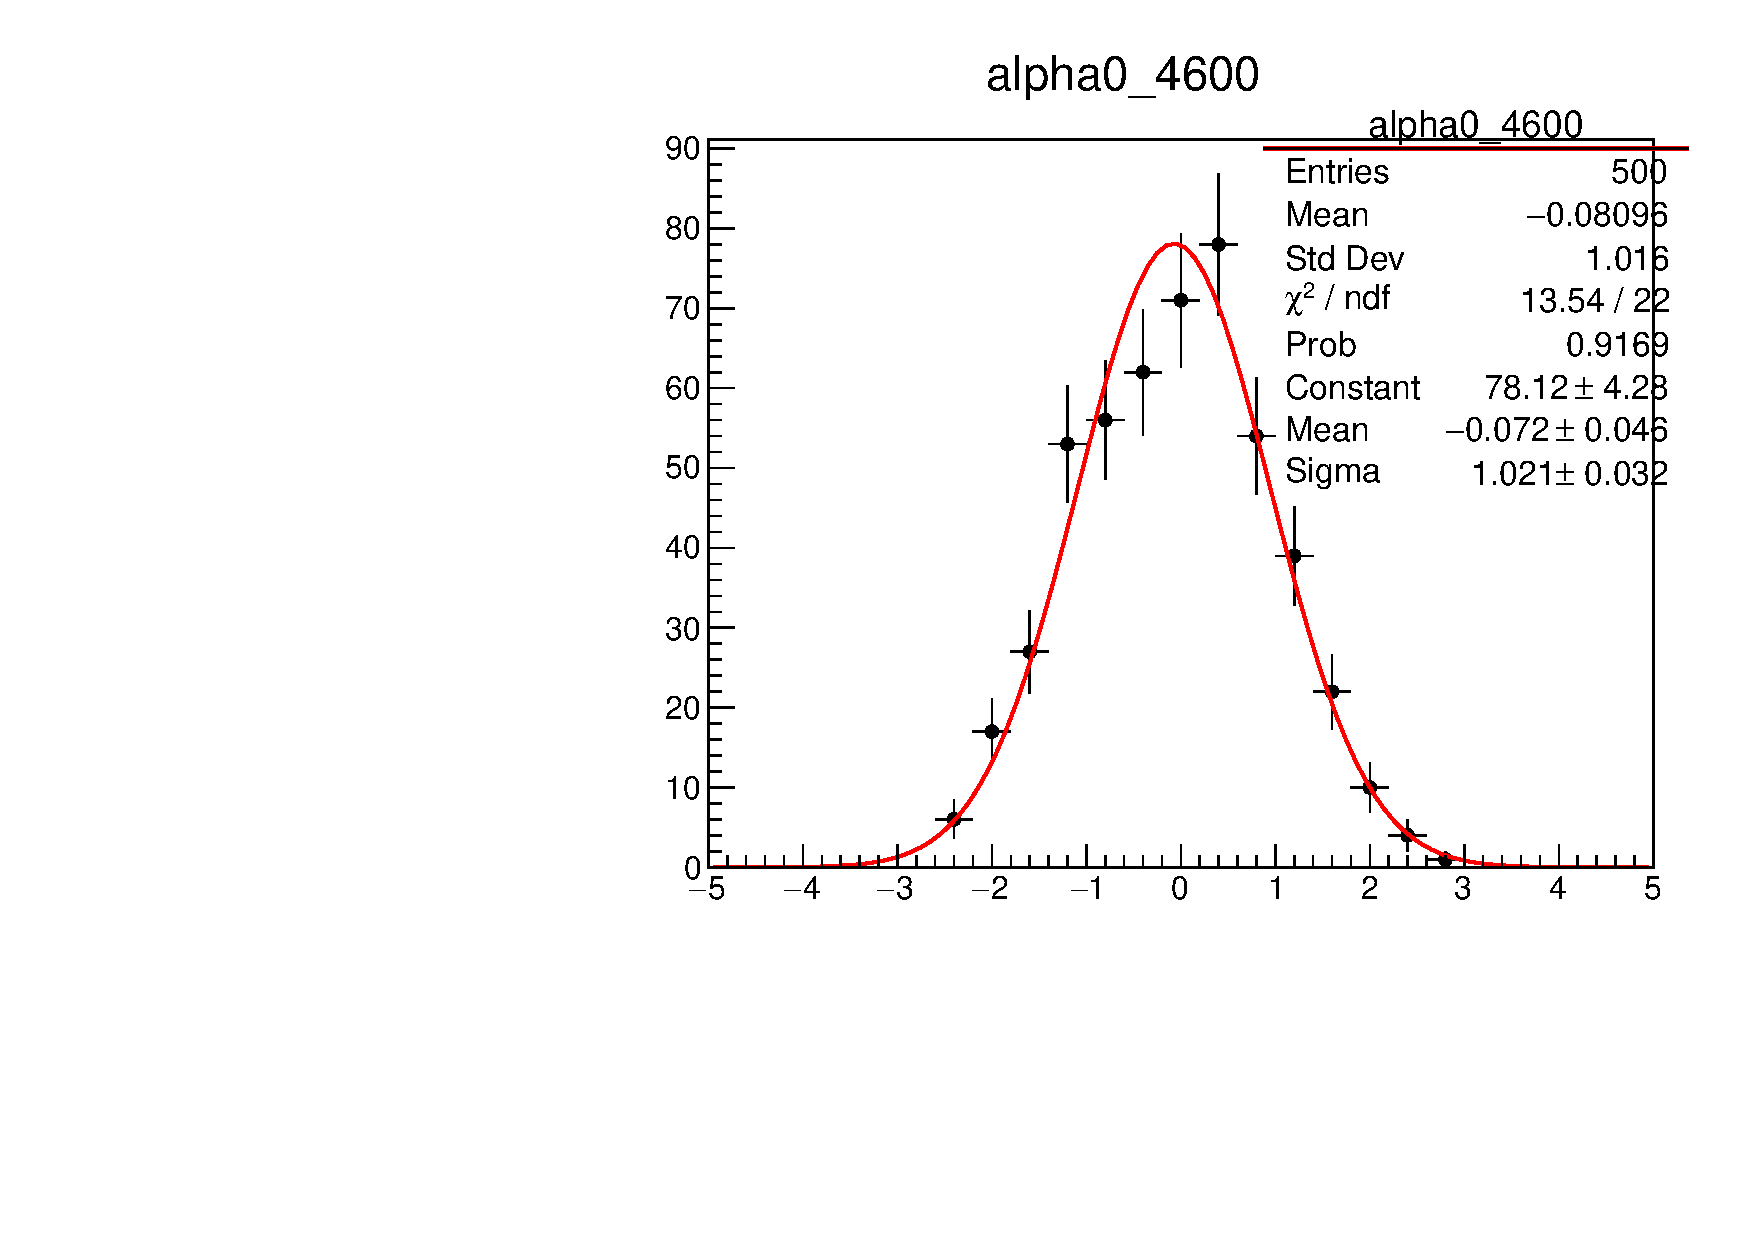
\includegraphics[width=0.24\textwidth]{figure/io_wo_bkg/polarization/pull_polarization_alpha0_4600.pdf}
    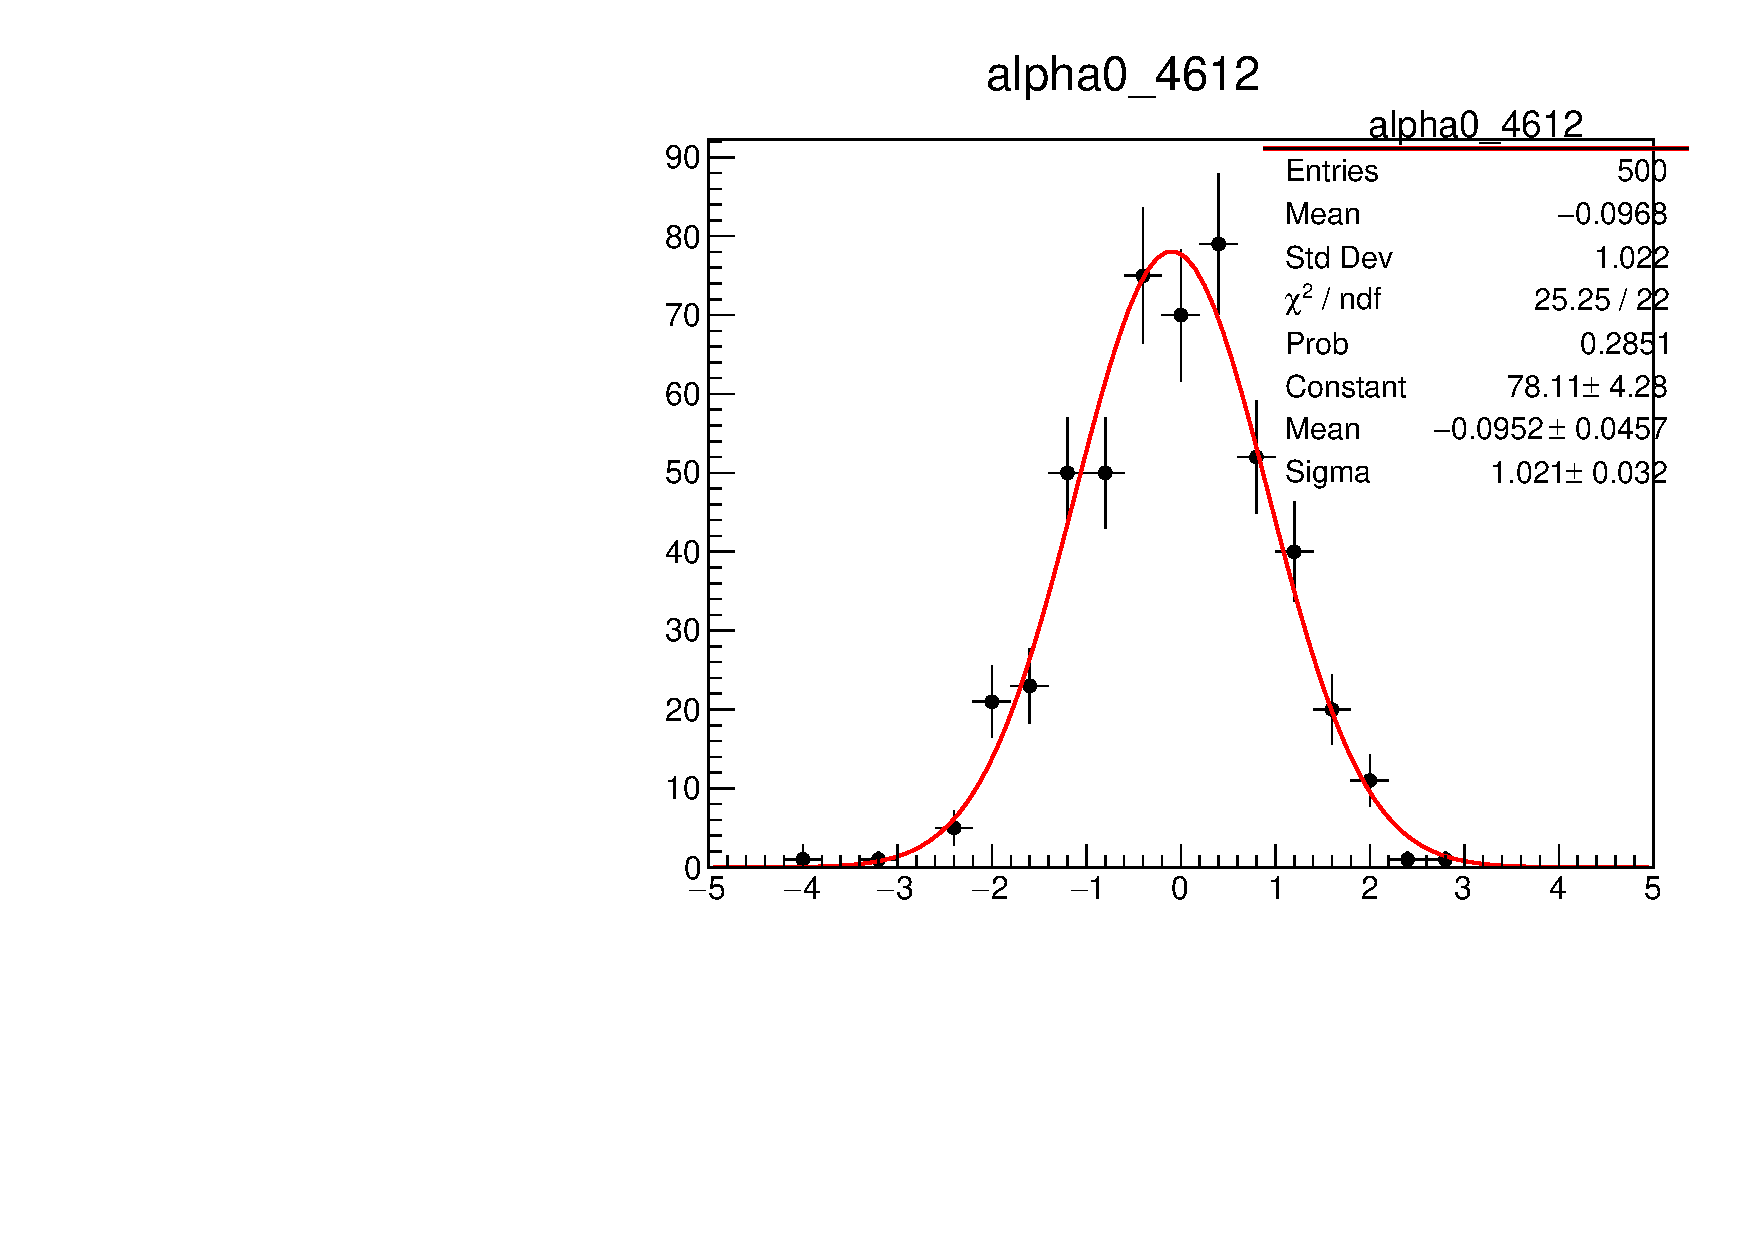
\includegraphics[width=0.24\textwidth]{figure/io_wo_bkg/polarization/pull_polarization_alpha0_4612.pdf}
    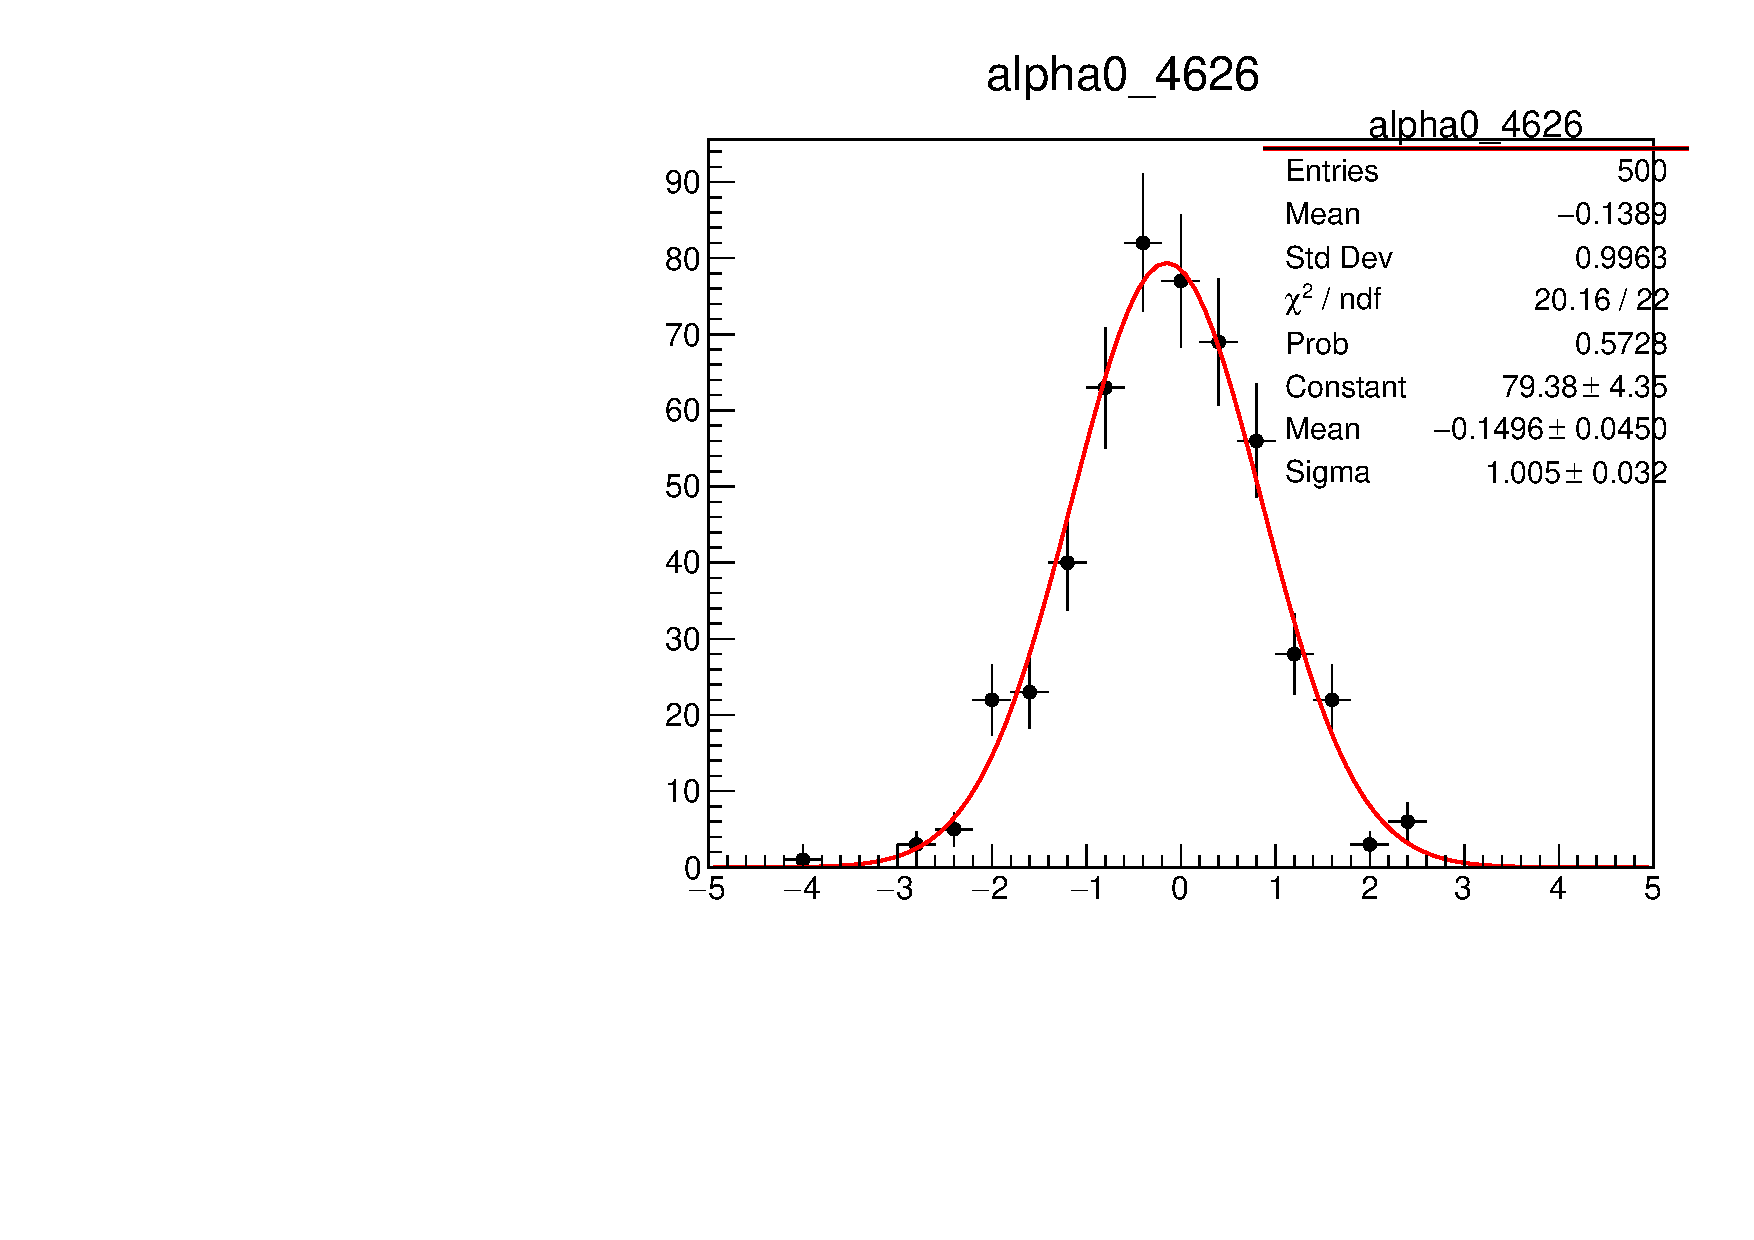
\includegraphics[width=0.24\textwidth]{figure/io_wo_bkg/polarization/pull_polarization_alpha0_4626.pdf}
    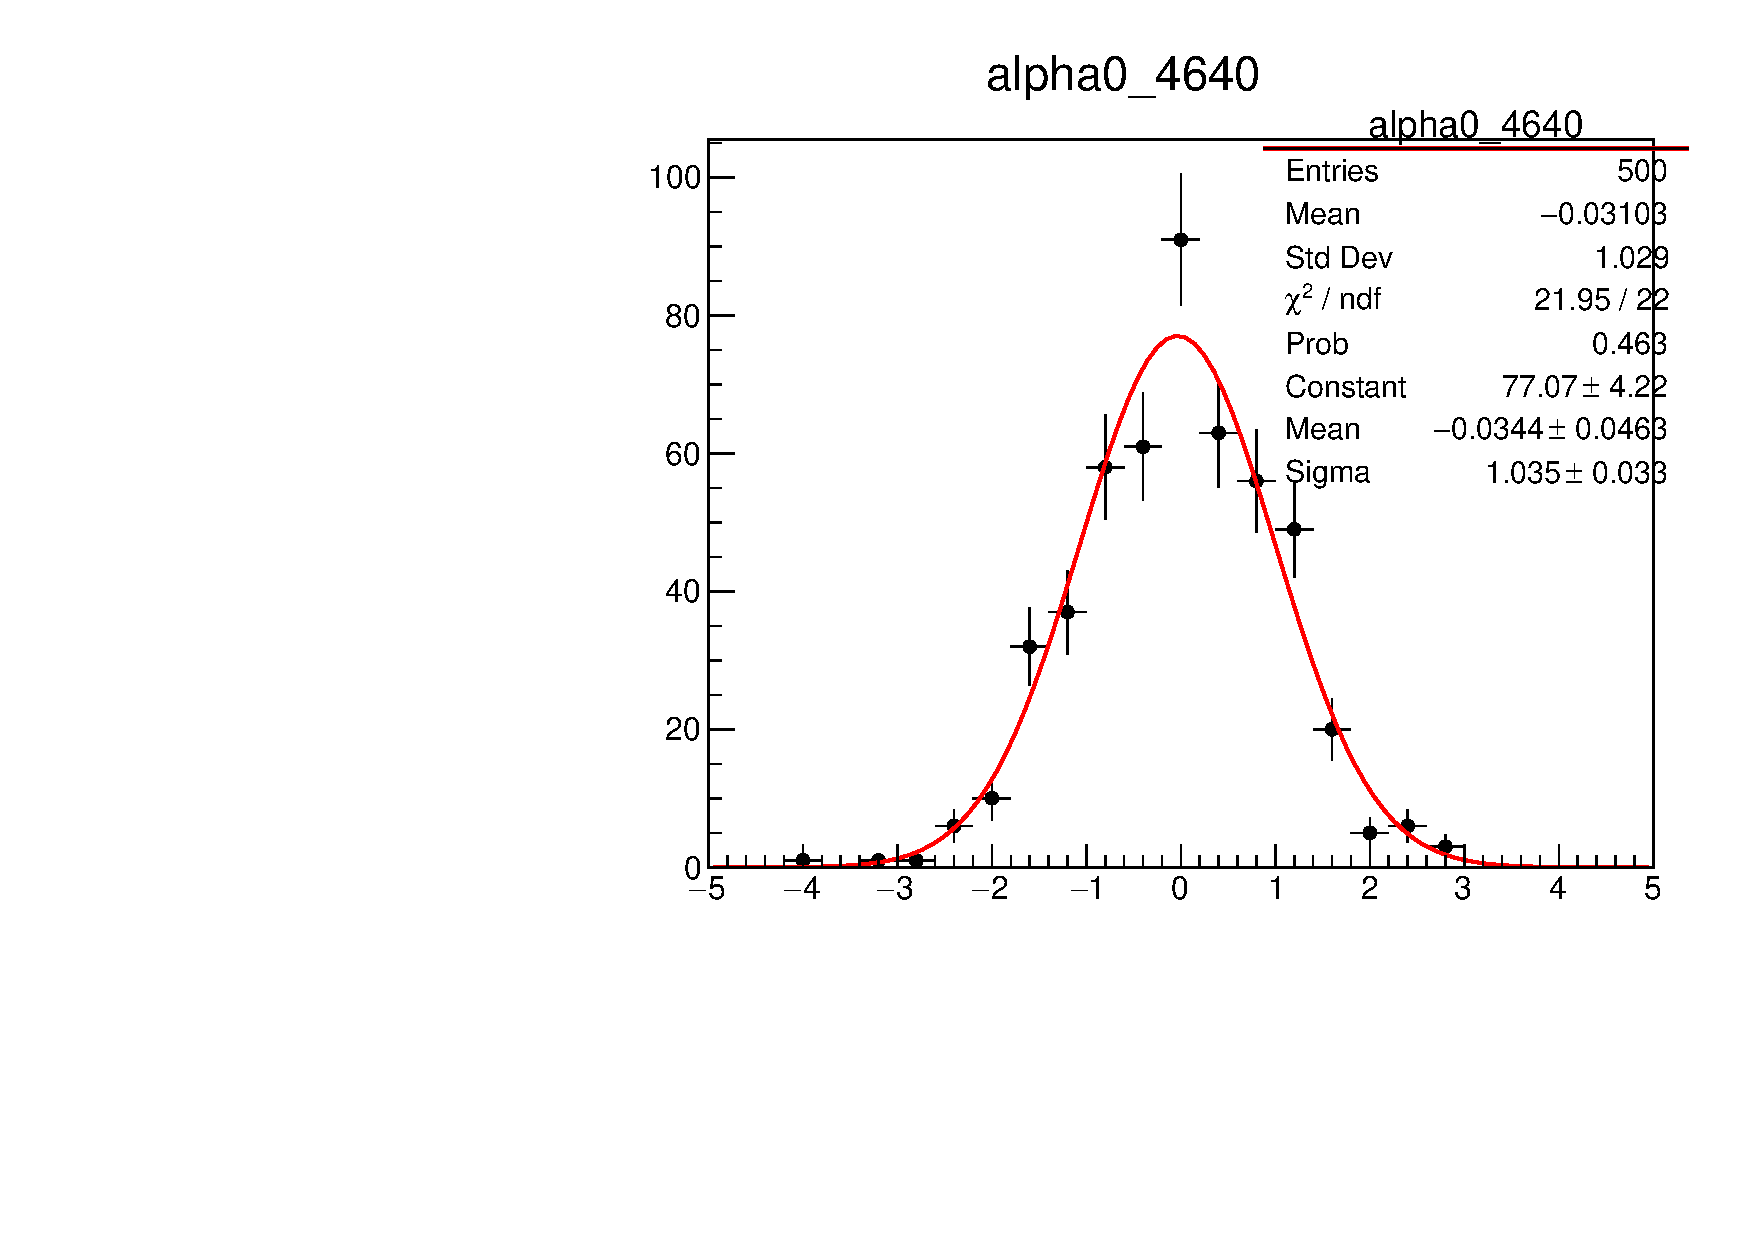
\includegraphics[width=0.24\textwidth]{figure/io_wo_bkg/polarization/pull_polarization_alpha0_4640.pdf}
    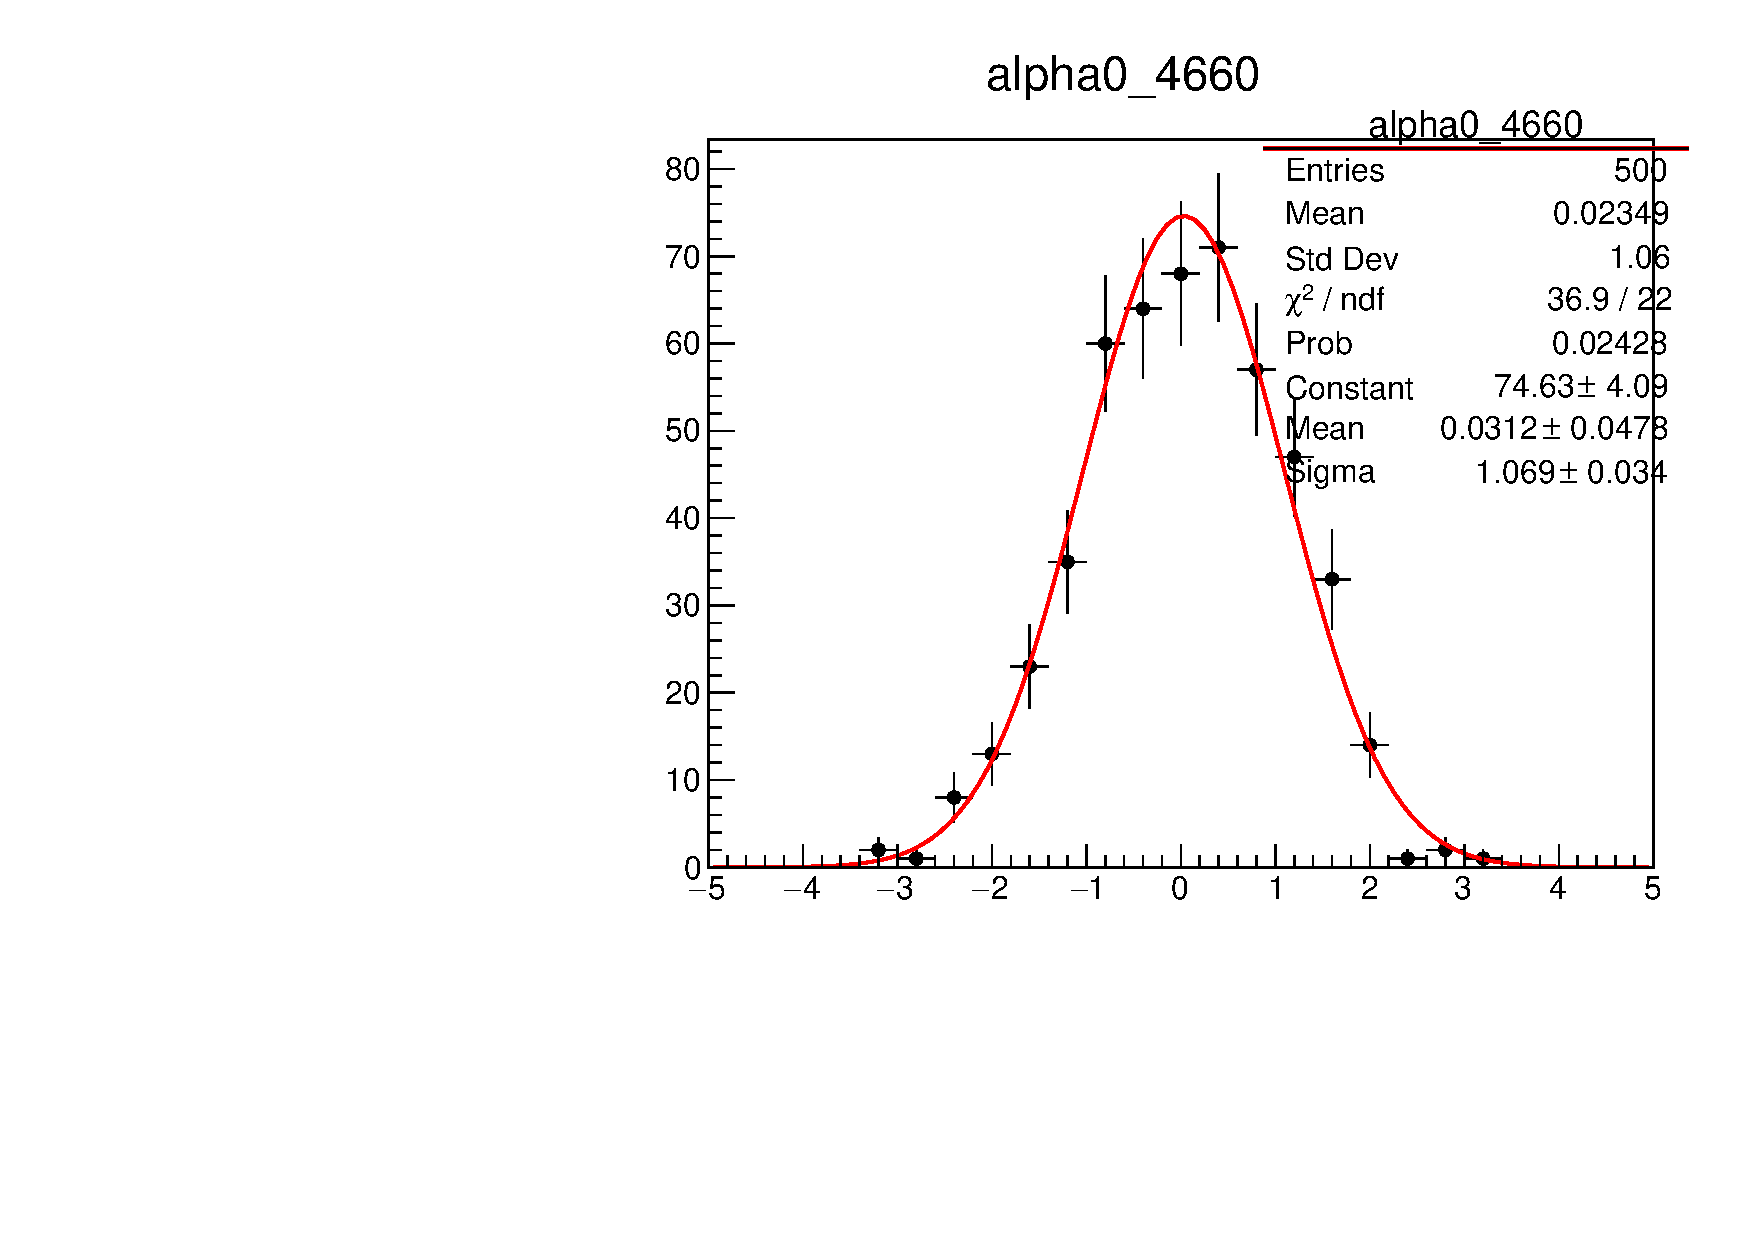
\includegraphics[width=0.24\textwidth]{figure/io_wo_bkg/polarization/pull_polarization_alpha0_4660.pdf}
    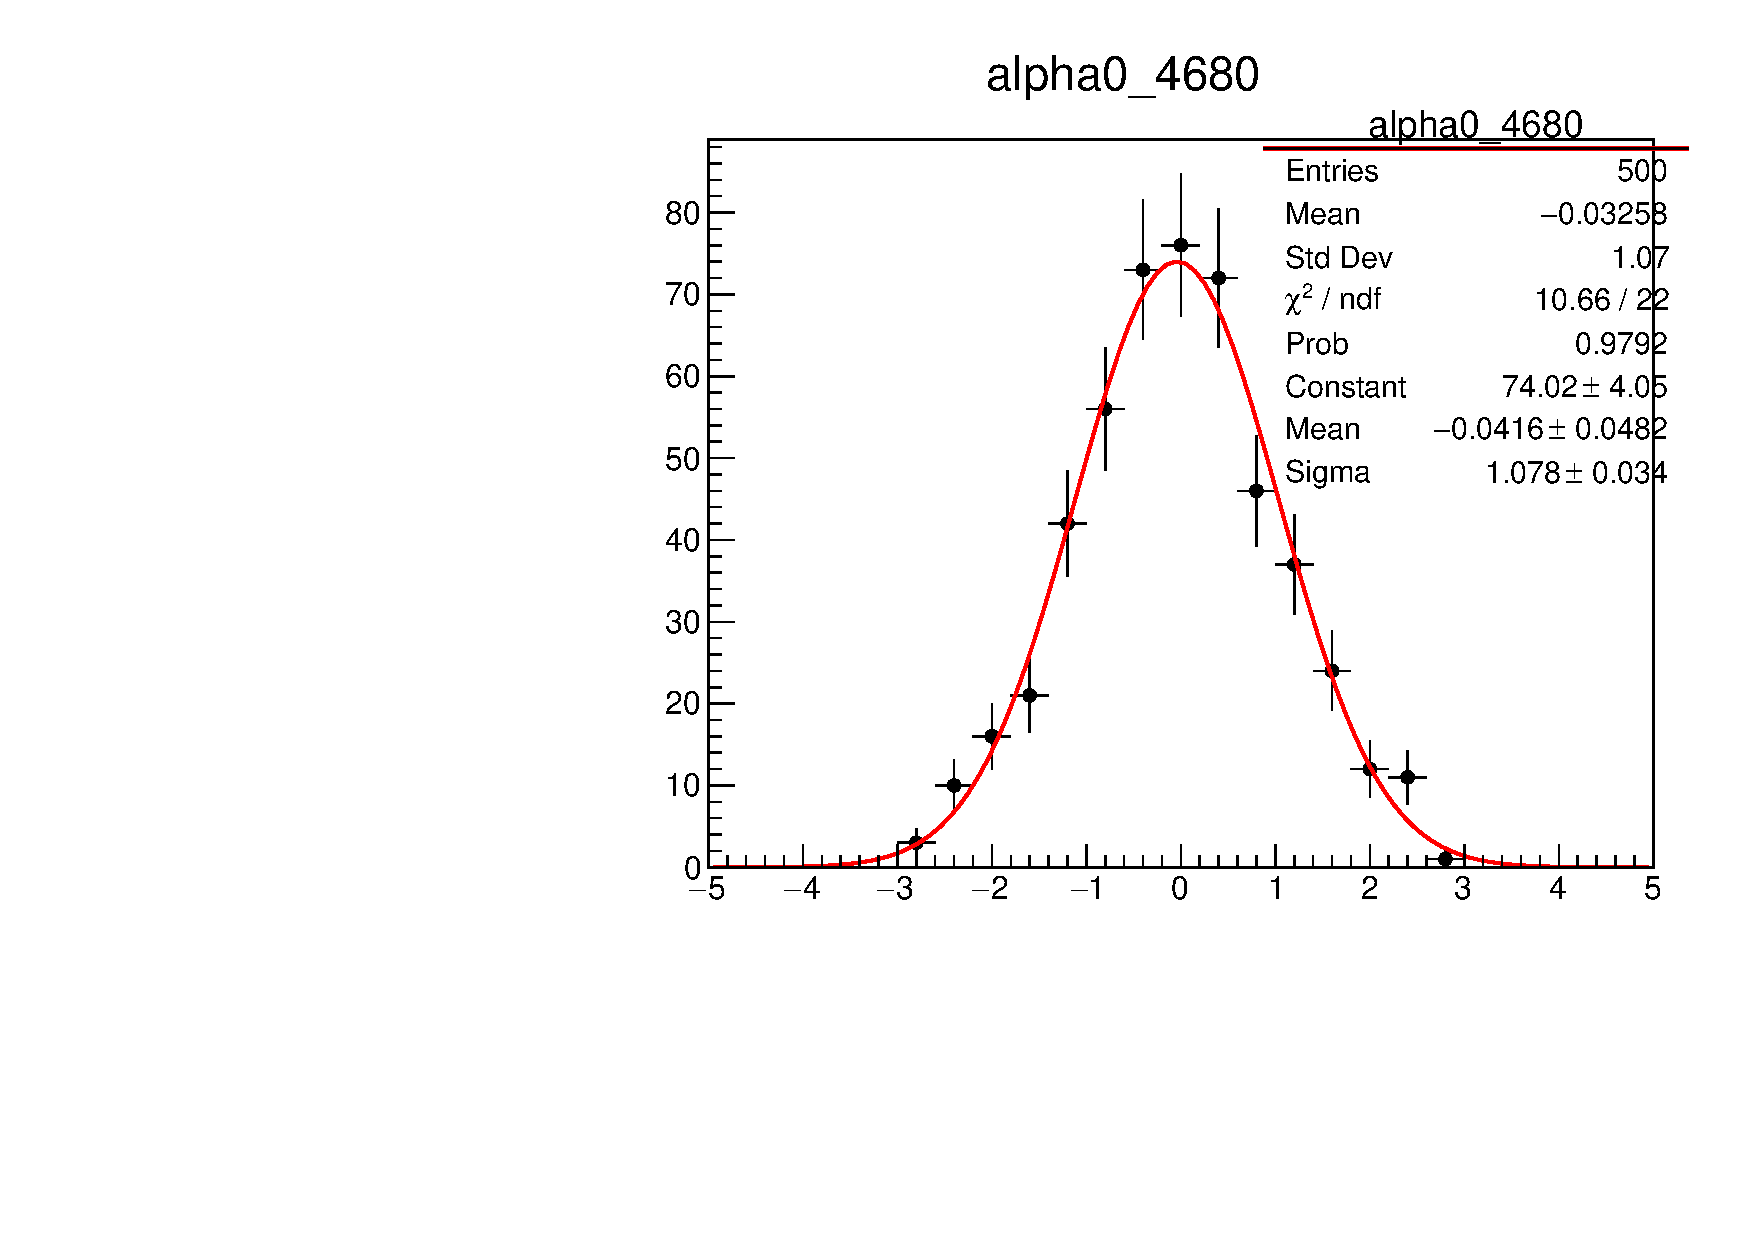
\includegraphics[width=0.24\textwidth]{figure/io_wo_bkg/polarization/pull_polarization_alpha0_4680.pdf}
    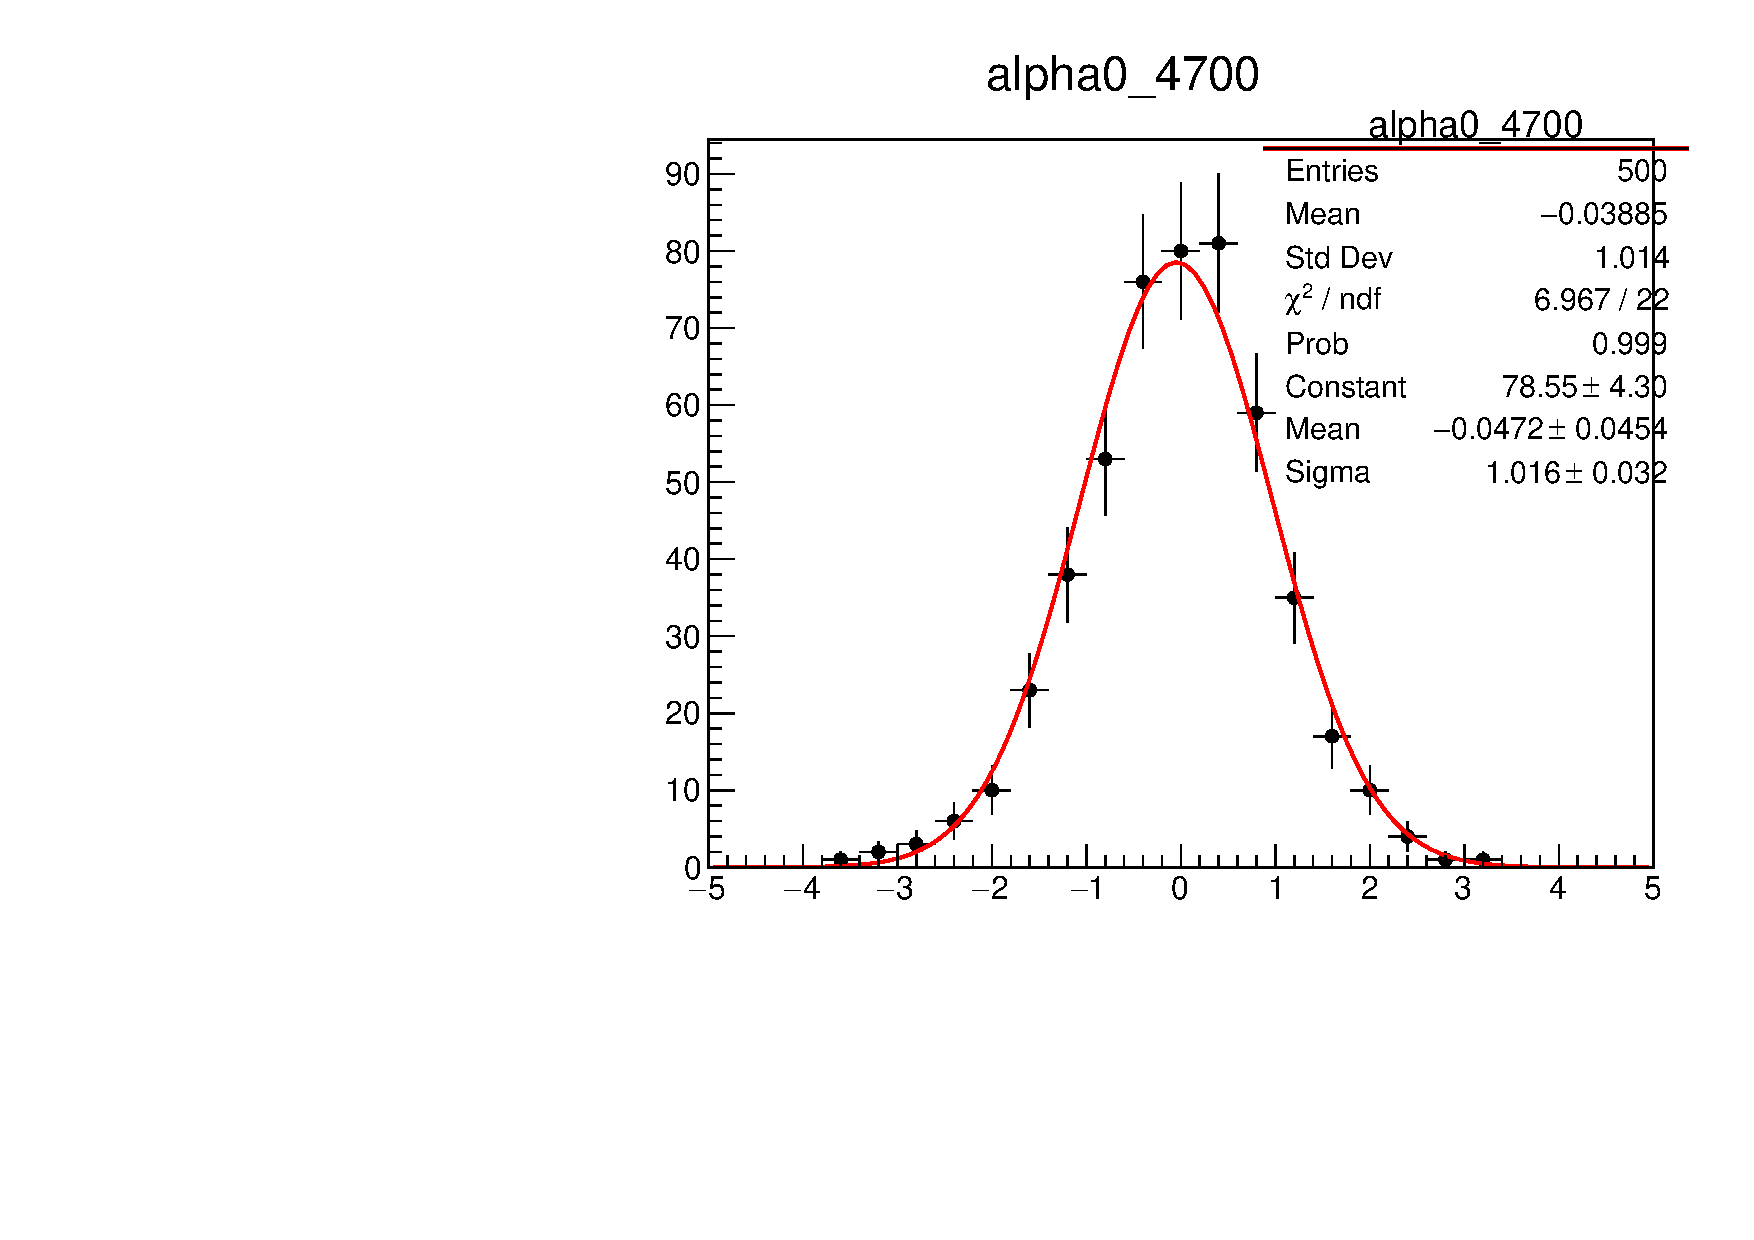
\includegraphics[width=0.24\textwidth]{figure/io_wo_bkg/polarization/pull_polarization_alpha0_4700.pdf}
    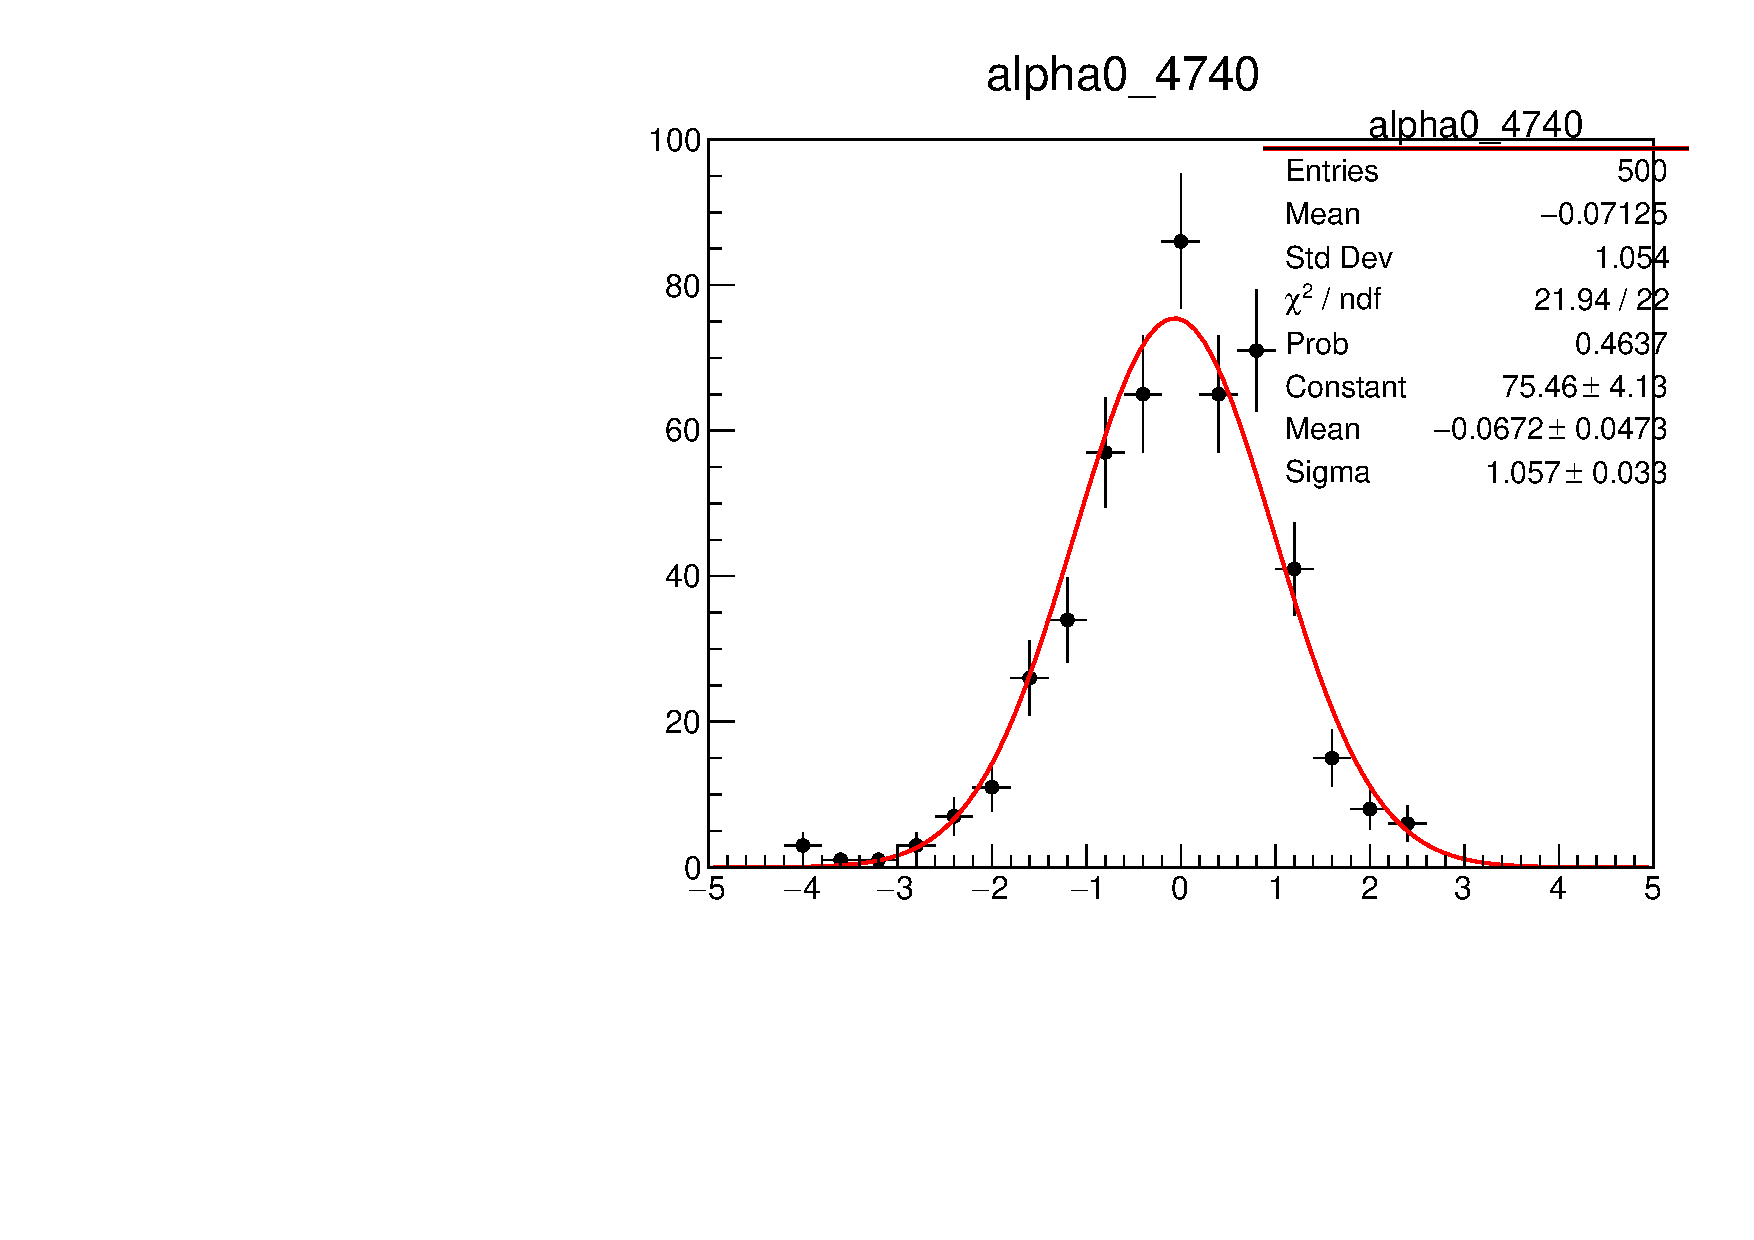
\includegraphics[width=0.24\textwidth]{figure/io_wo_bkg/polarization/pull_polarization_alpha0_4740.pdf}
    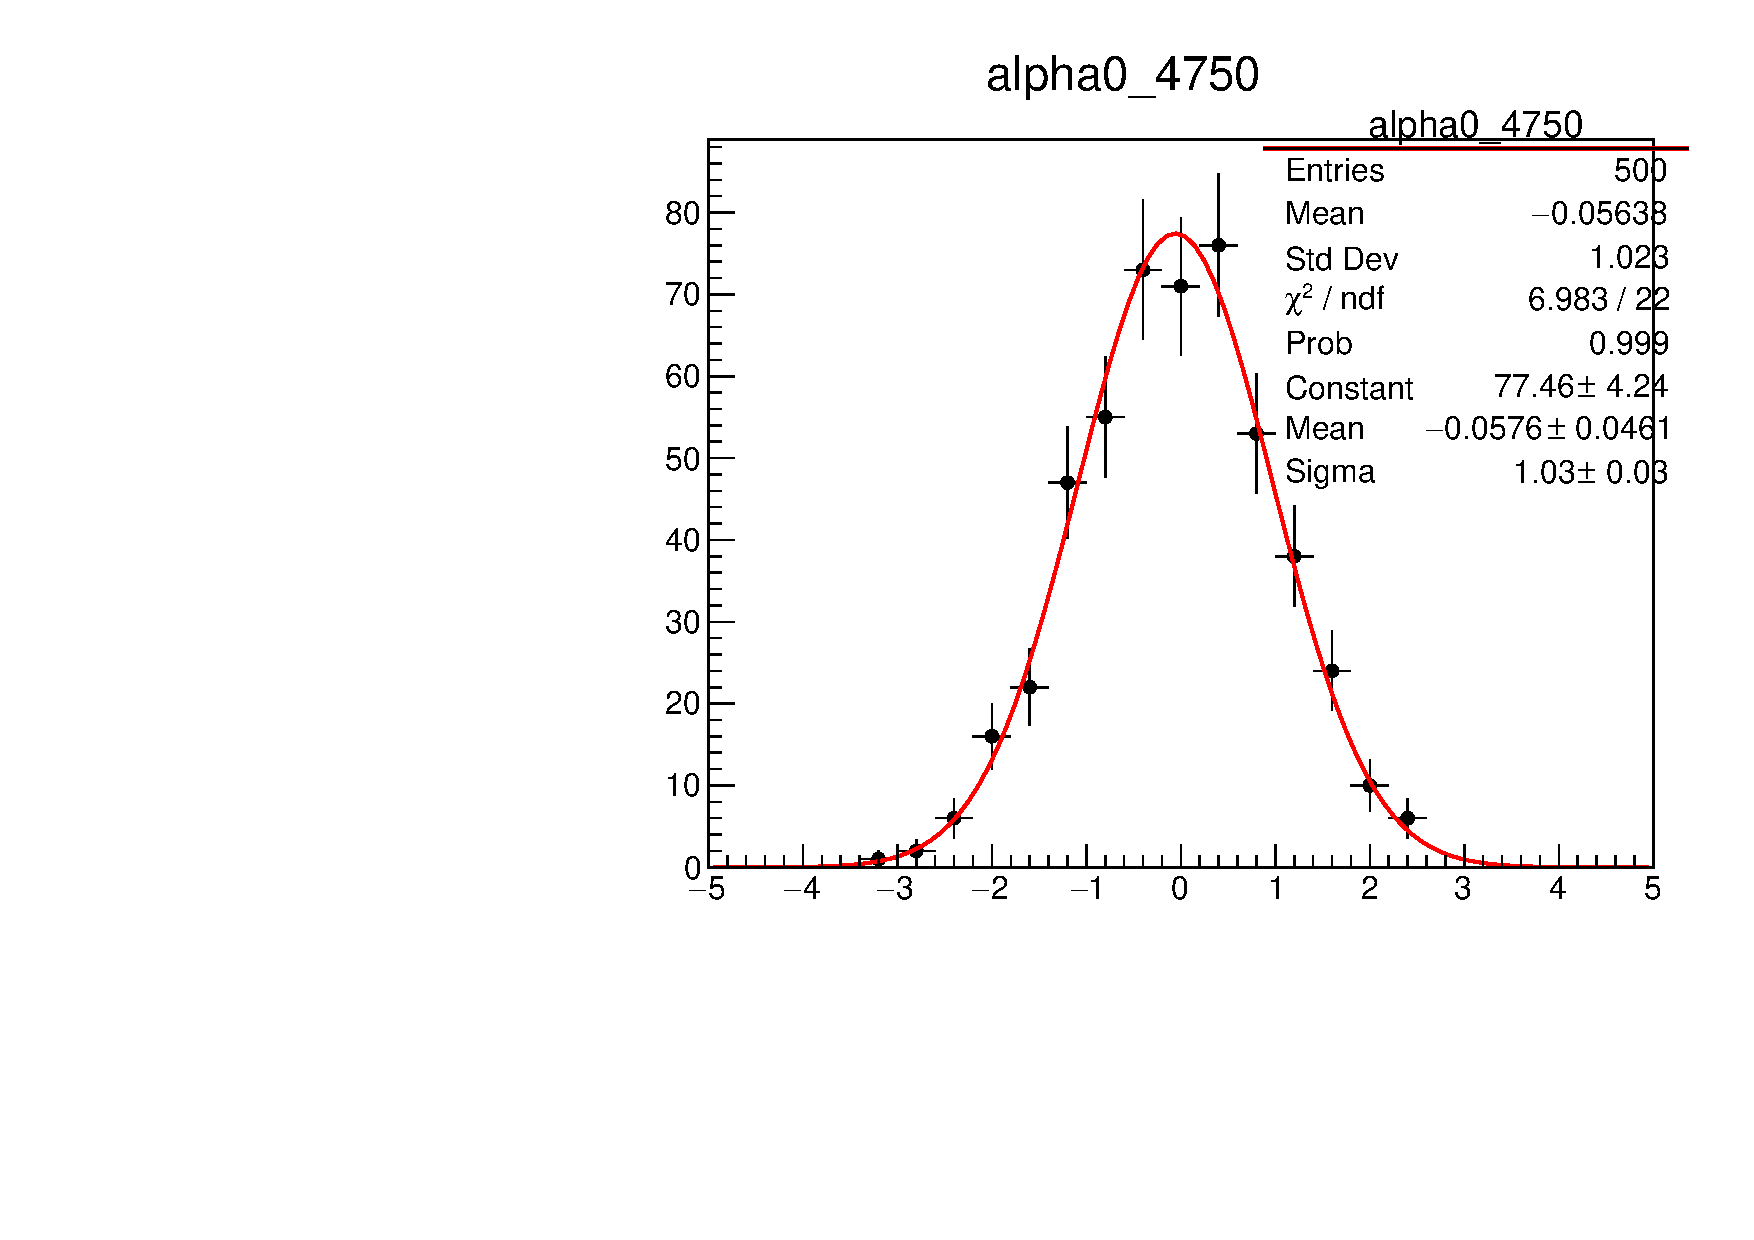
\includegraphics[width=0.24\textwidth]{figure/io_wo_bkg/polarization/pull_polarization_alpha0_4750.pdf}
    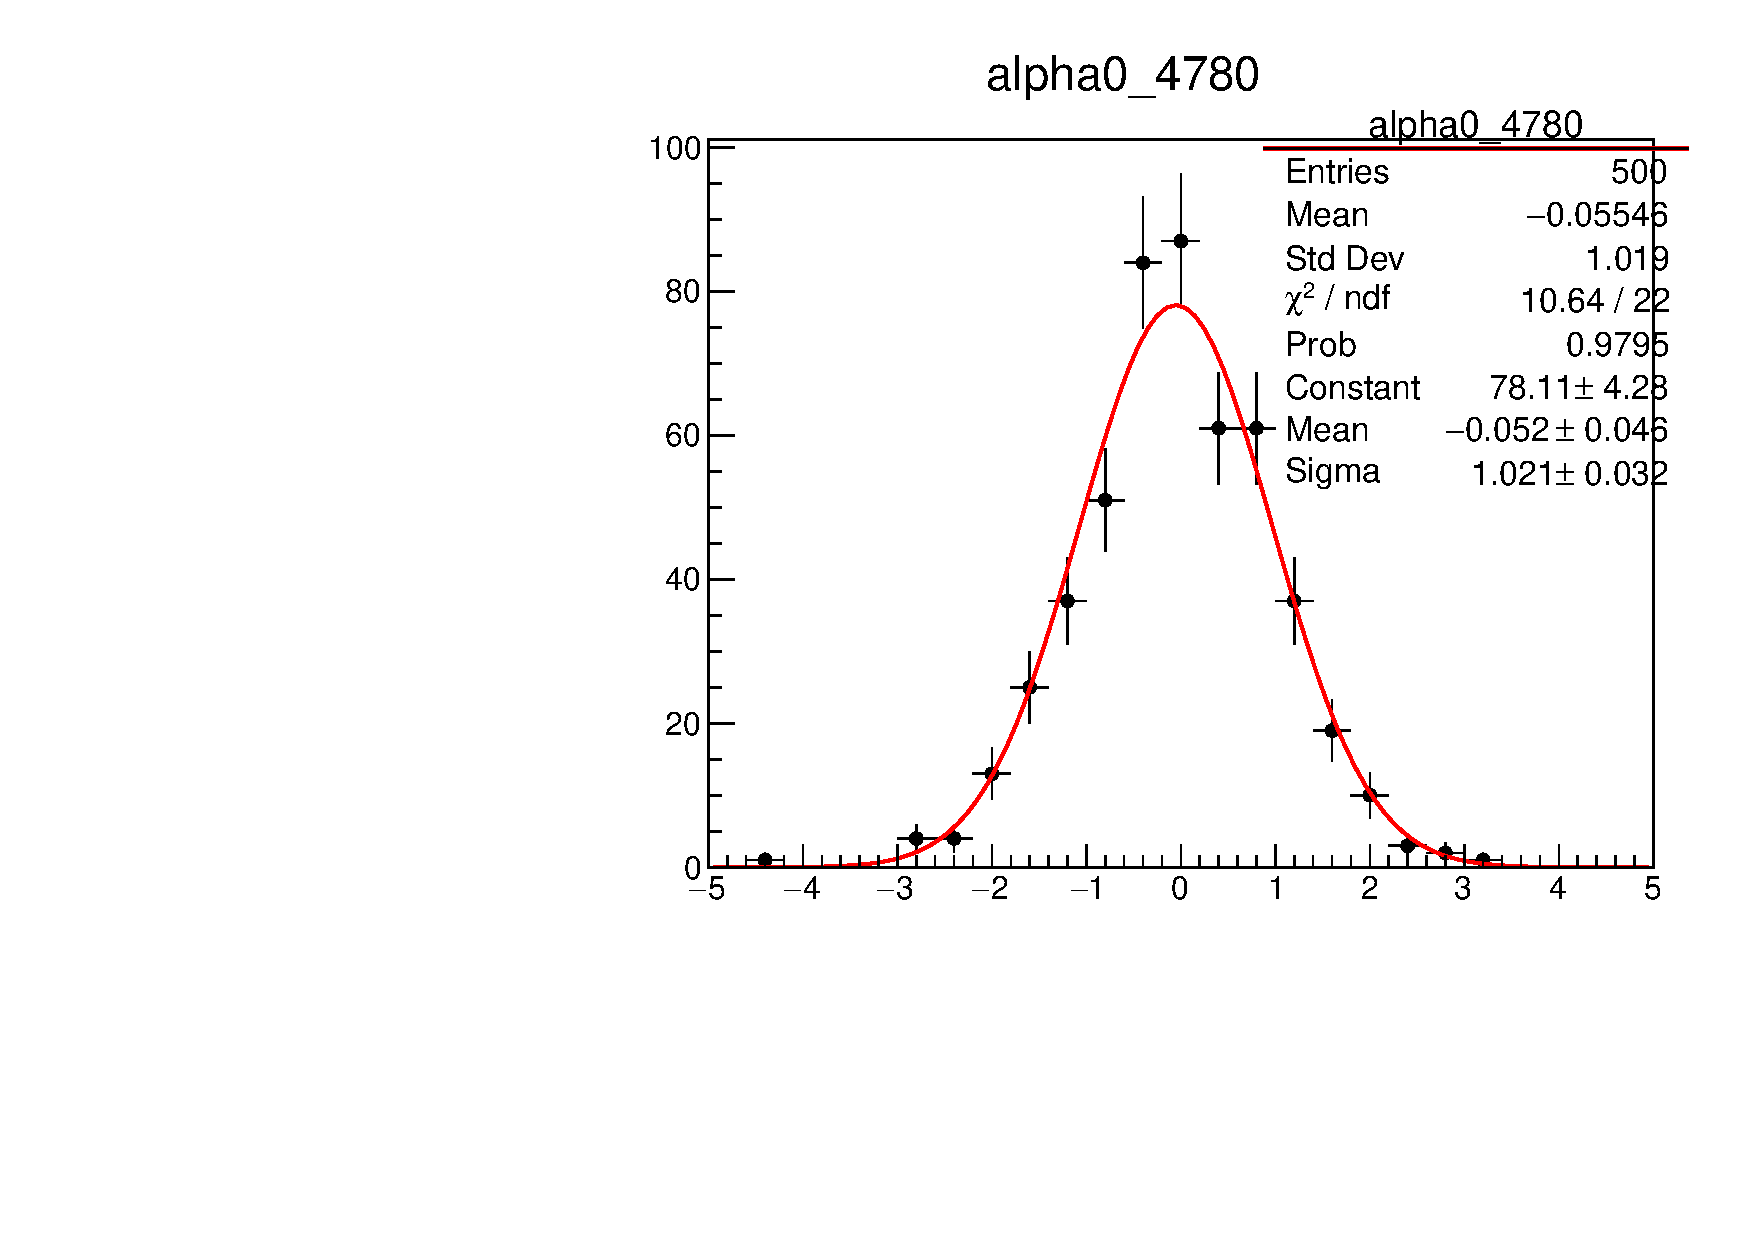
\includegraphics[width=0.24\textwidth]{figure/io_wo_bkg/polarization/pull_polarization_alpha0_4780.pdf}
    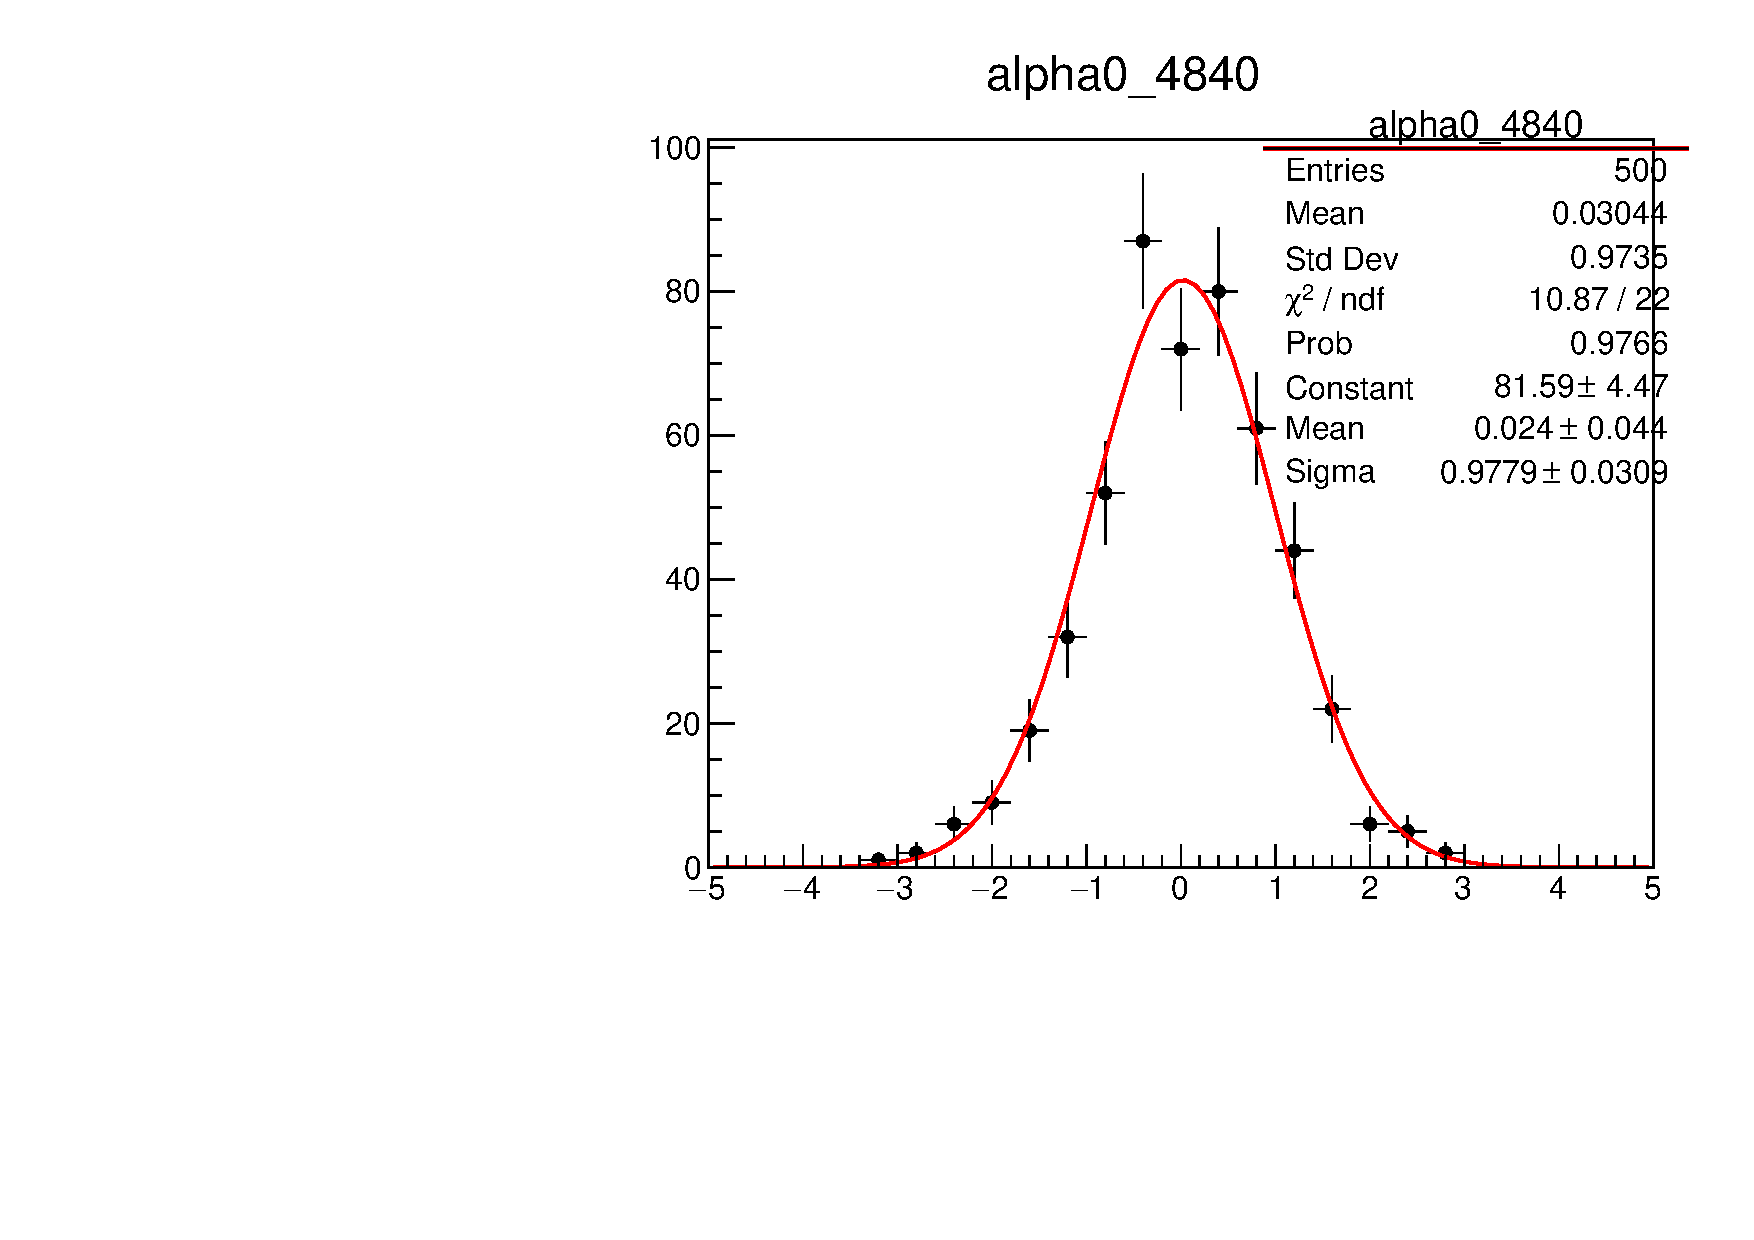
\includegraphics[width=0.24\textwidth]{figure/io_wo_bkg/polarization/pull_polarization_alpha0_4840.pdf}
    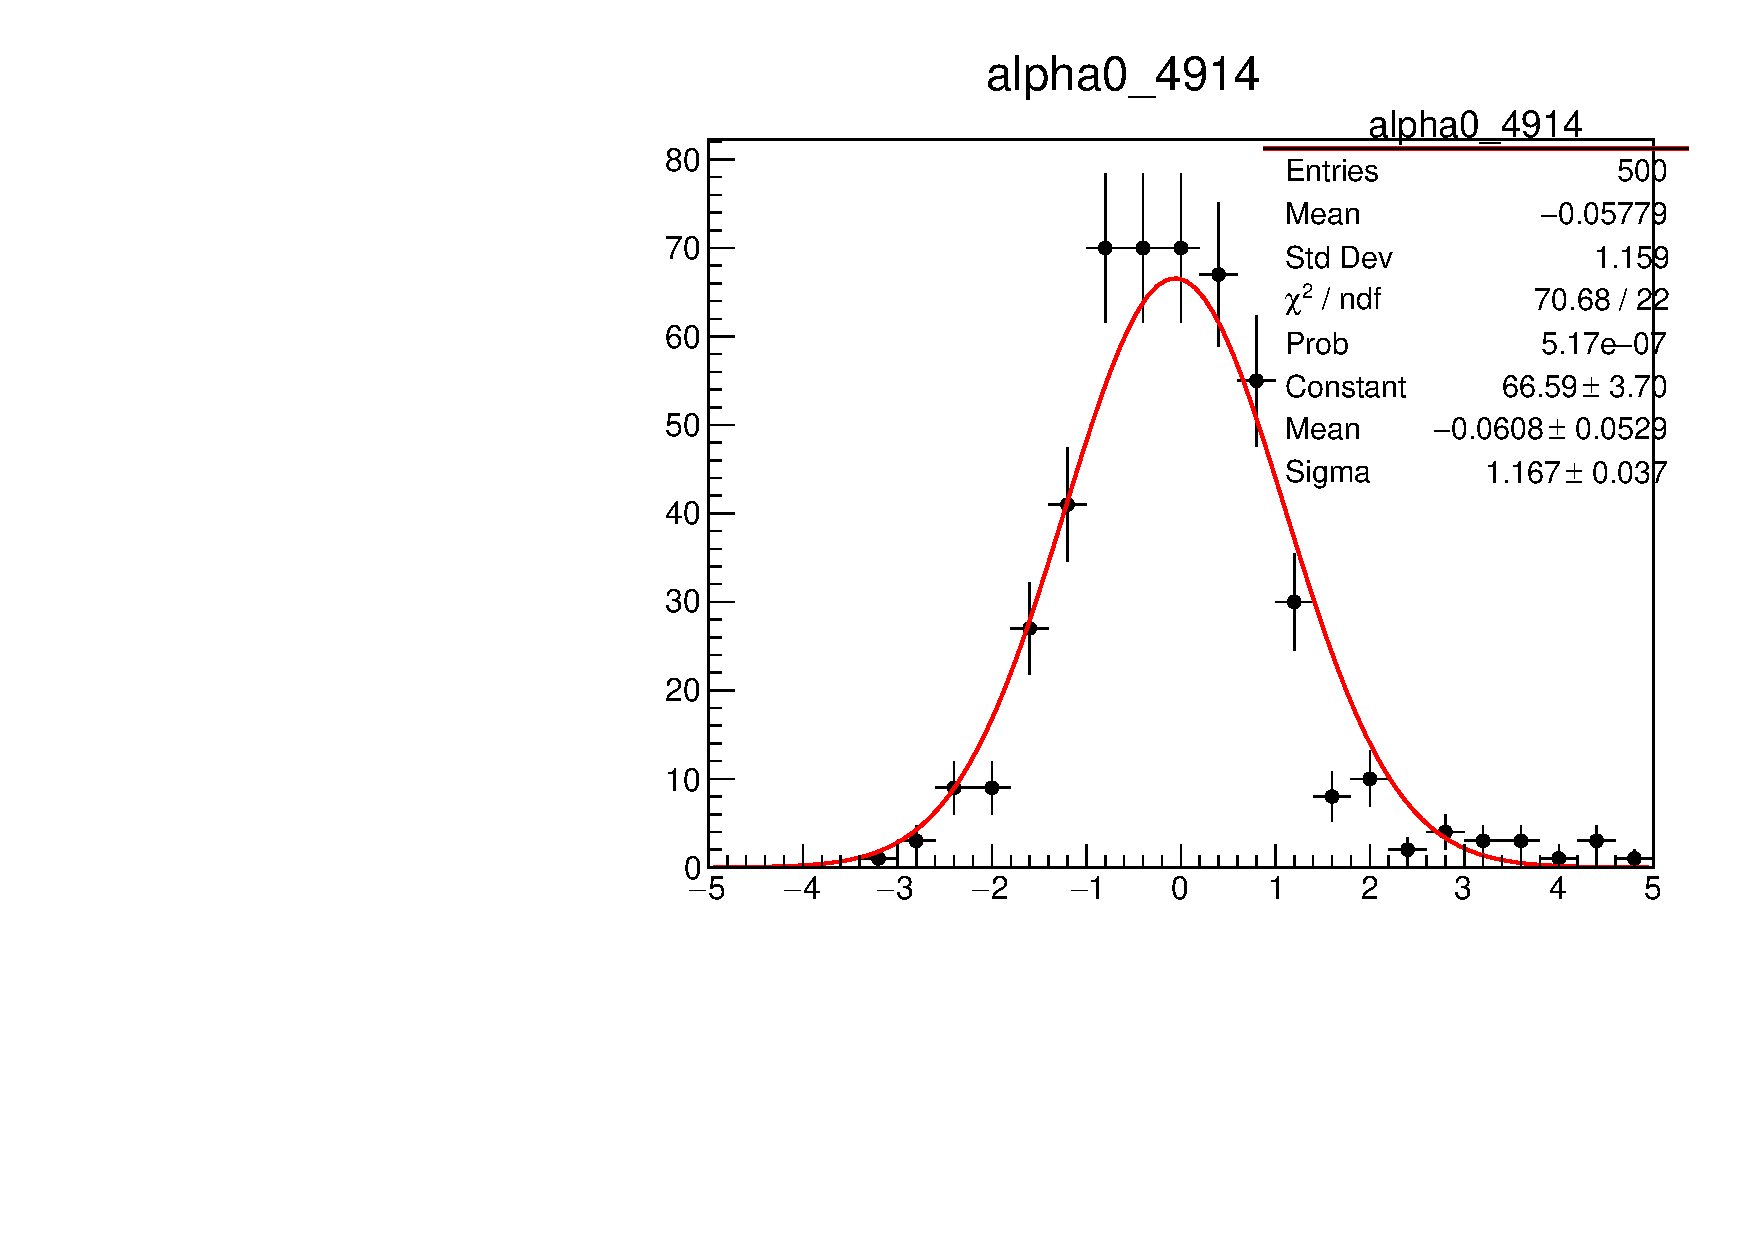
\includegraphics[width=0.24\textwidth]{figure/io_wo_bkg/polarization/pull_polarization_alpha0_4914.pdf}
    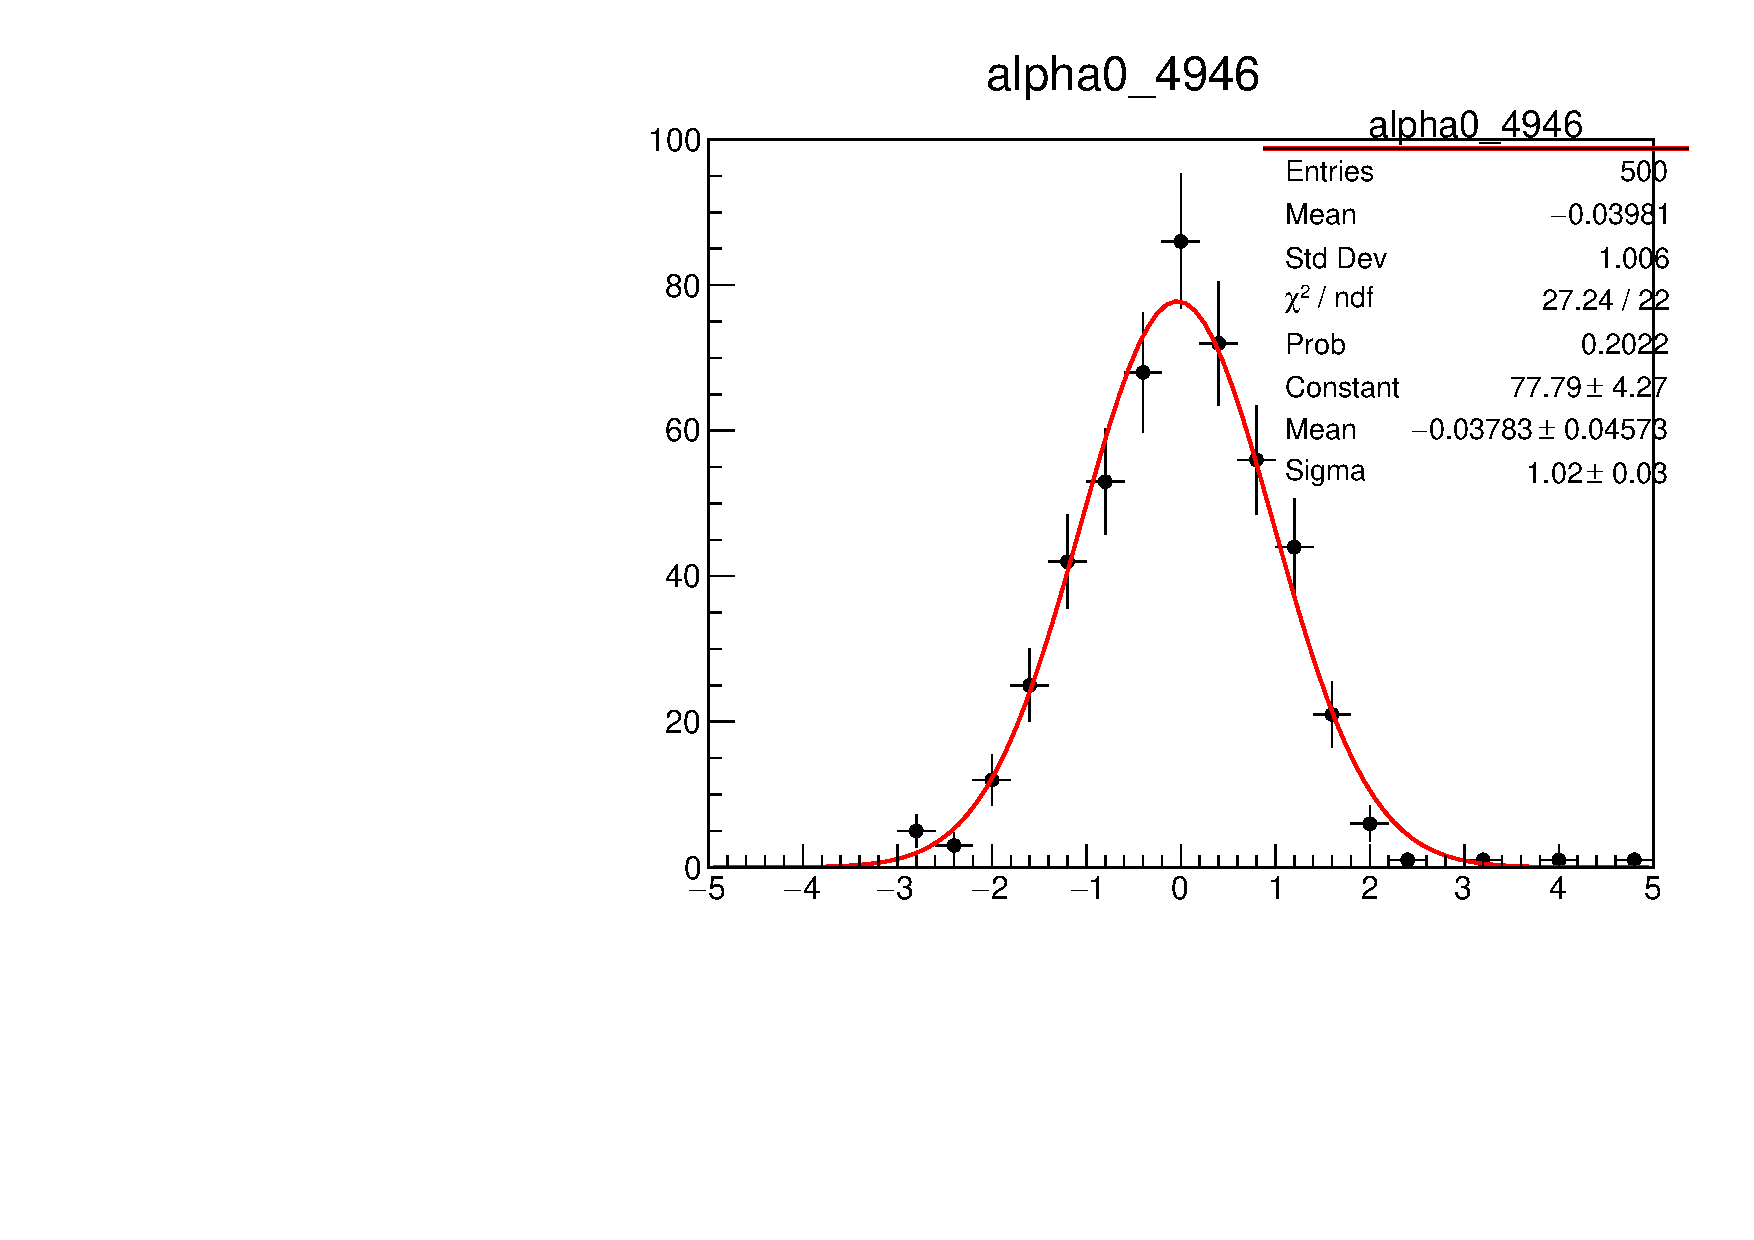
\includegraphics[width=0.24\textwidth]{figure/io_wo_bkg/polarization/pull_polarization_alpha0_4946.pdf}
    \caption{Pull distributions of $\alpha_0$ for each energy point.}
\label{fig:io_wo_bkg_pull_alpha0}
\end{figure}

\begin{figure}[h]\centering
    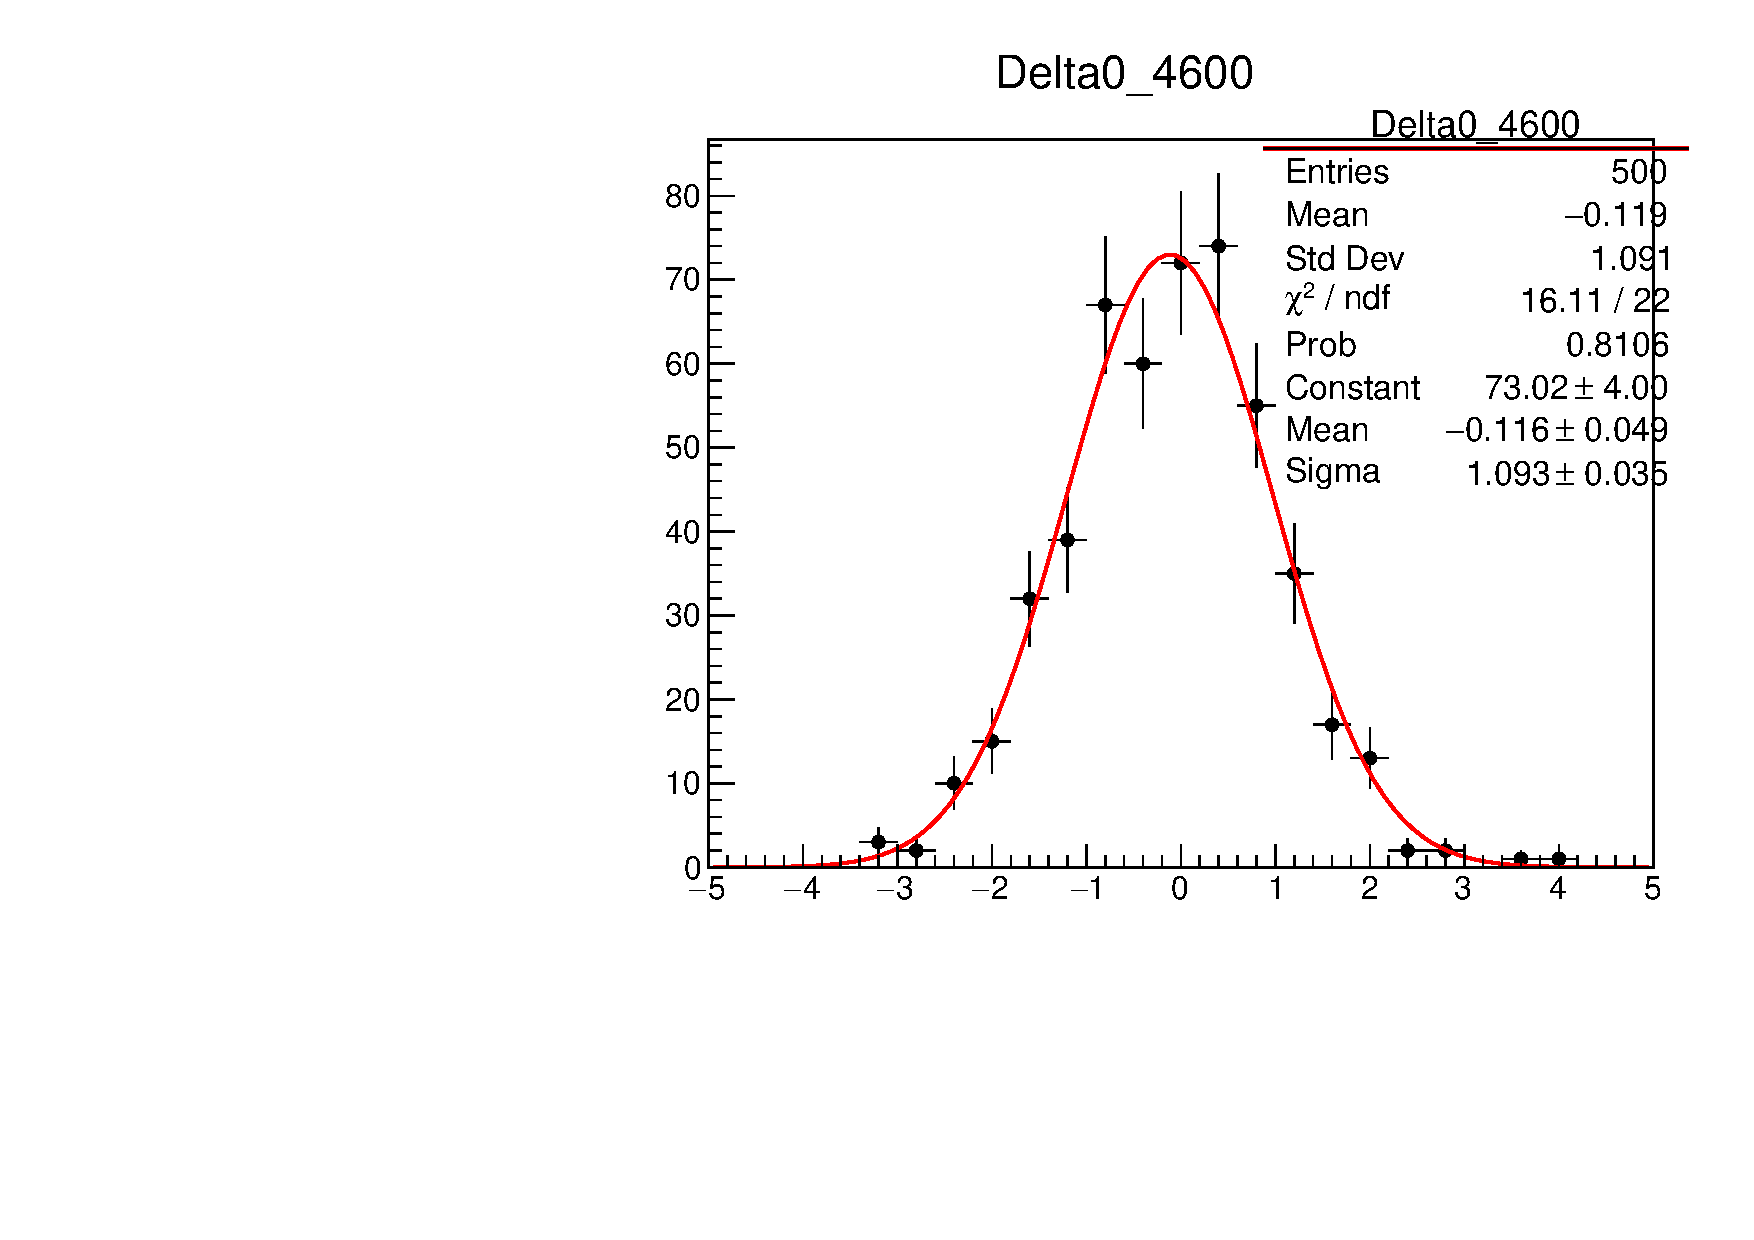
\includegraphics[width=0.24\textwidth]{figure/io_wo_bkg/polarization/pull_polarization_delta0_4600.pdf}
    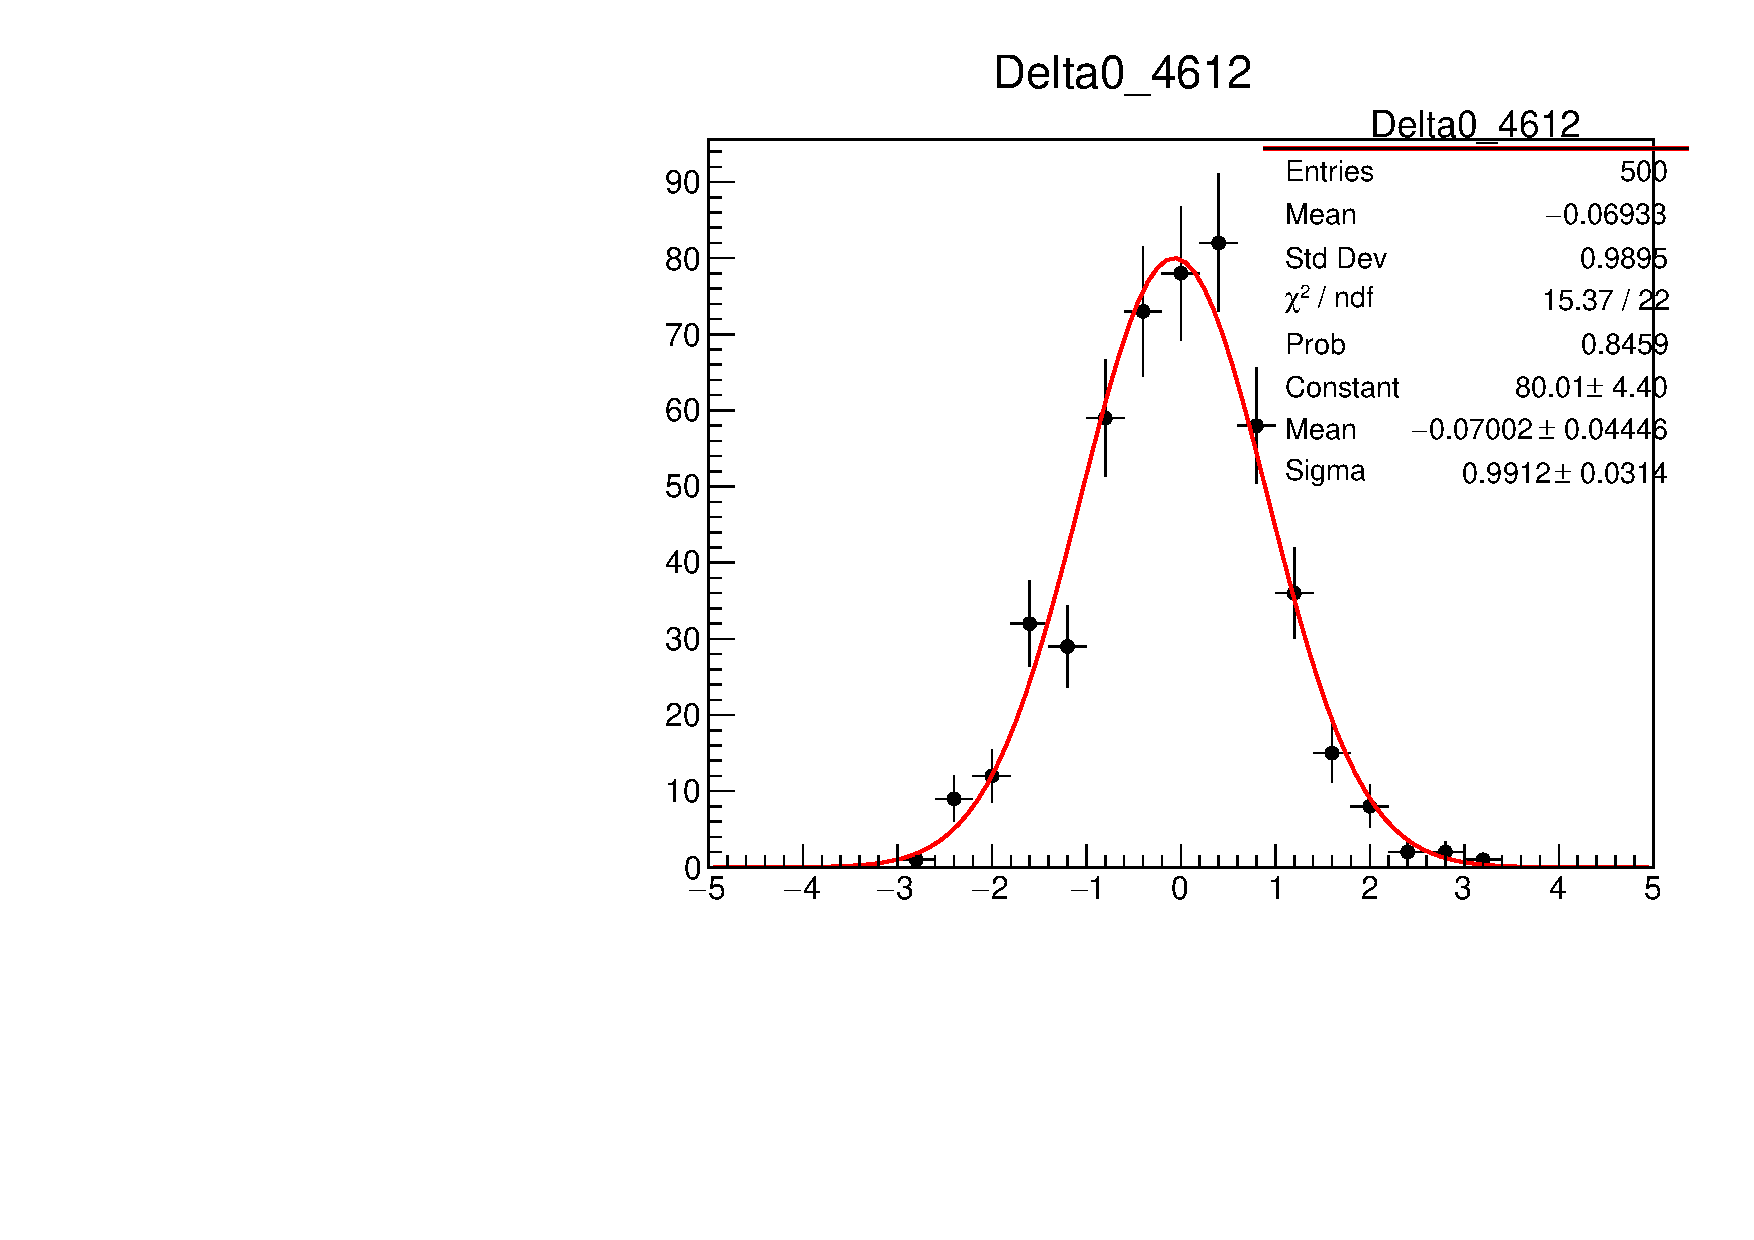
\includegraphics[width=0.24\textwidth]{figure/io_wo_bkg/polarization/pull_polarization_delta0_4612.pdf}
    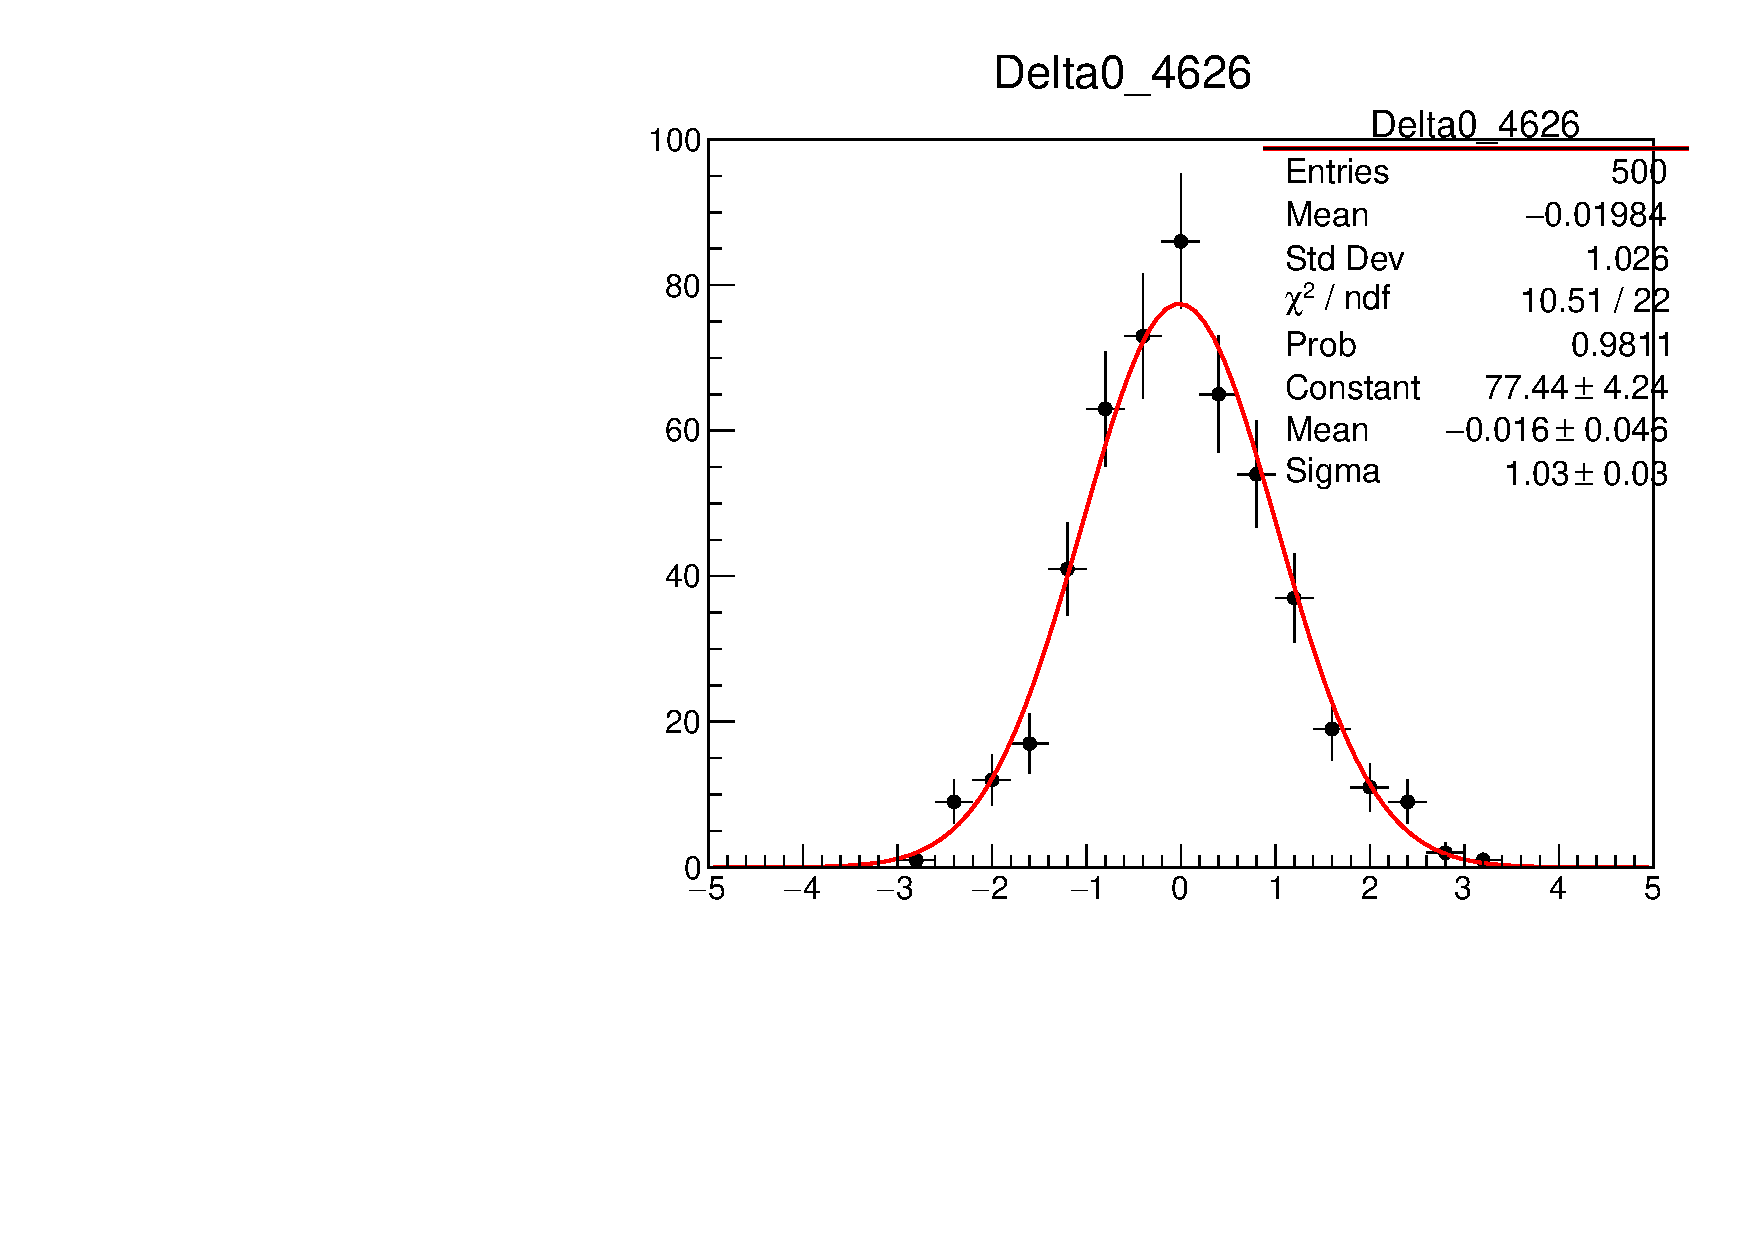
\includegraphics[width=0.24\textwidth]{figure/io_wo_bkg/polarization/pull_polarization_delta0_4626.pdf}
    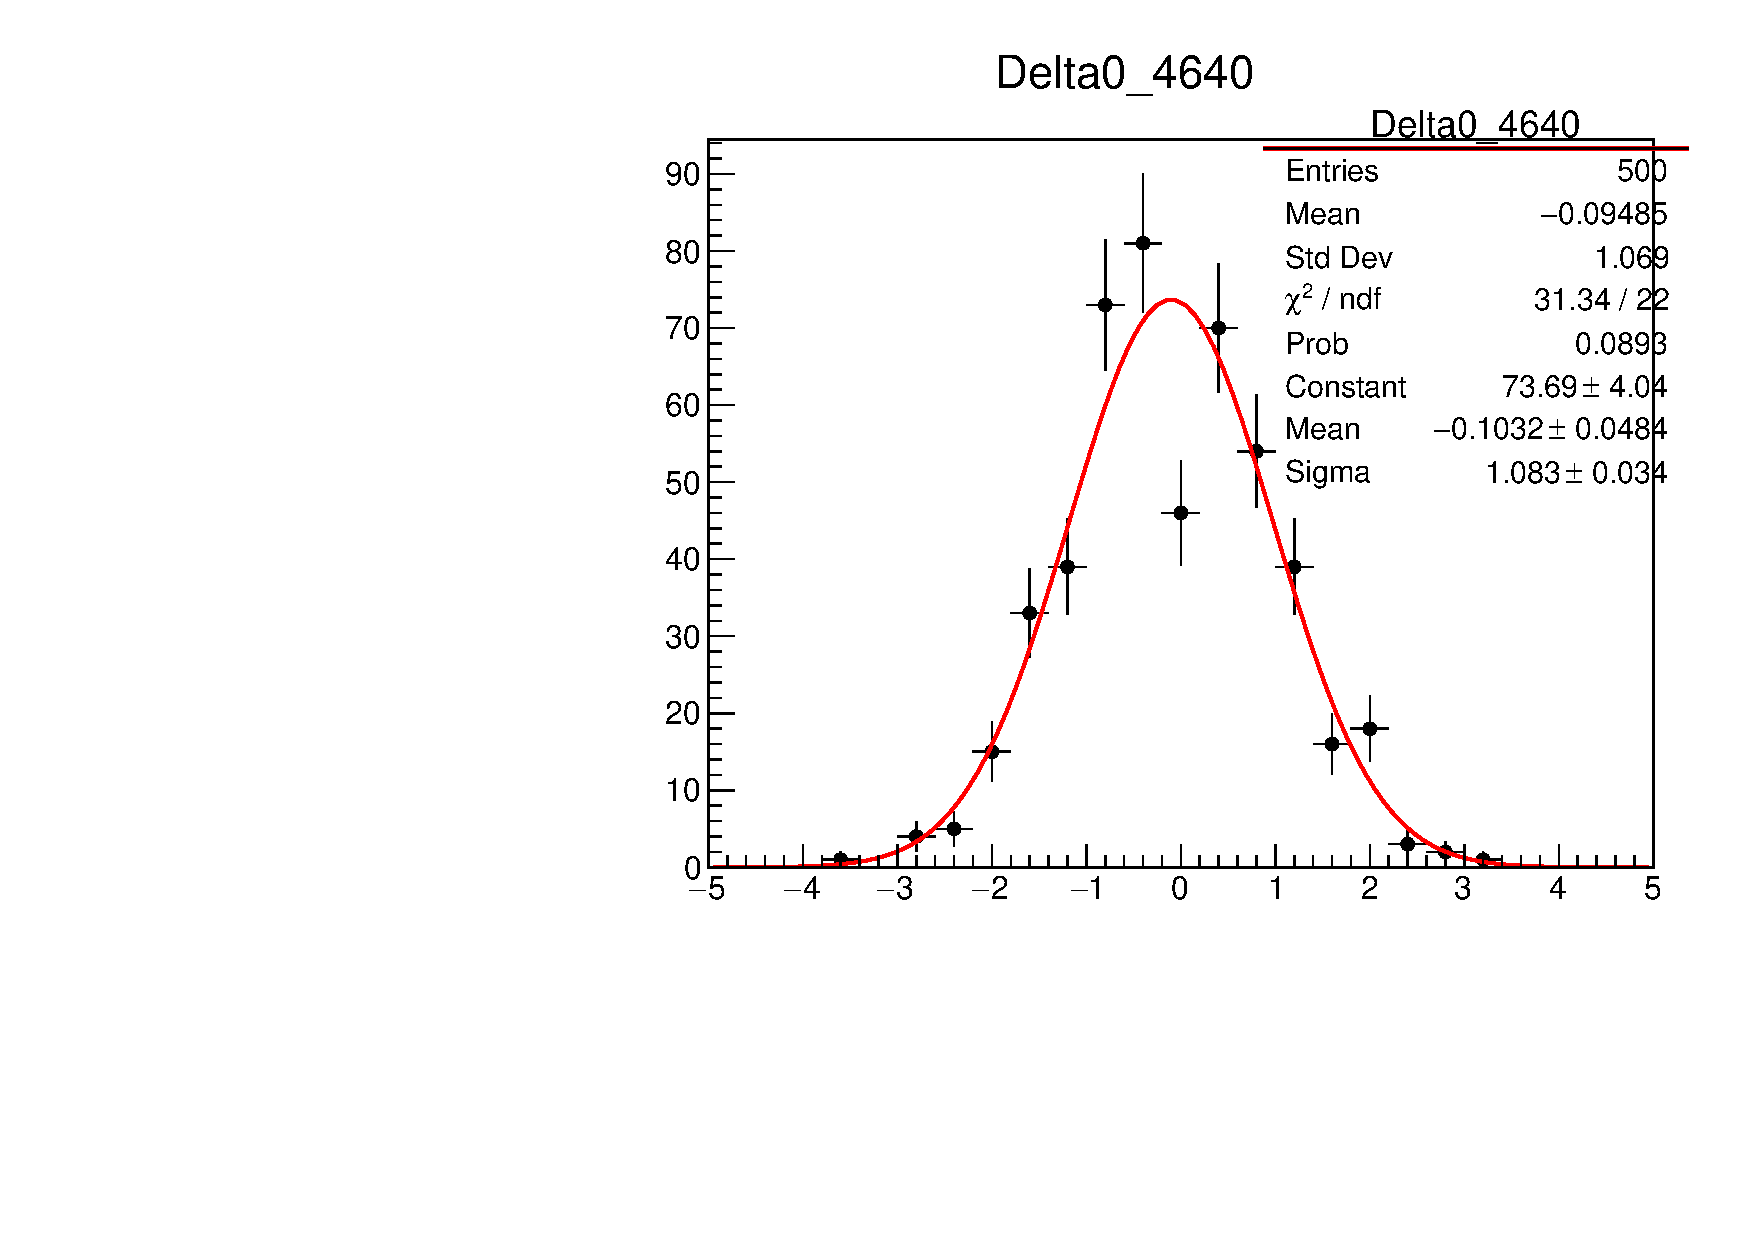
\includegraphics[width=0.24\textwidth]{figure/io_wo_bkg/polarization/pull_polarization_delta0_4640.pdf}
    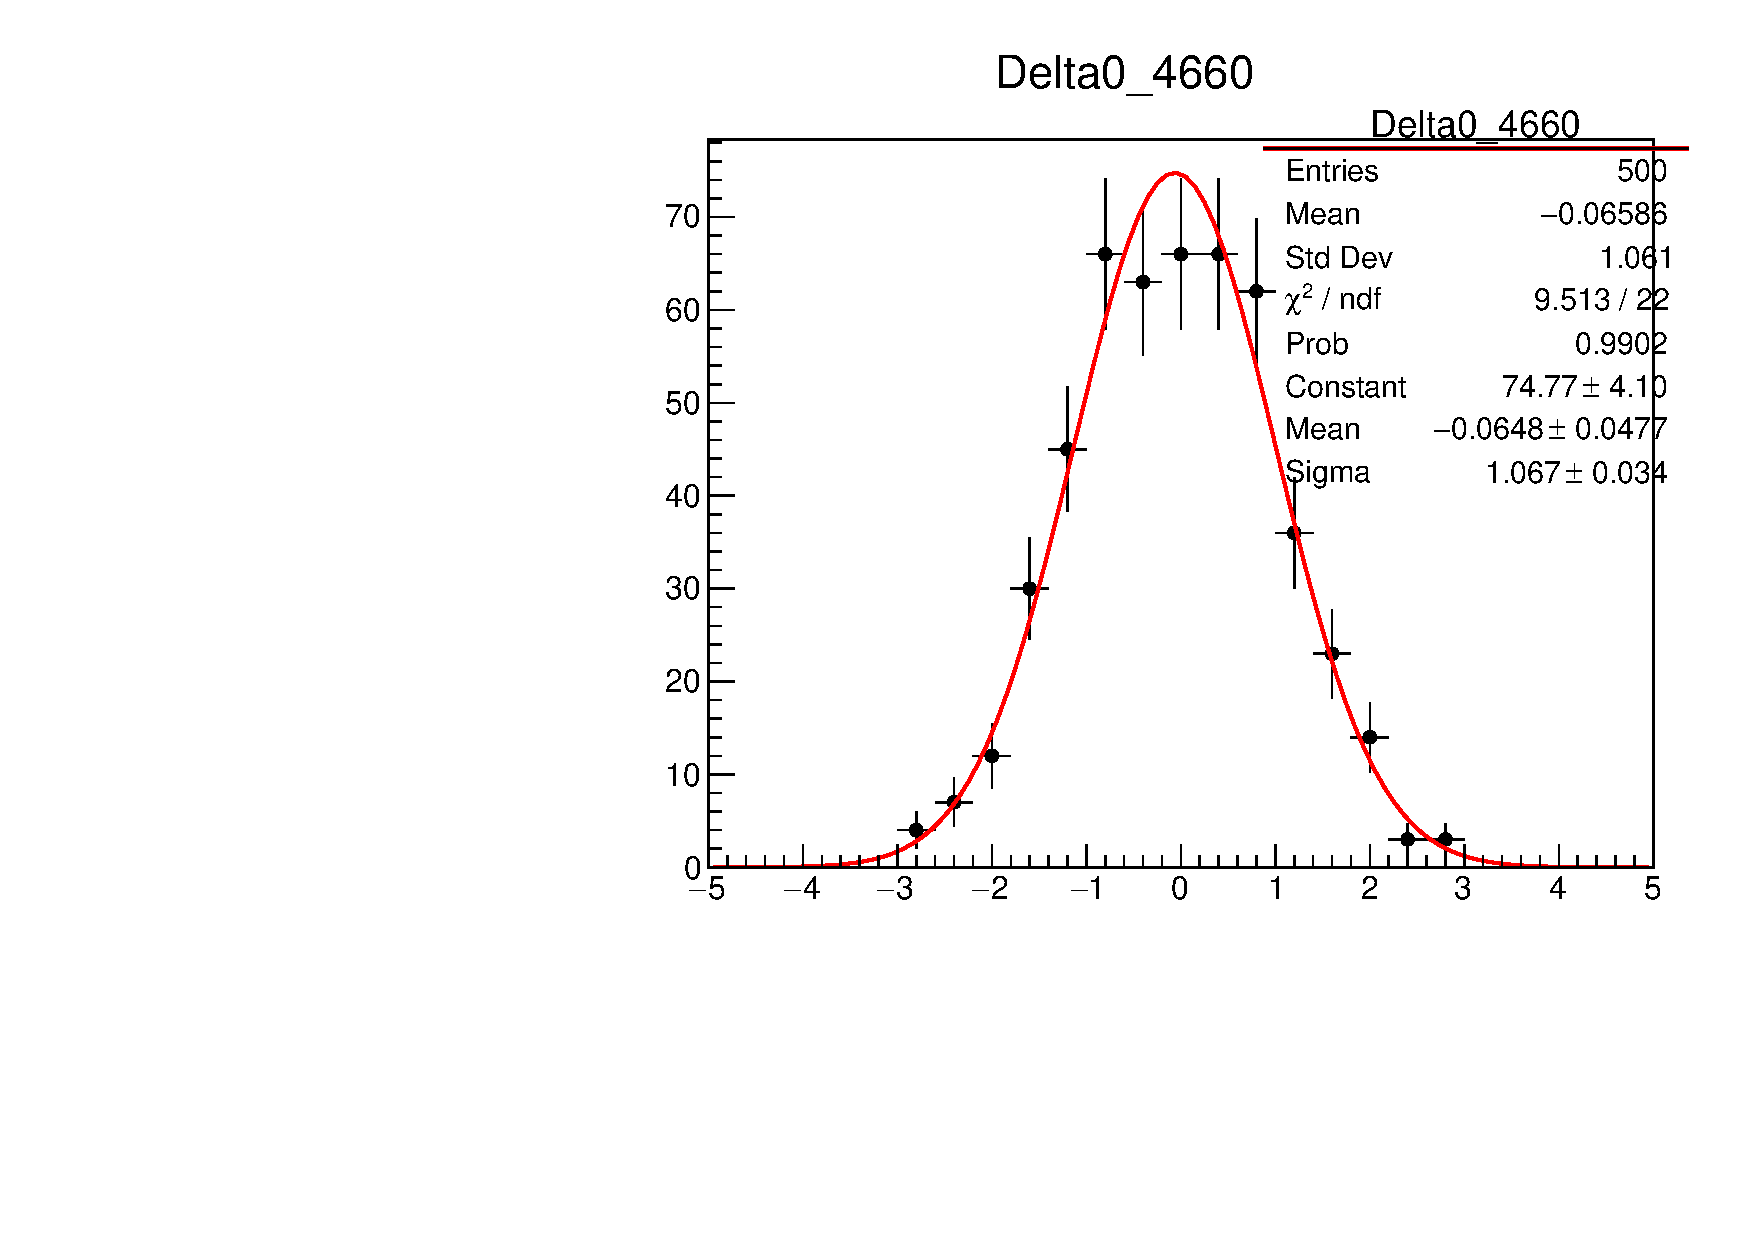
\includegraphics[width=0.24\textwidth]{figure/io_wo_bkg/polarization/pull_polarization_delta0_4660.pdf}
    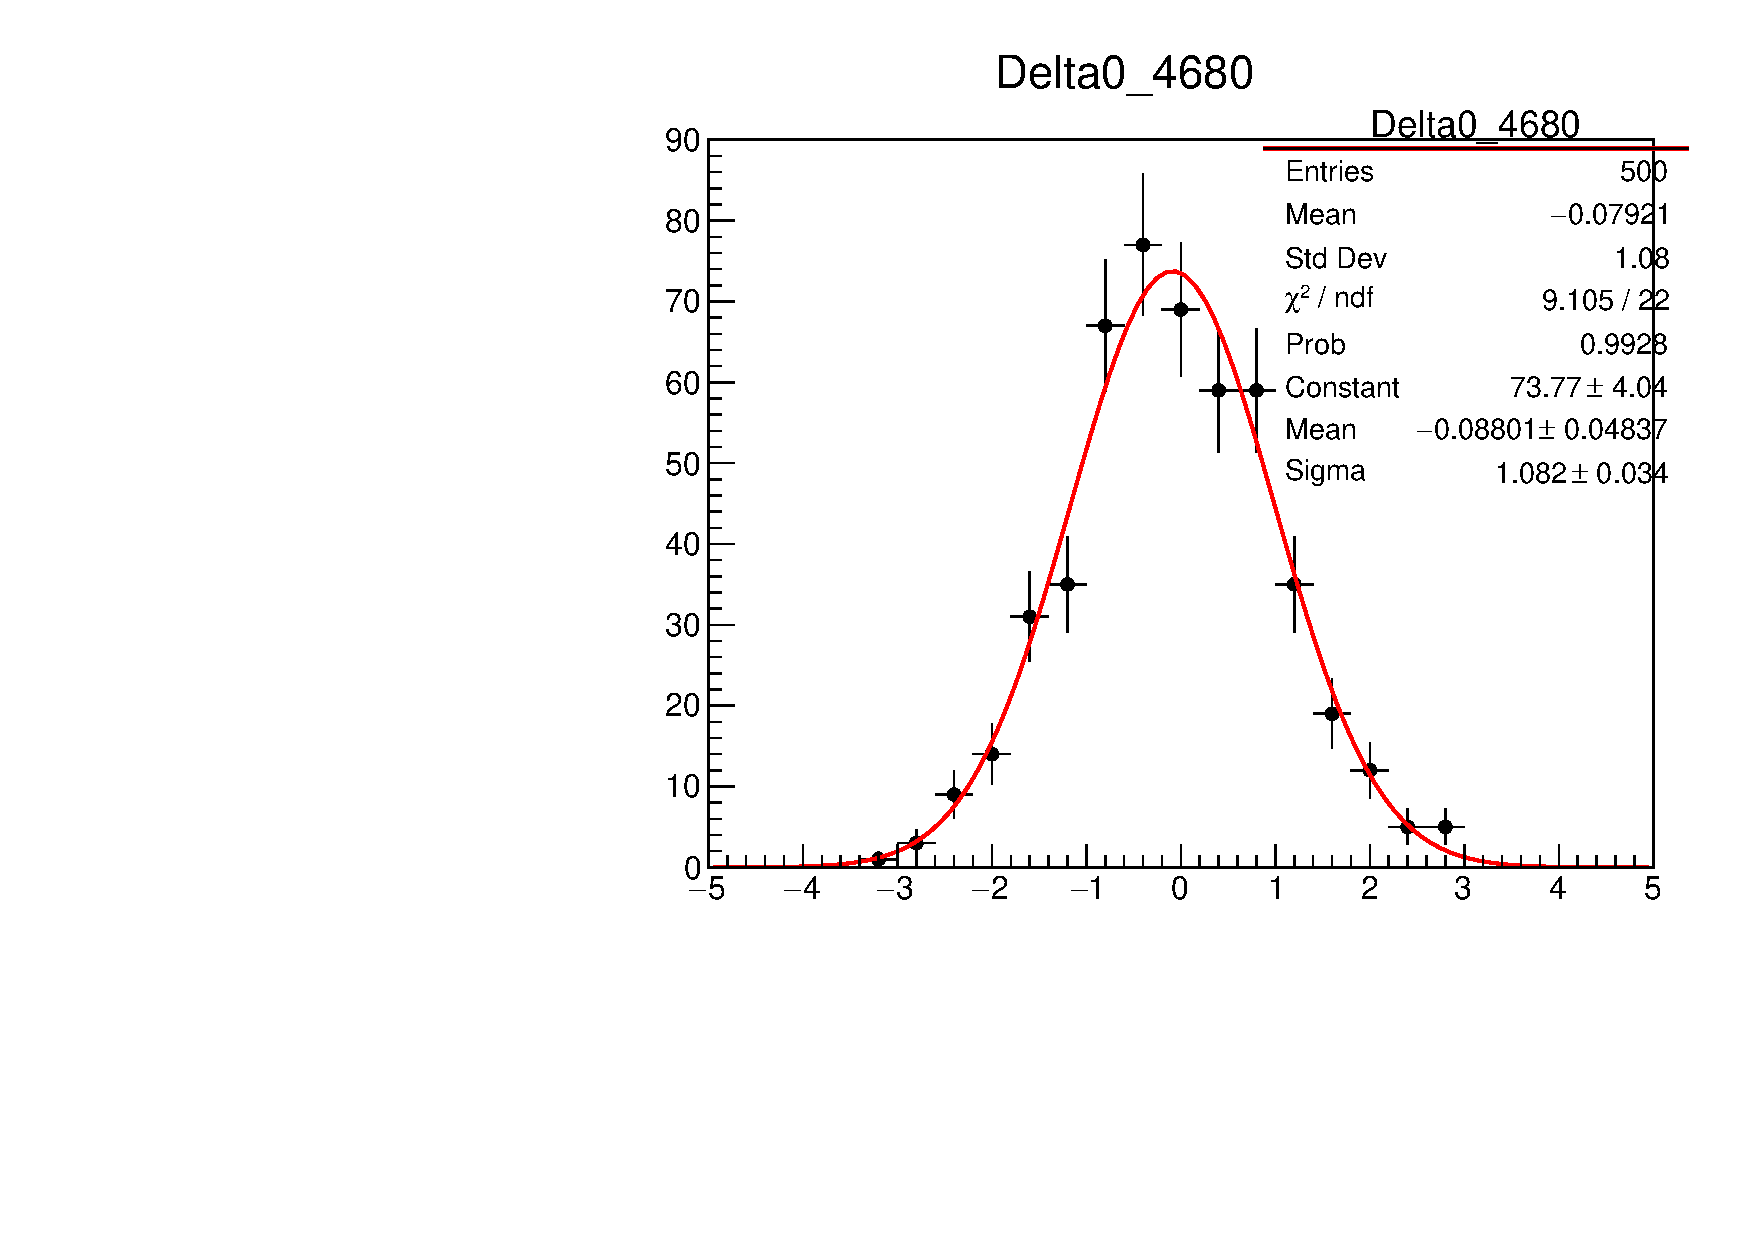
\includegraphics[width=0.24\textwidth]{figure/io_wo_bkg/polarization/pull_polarization_delta0_4680.pdf}
    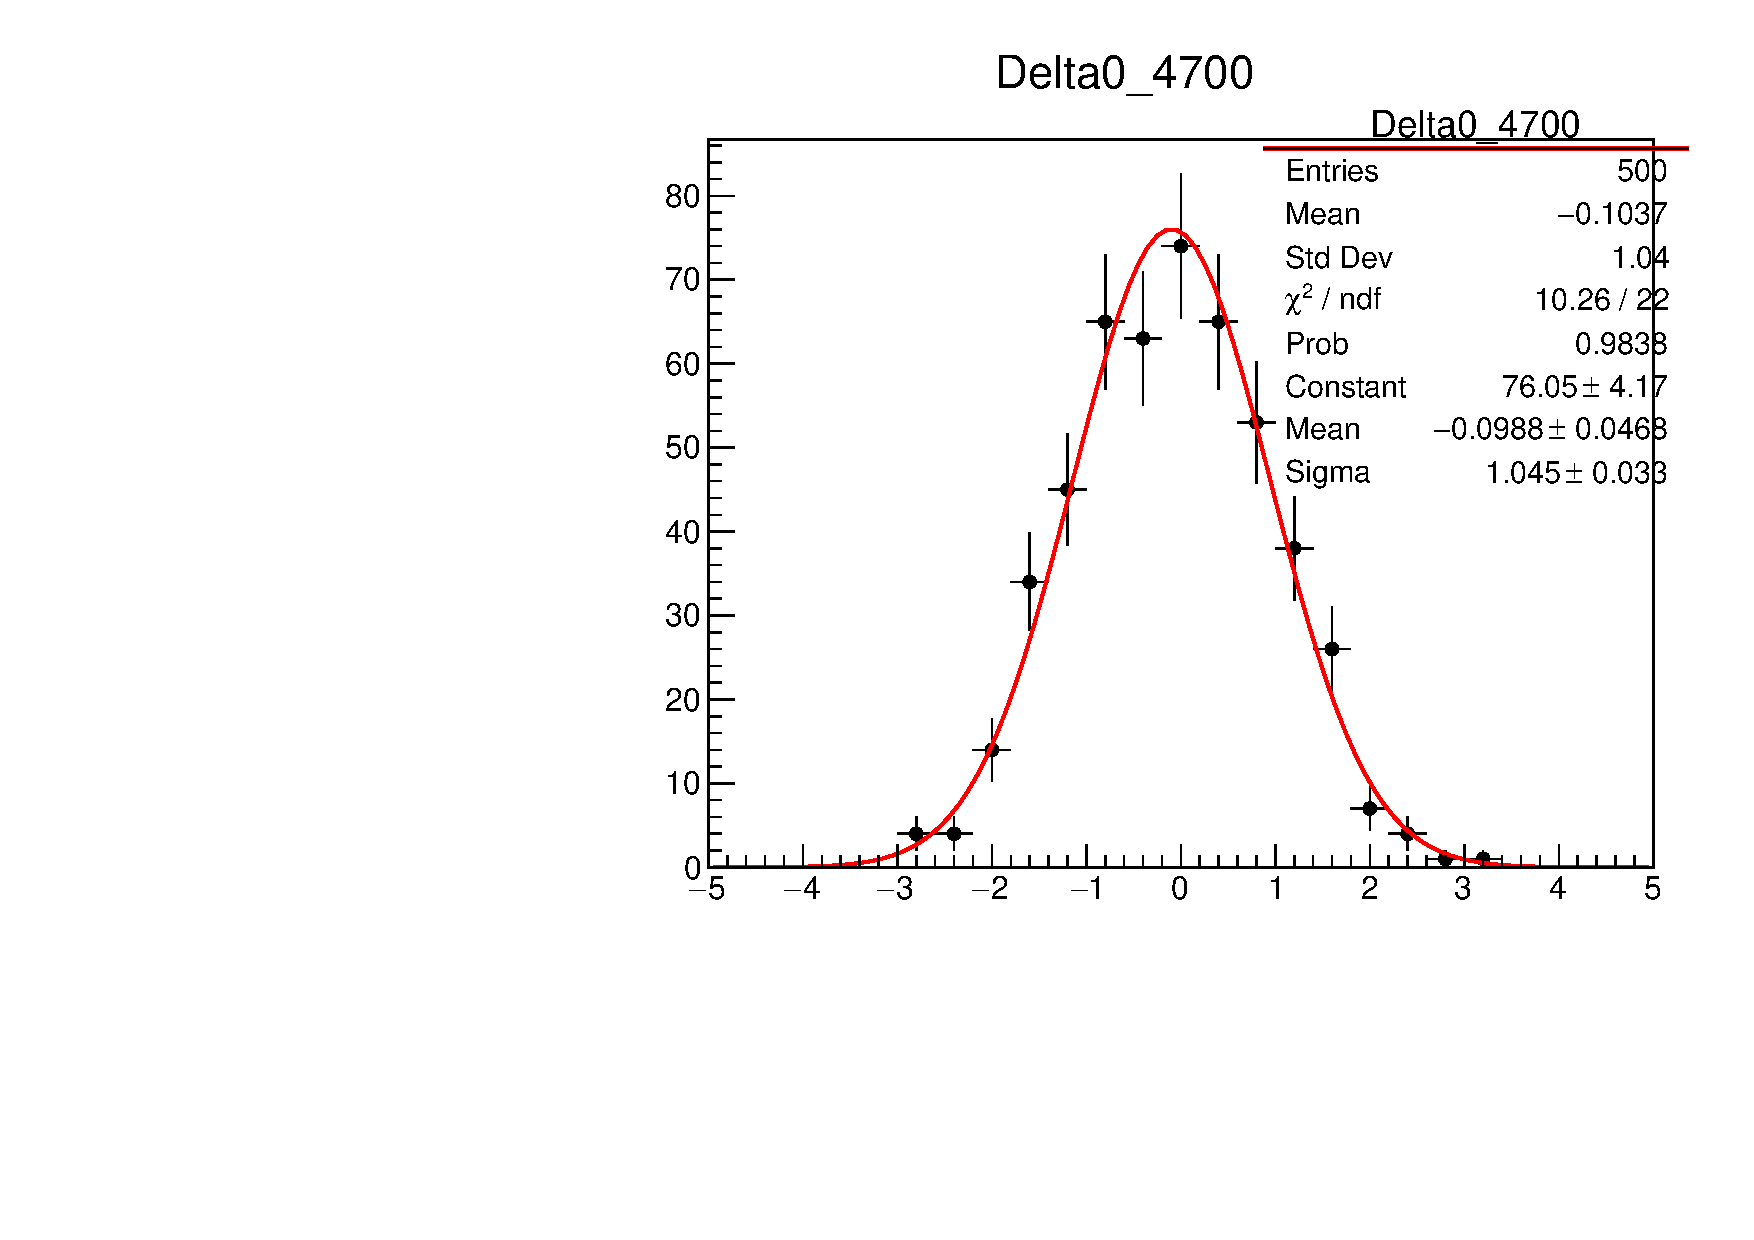
\includegraphics[width=0.24\textwidth]{figure/io_wo_bkg/polarization/pull_polarization_delta0_4700.pdf}
    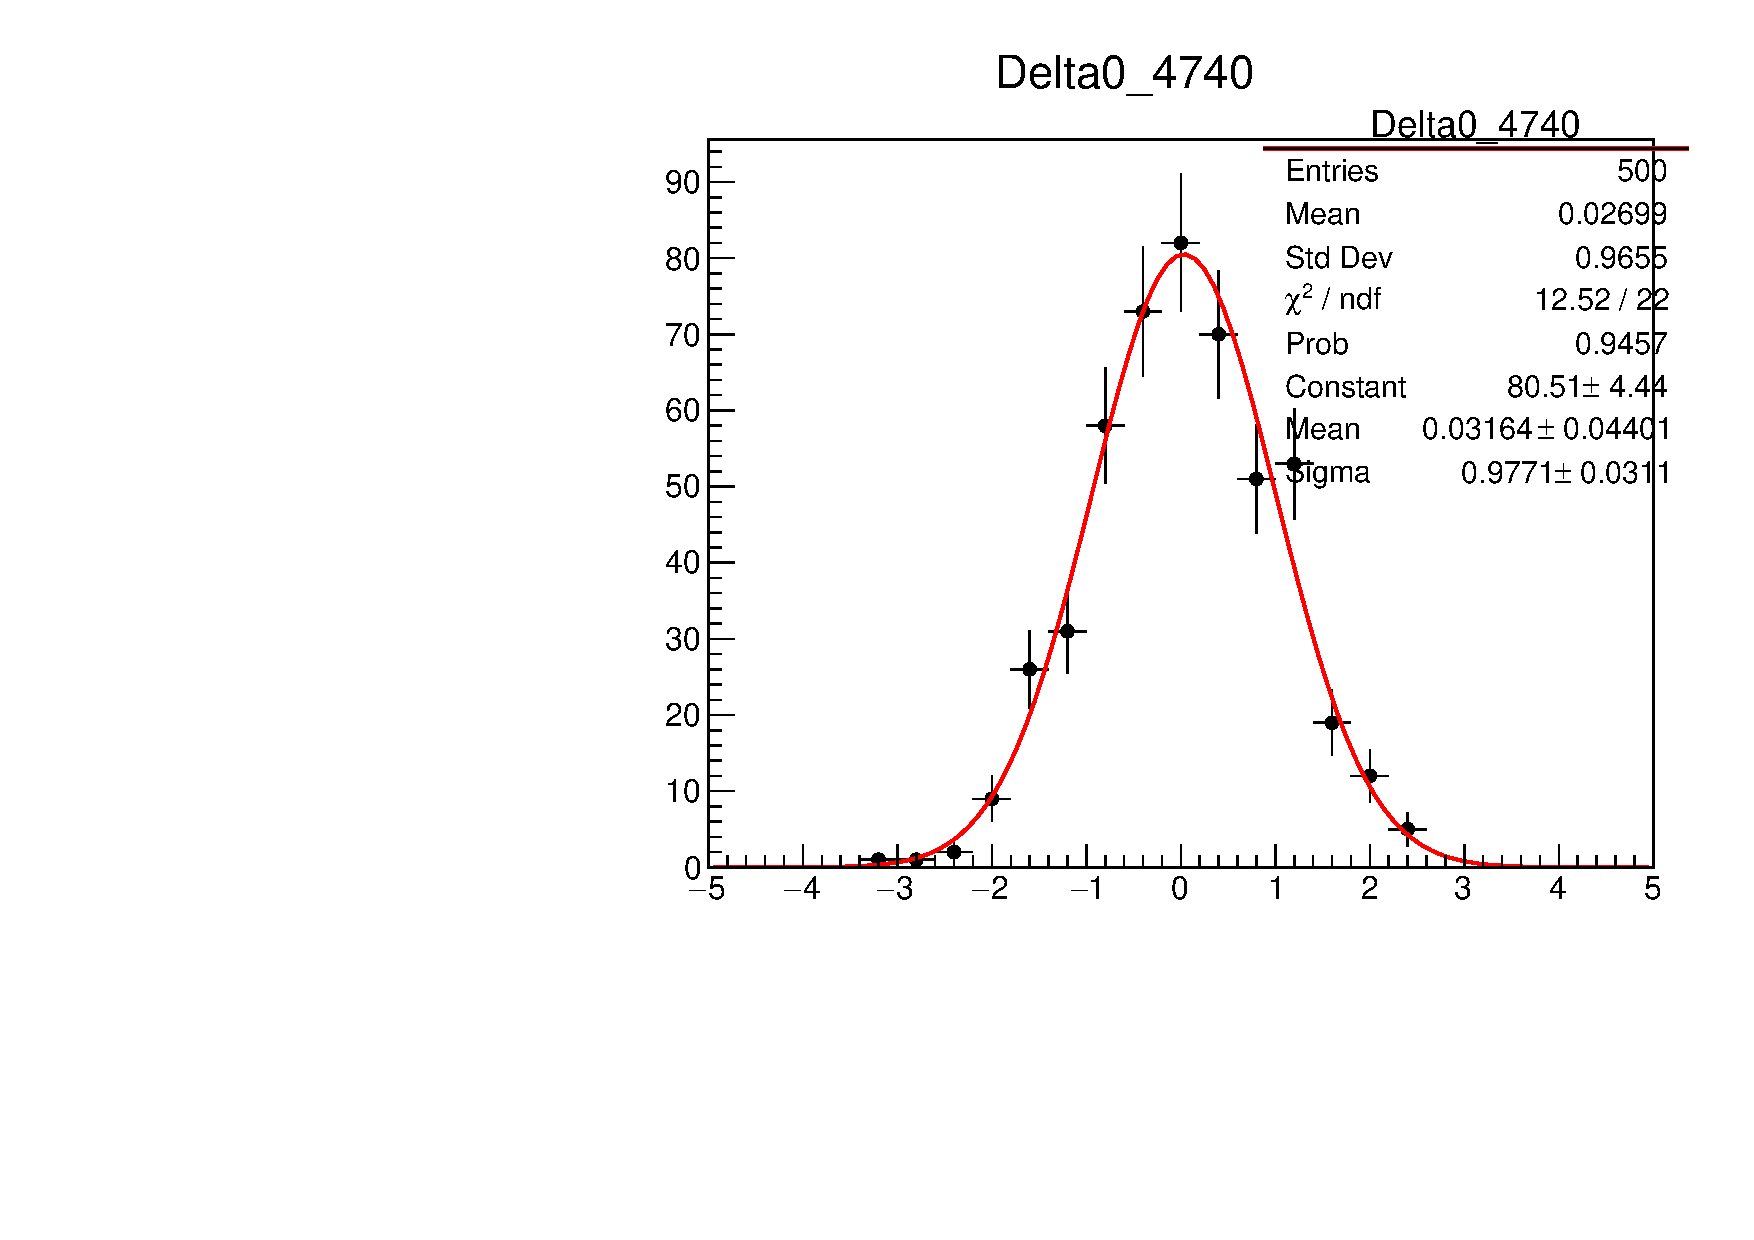
\includegraphics[width=0.24\textwidth]{figure/io_wo_bkg/polarization/pull_polarization_delta0_4740.pdf}
    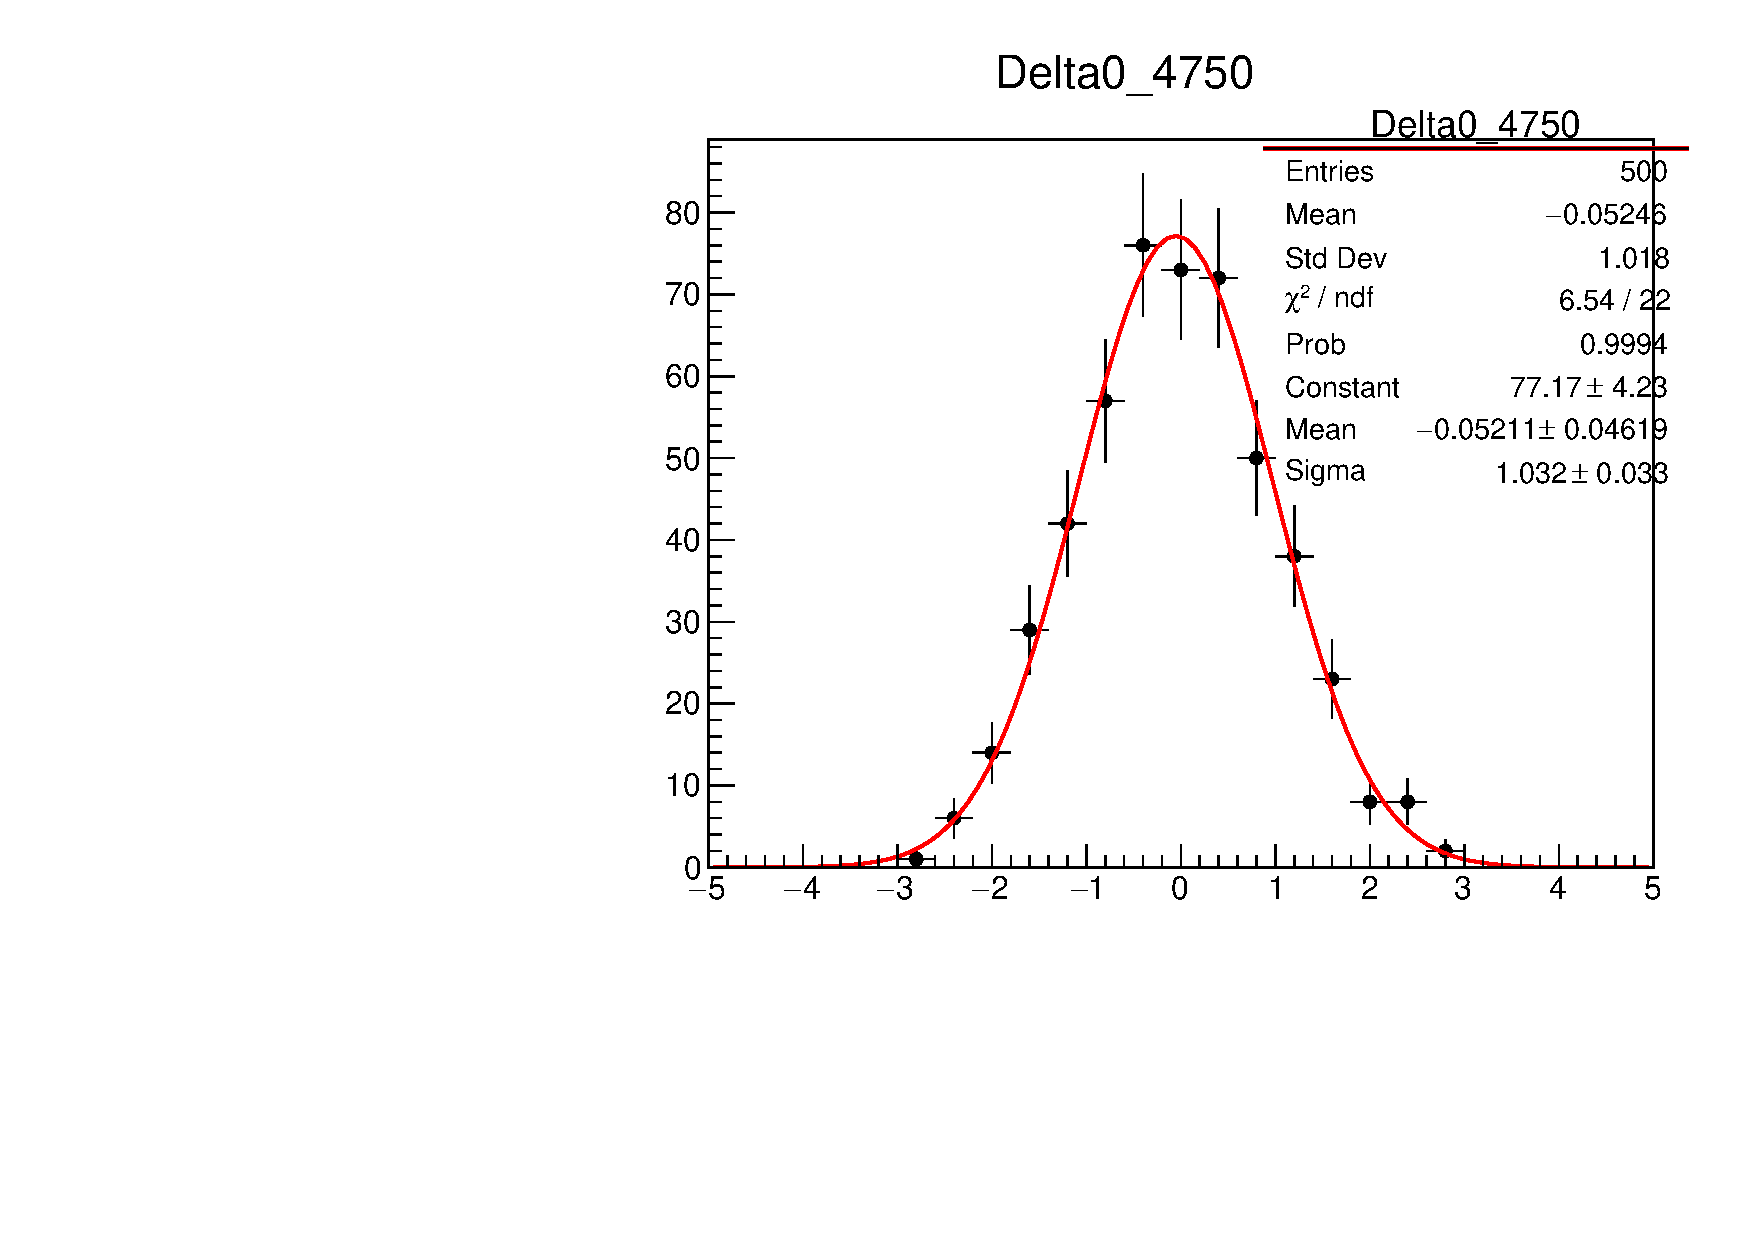
\includegraphics[width=0.24\textwidth]{figure/io_wo_bkg/polarization/pull_polarization_delta0_4750.pdf}
    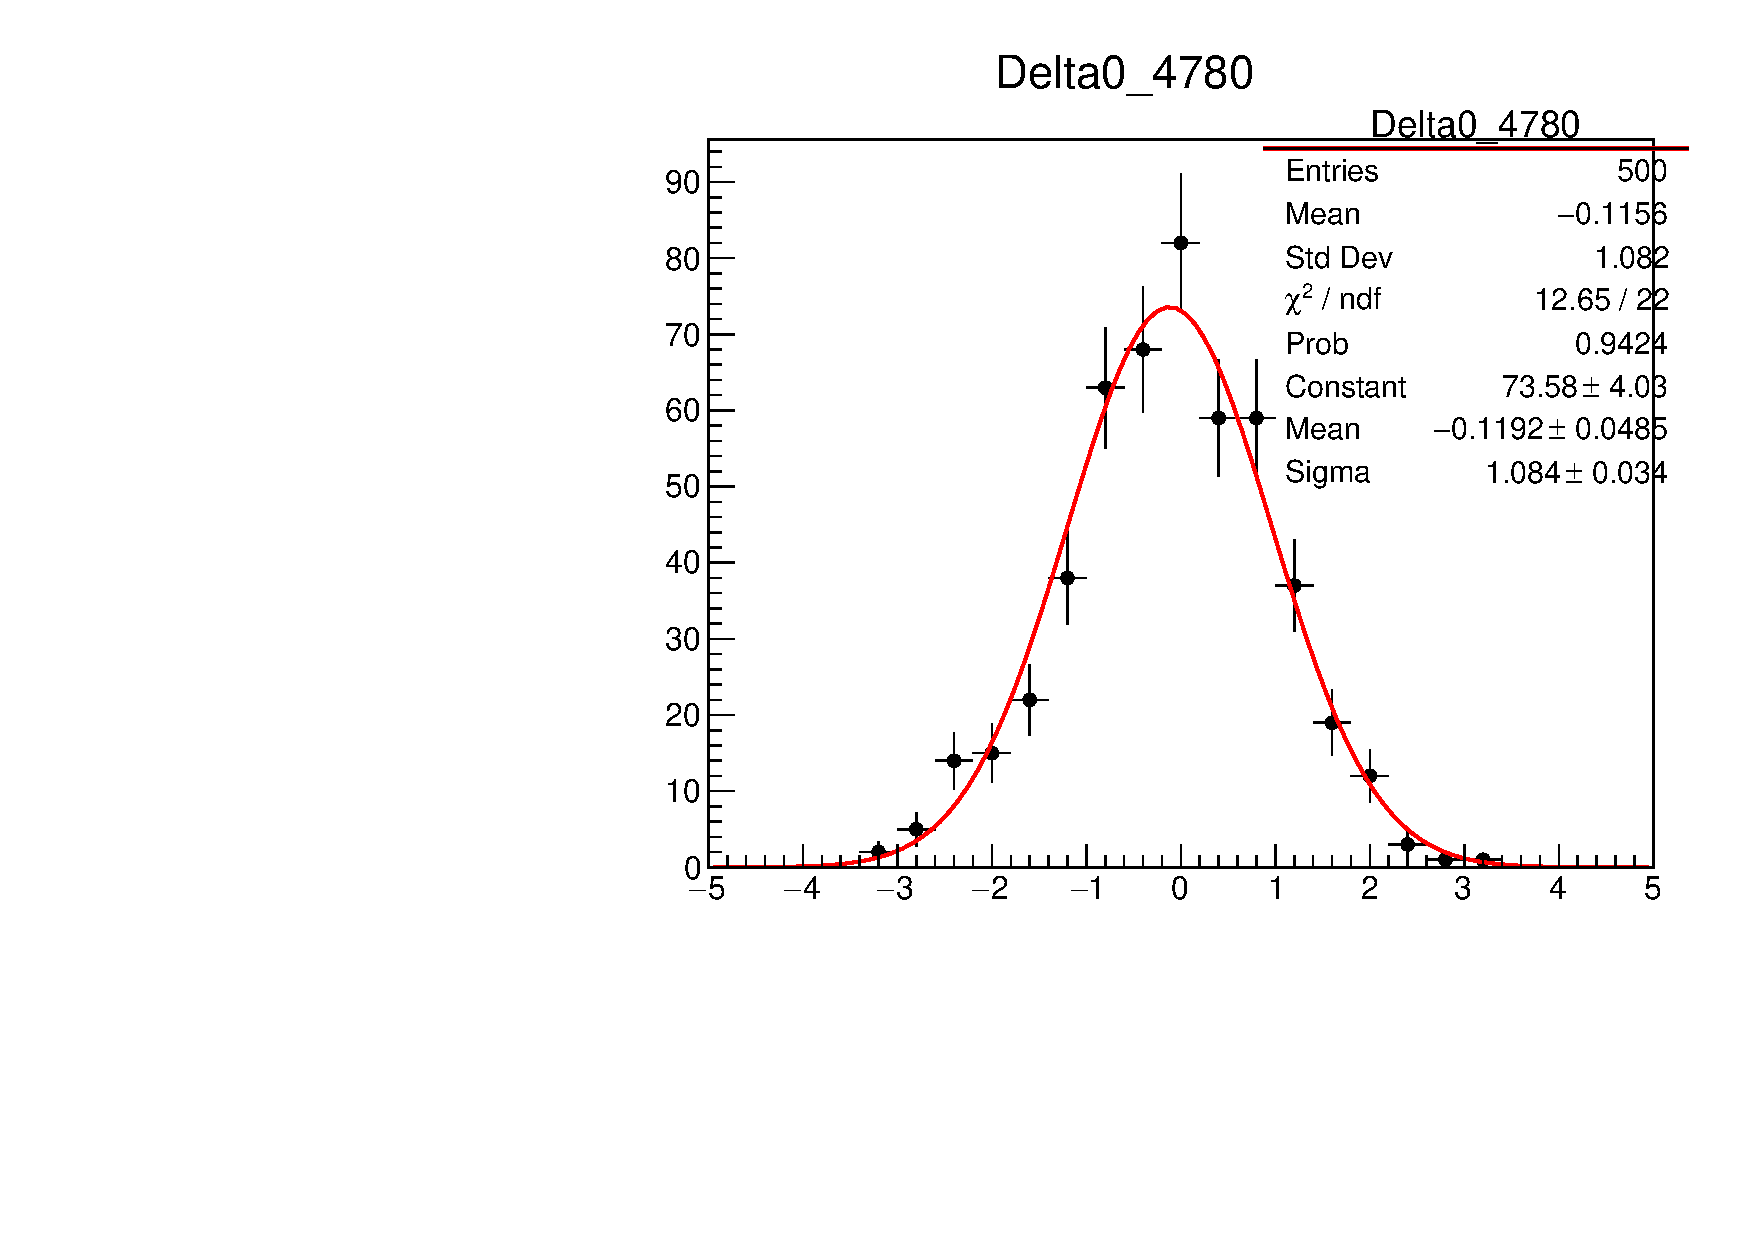
\includegraphics[width=0.24\textwidth]{figure/io_wo_bkg/polarization/pull_polarization_delta0_4780.pdf}
    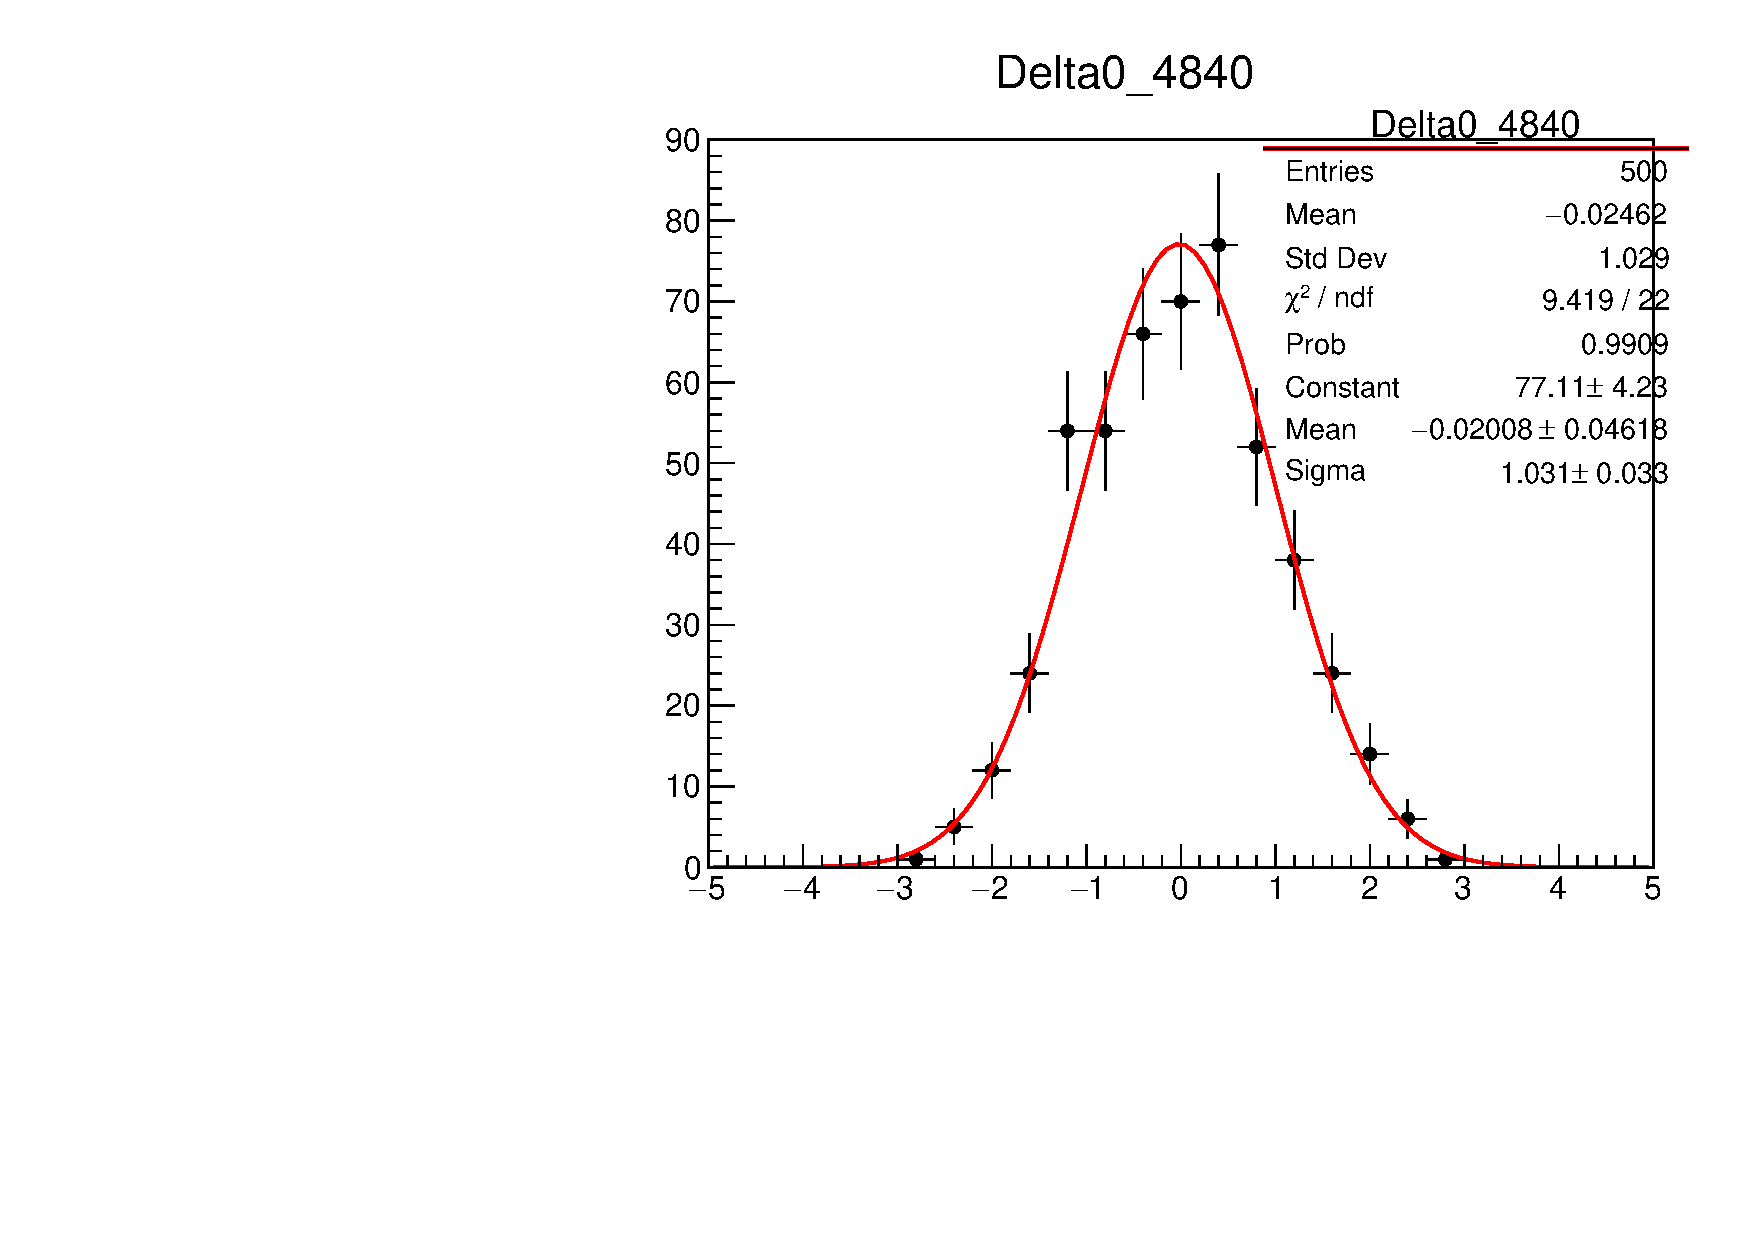
\includegraphics[width=0.24\textwidth]{figure/io_wo_bkg/polarization/pull_polarization_delta0_4840.pdf}
    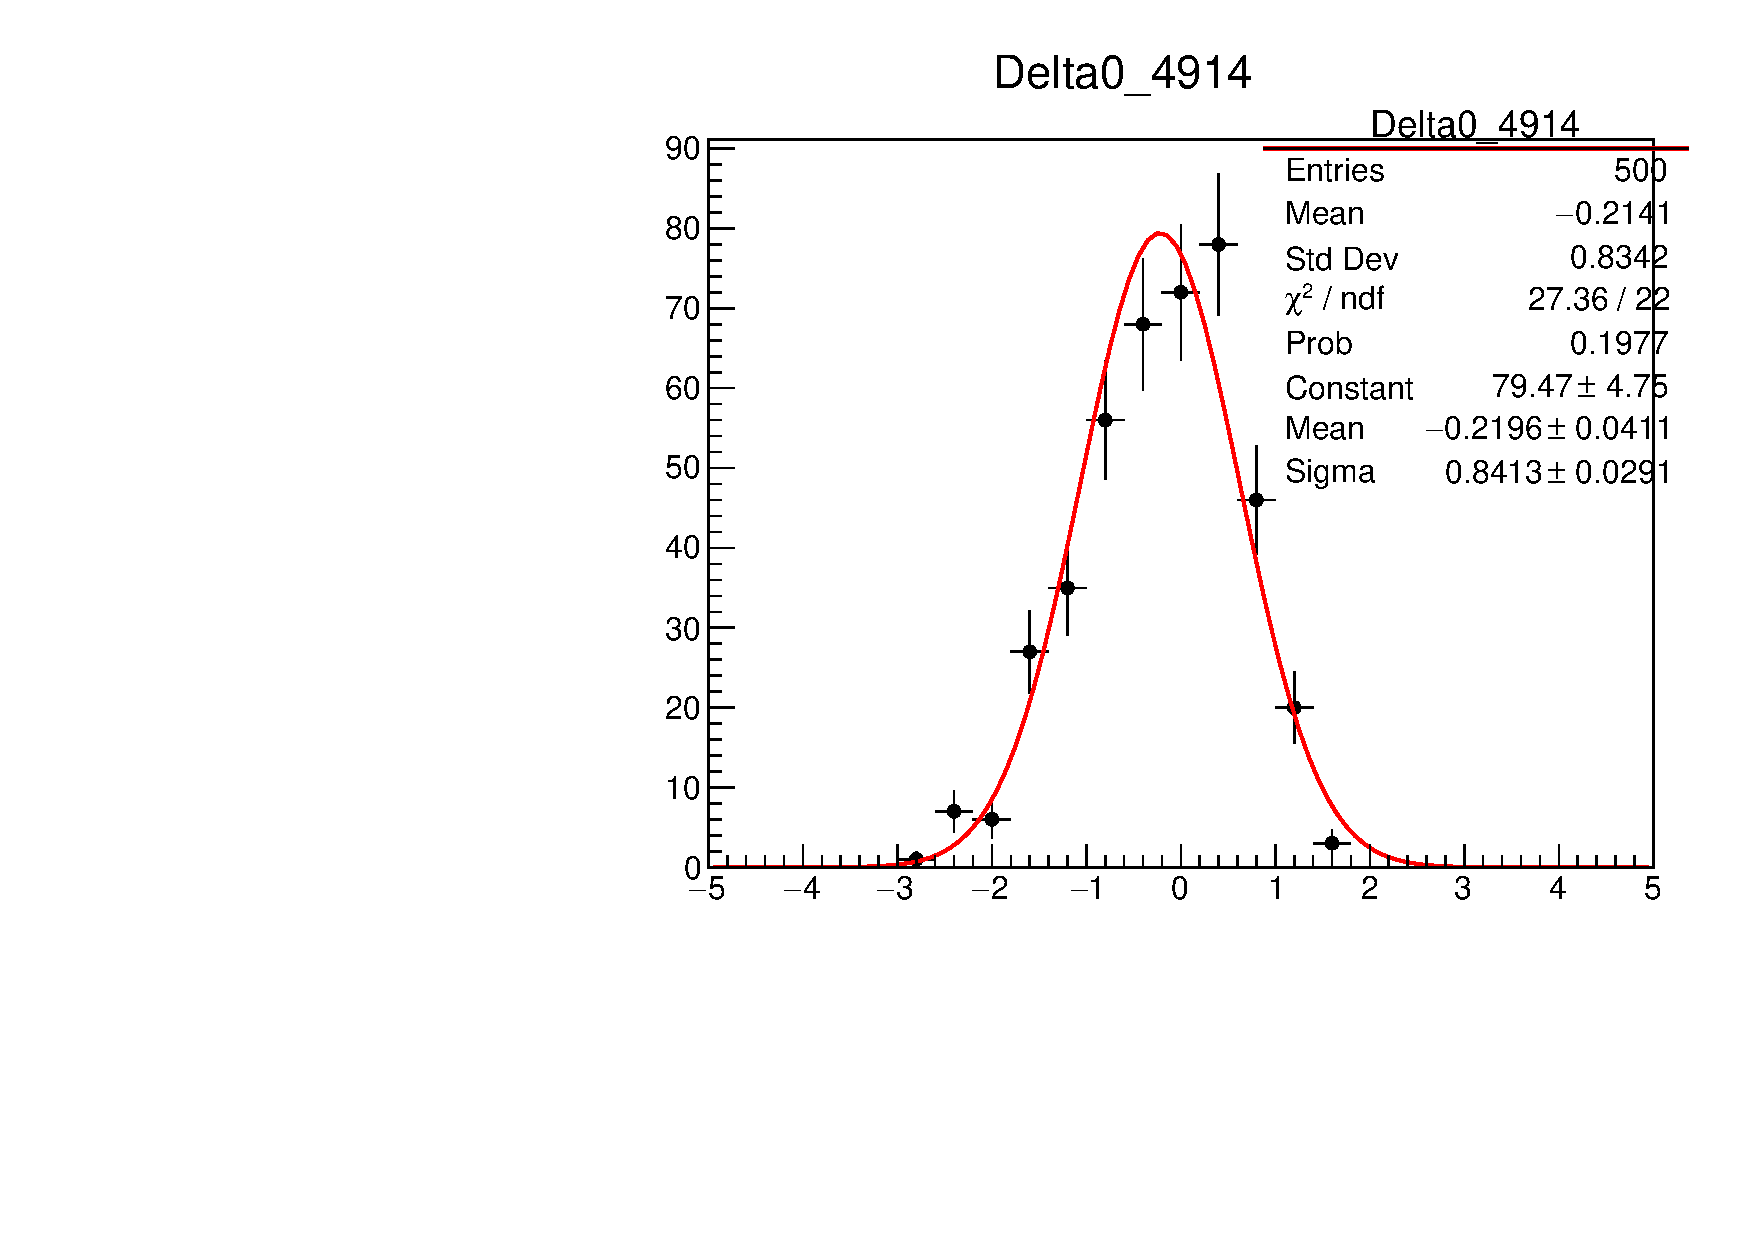
\includegraphics[width=0.24\textwidth]{figure/io_wo_bkg/polarization/pull_polarization_delta0_4914.pdf}
    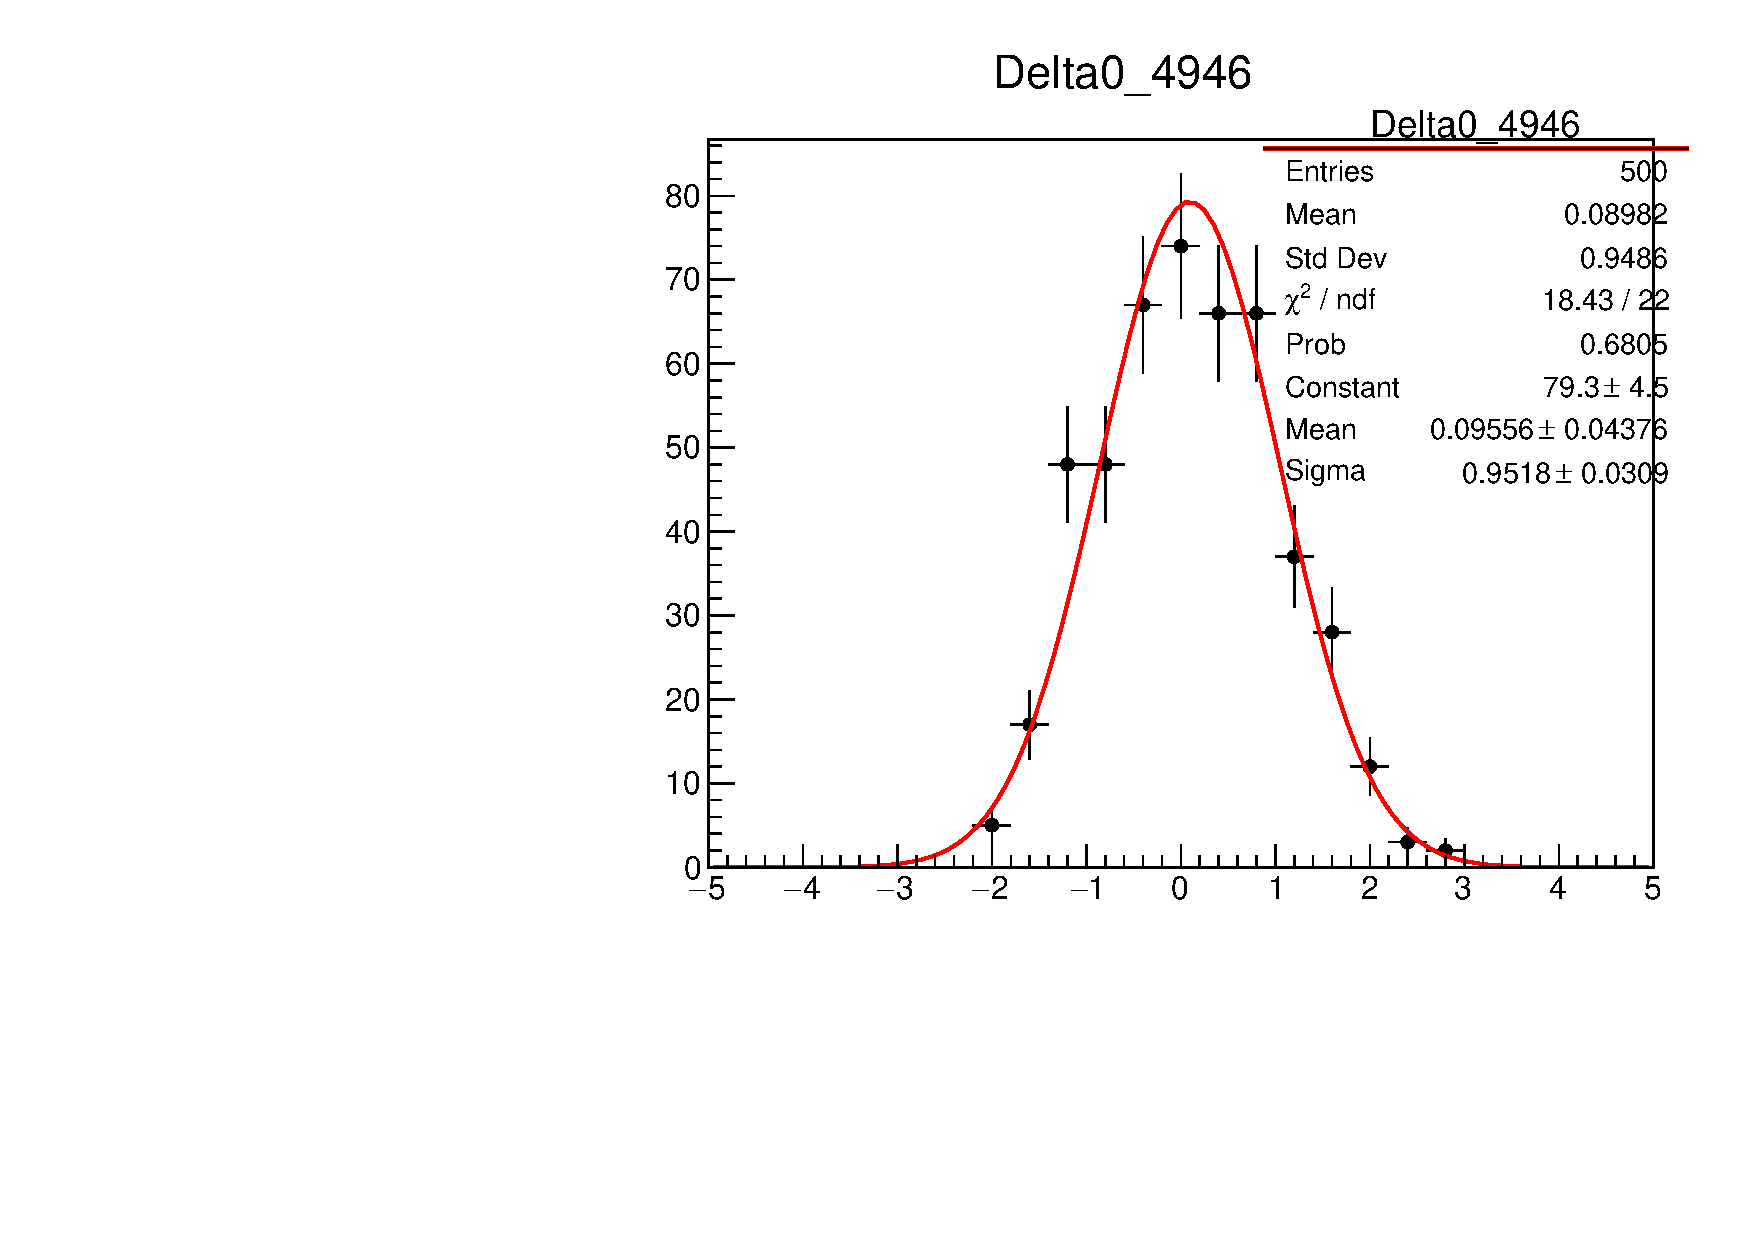
\includegraphics[width=0.24\textwidth]{figure/io_wo_bkg/polarization/pull_polarization_delta0_4946.pdf}
    \caption{Pull distributions of $\sin\Delta_0$ for each energy point.}
\label{fig:io_wo_bkg_pull_delta0}
\end{figure}

\begin{figure}[h]\centering
    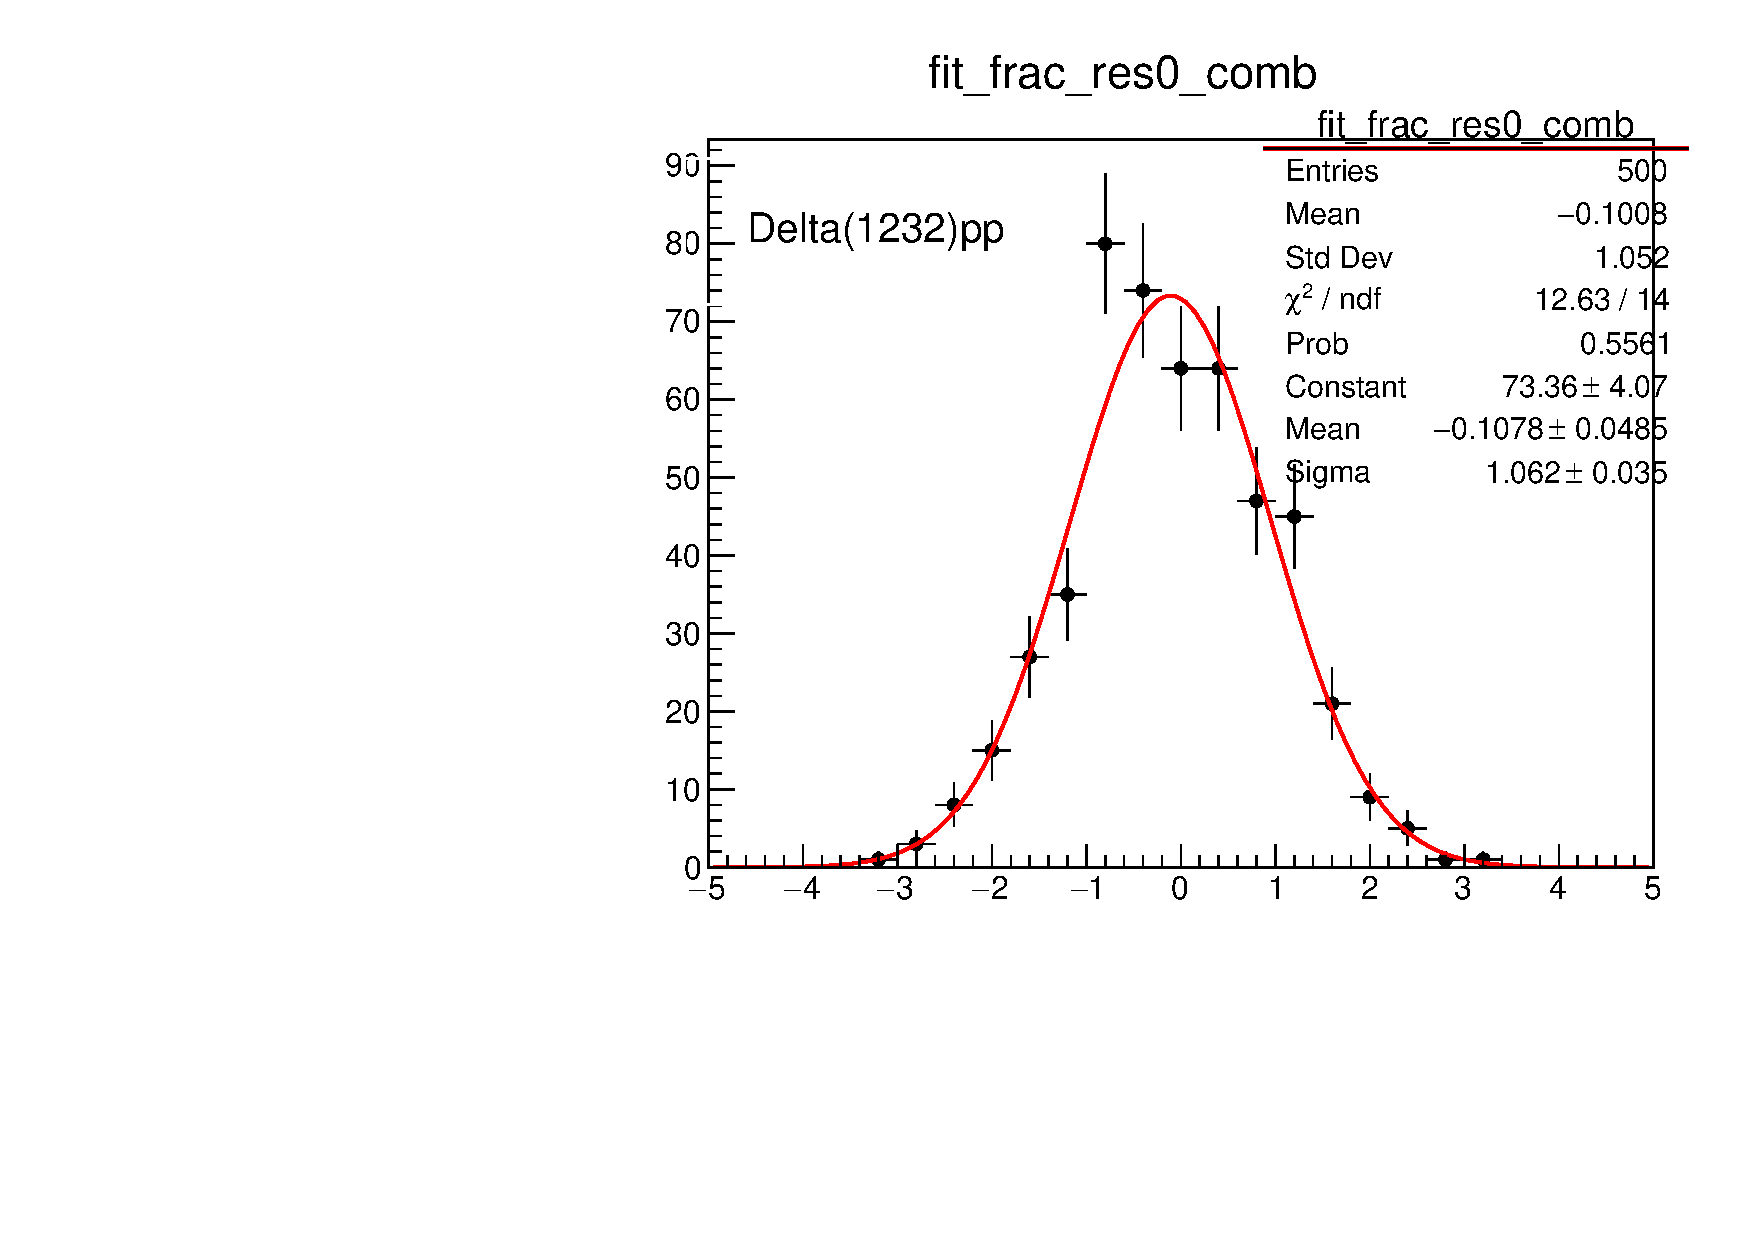
\includegraphics[width=0.24\textwidth]{figure/io_wo_bkg/fitfrac/pull_fitfrac_res0_comb.pdf}
    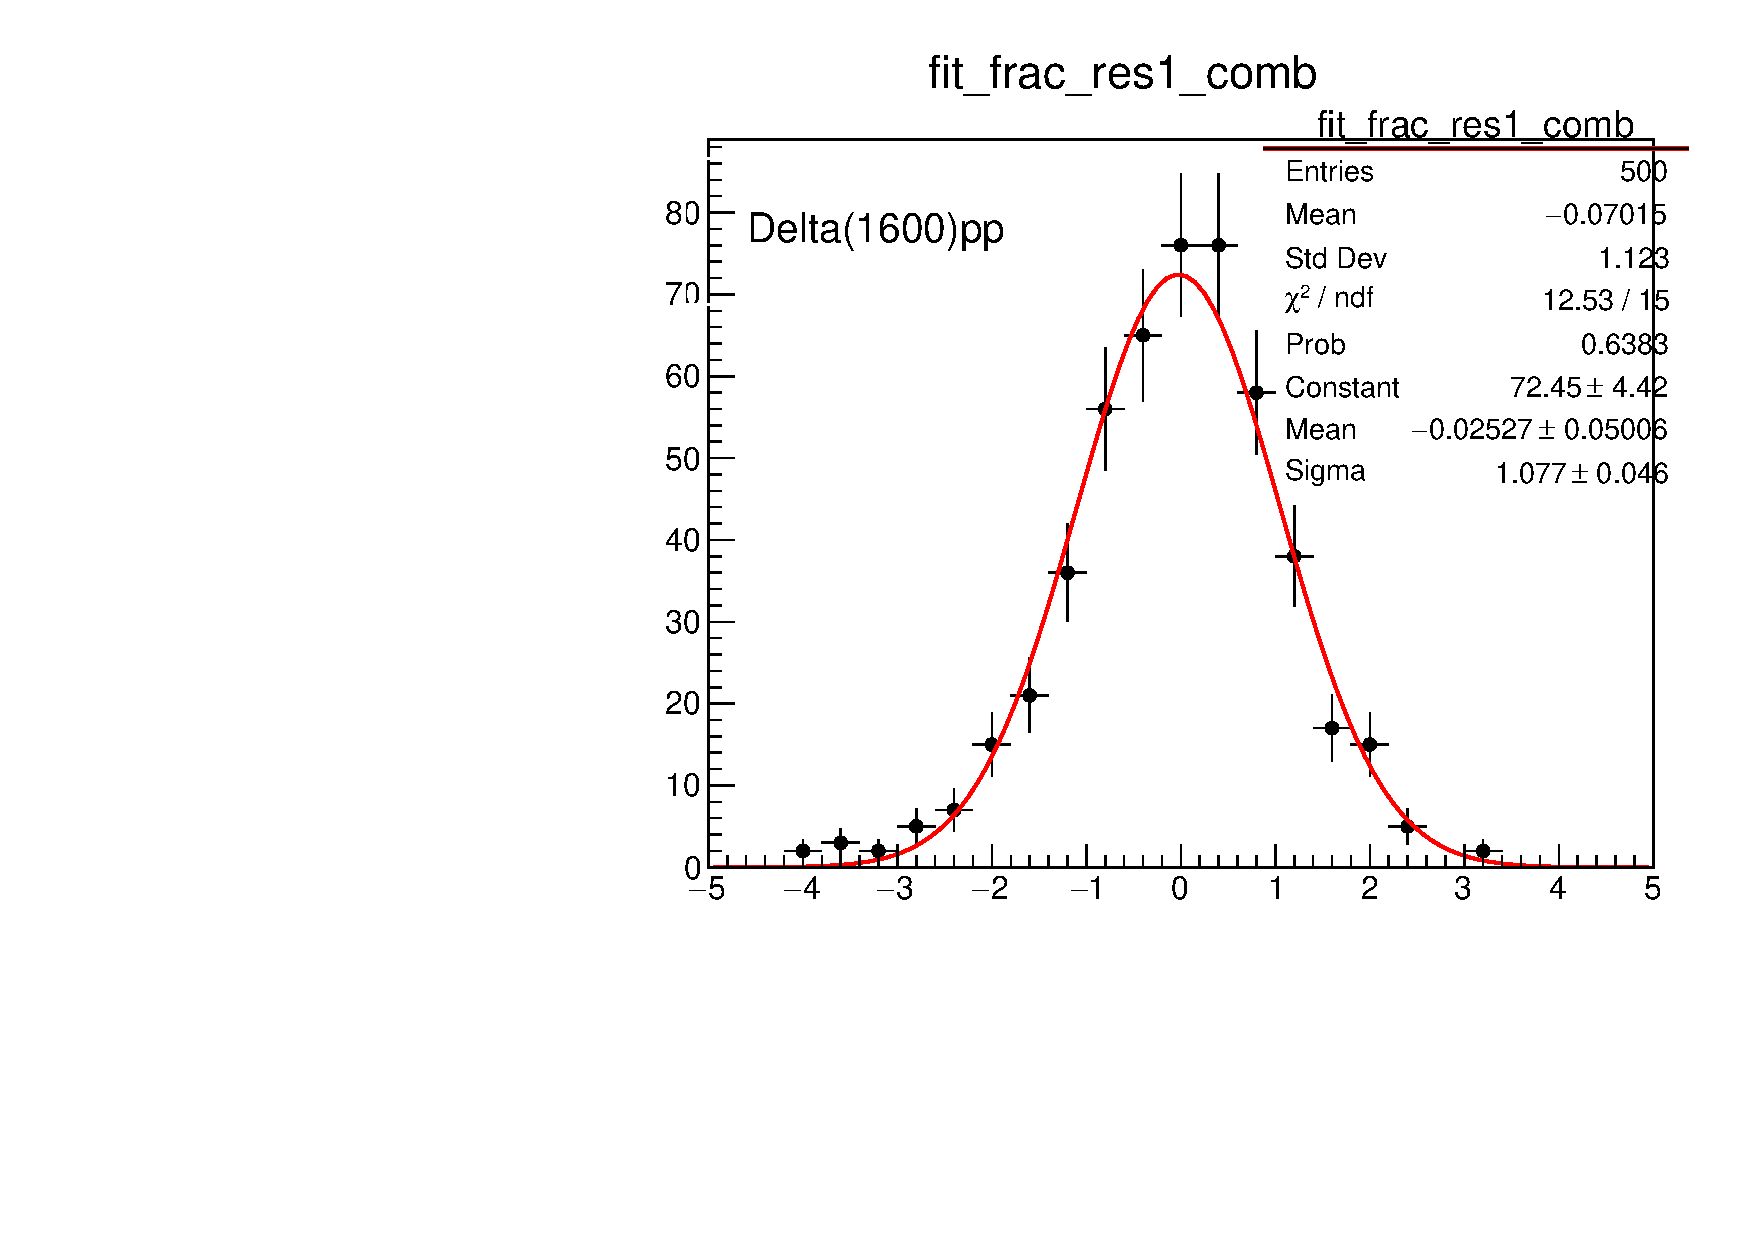
\includegraphics[width=0.24\textwidth]{figure/io_wo_bkg/fitfrac/pull_fitfrac_res1_comb.pdf}
    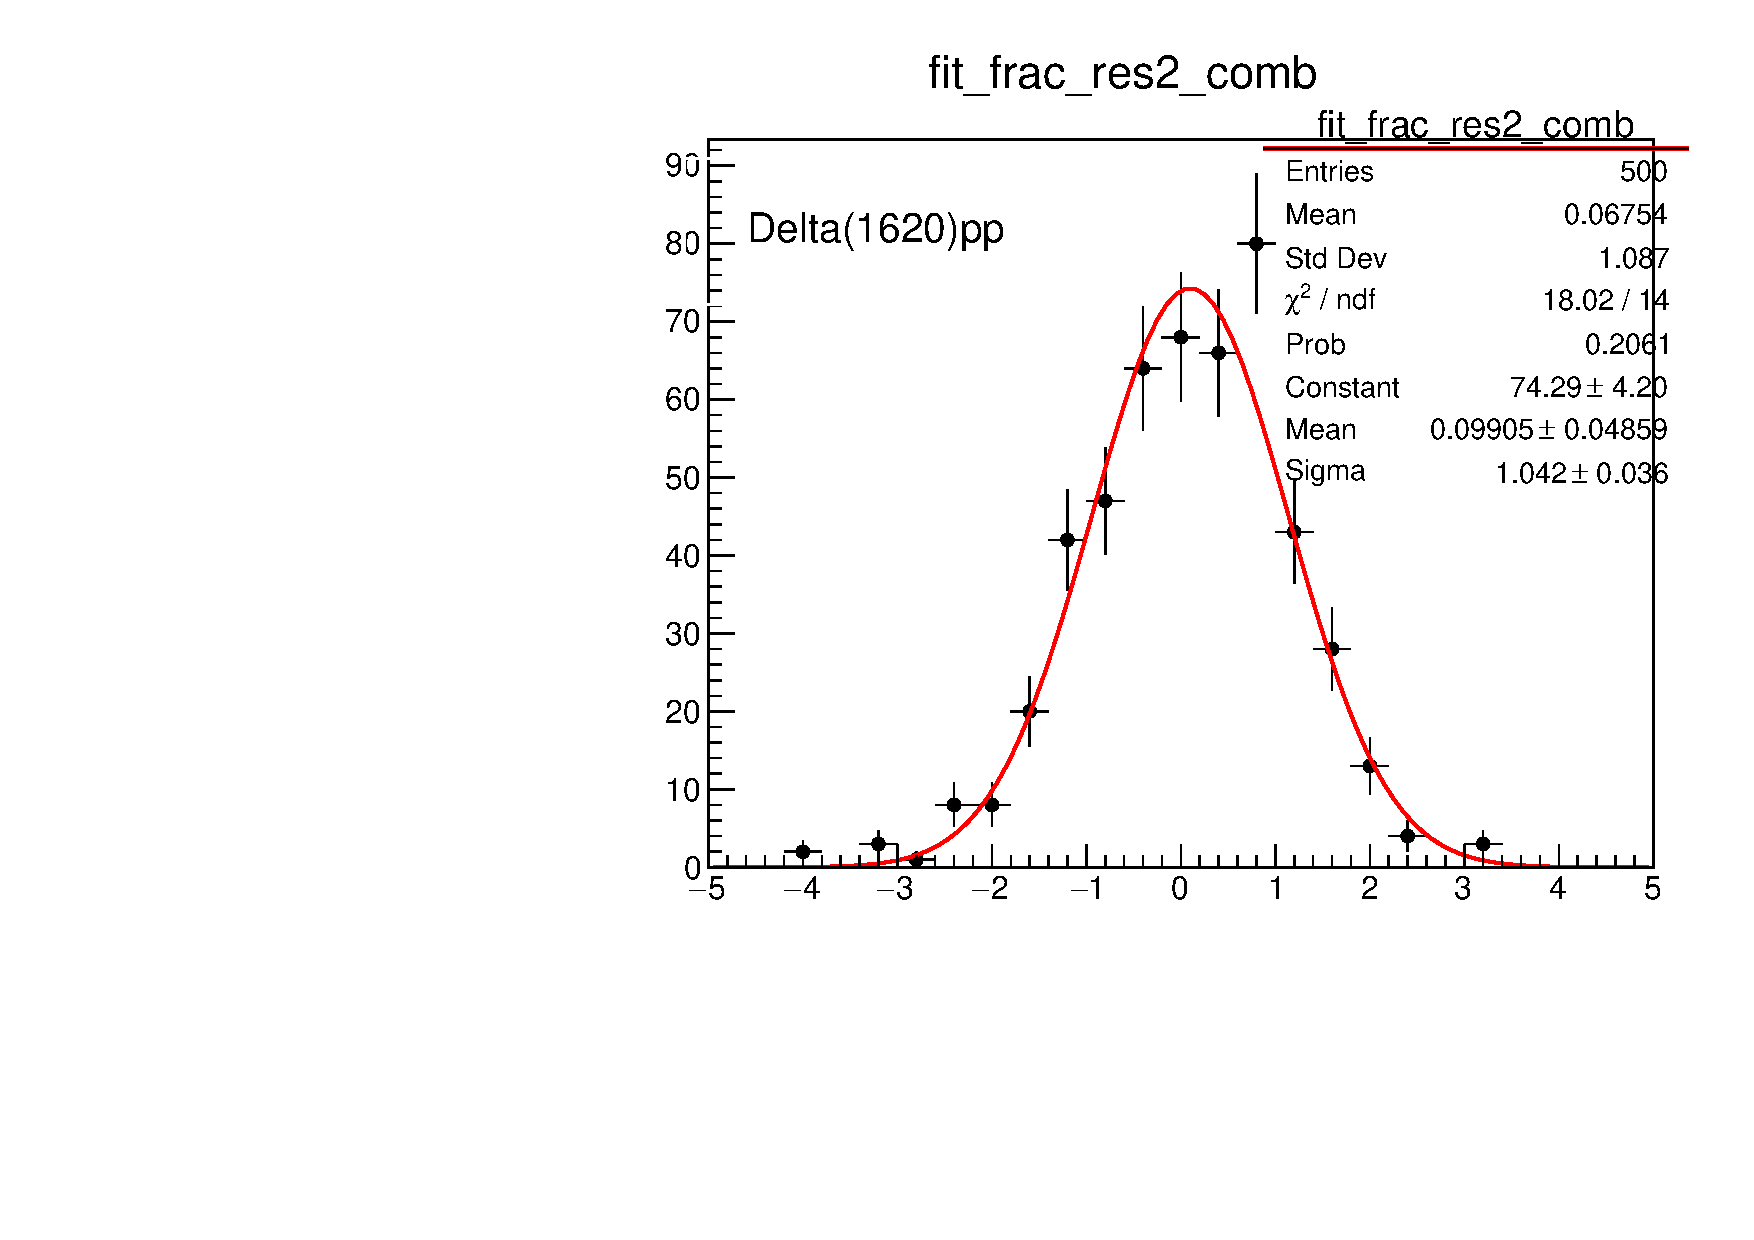
\includegraphics[width=0.24\textwidth]{figure/io_wo_bkg/fitfrac/pull_fitfrac_res2_comb.pdf}
    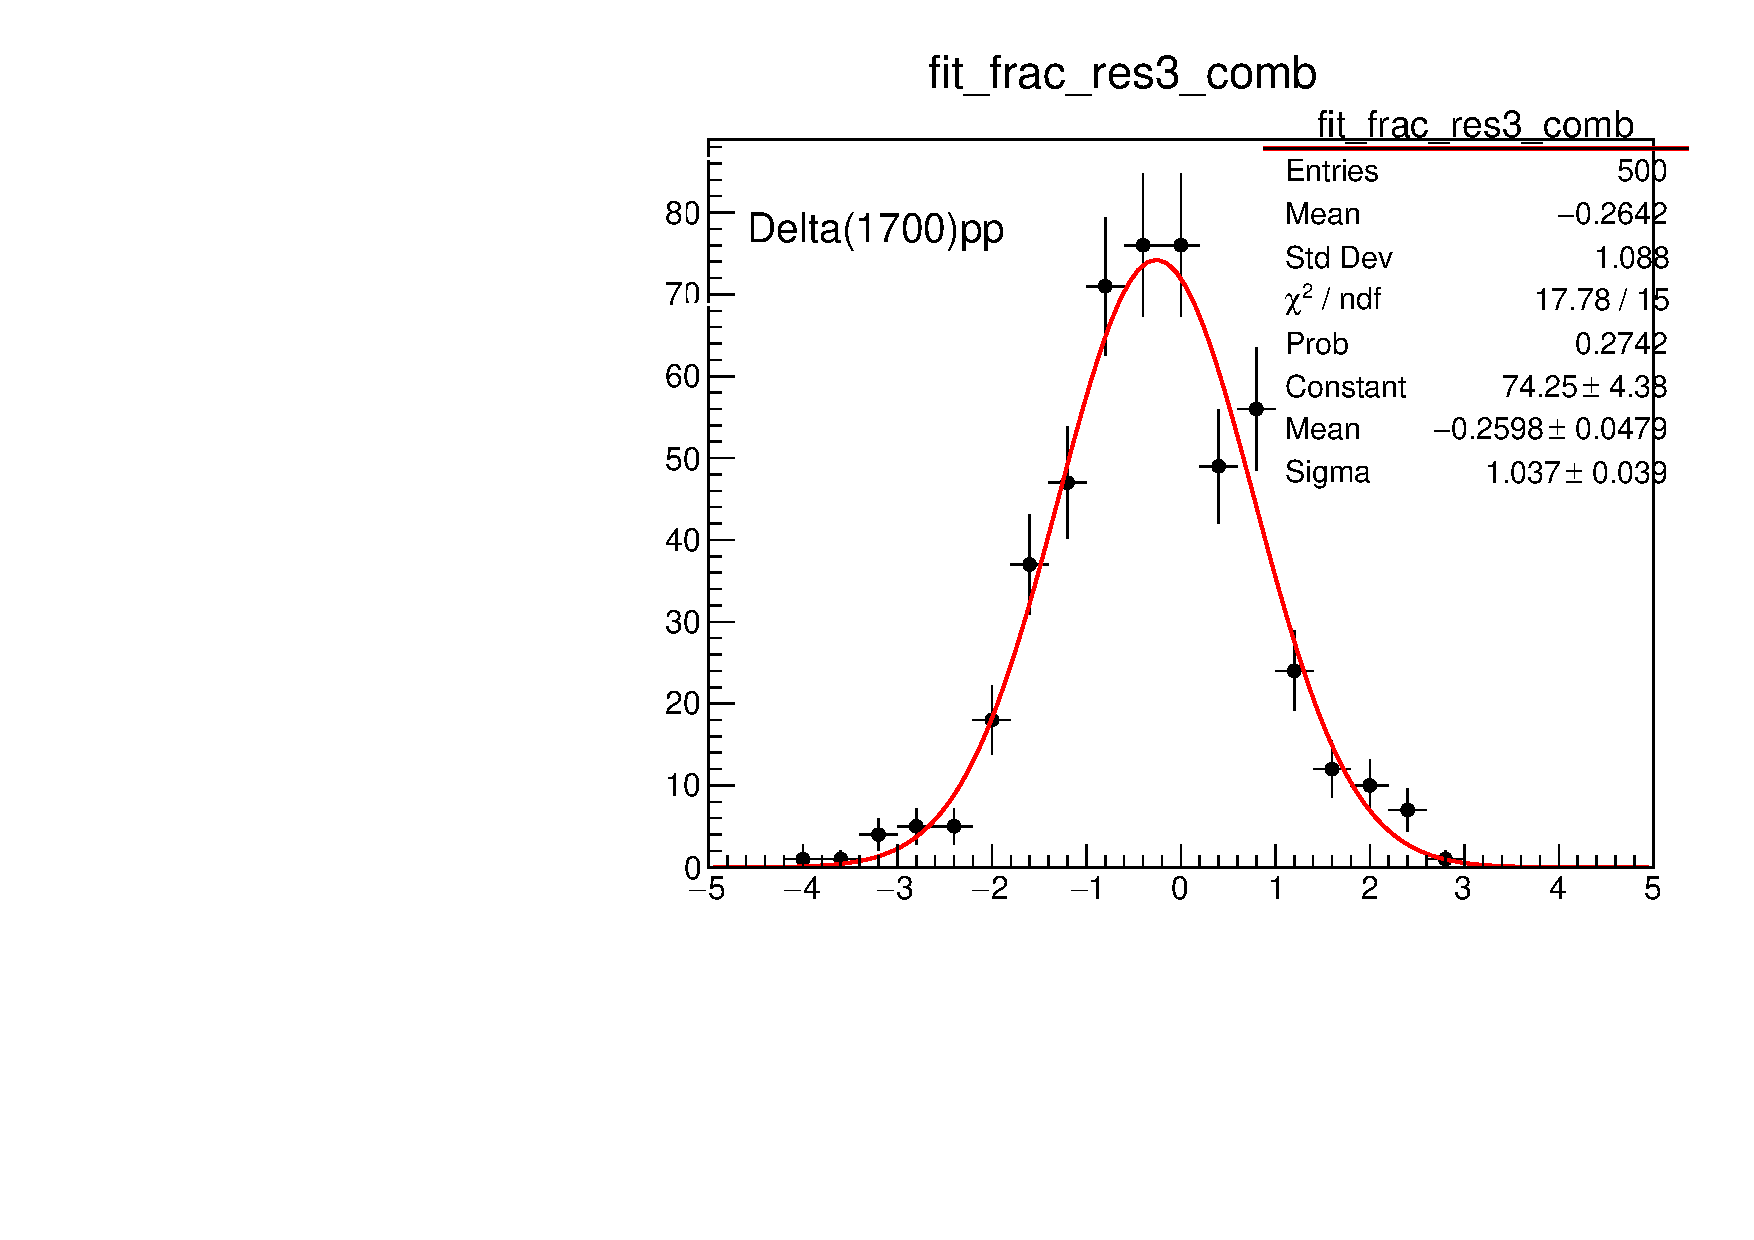
\includegraphics[width=0.24\textwidth]{figure/io_wo_bkg/fitfrac/pull_fitfrac_res3_comb.pdf}
    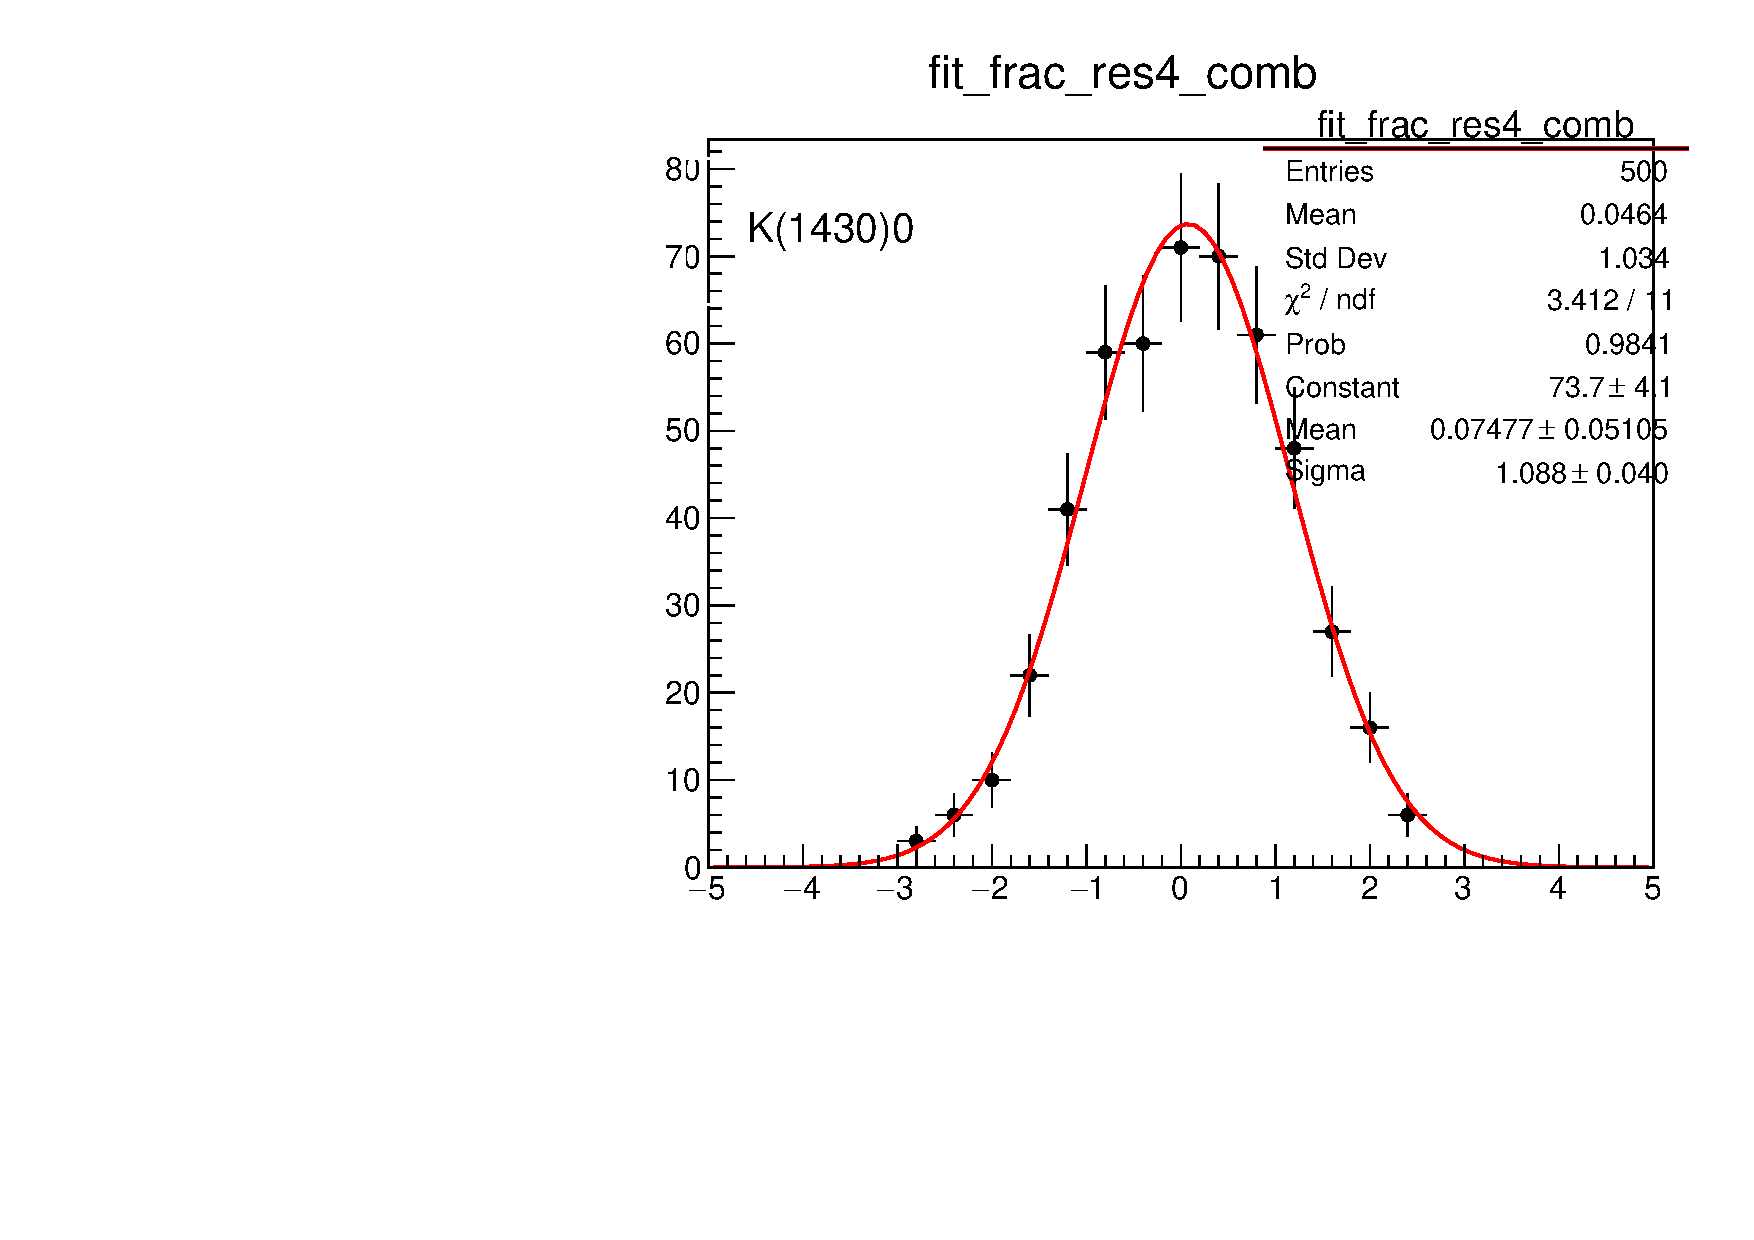
\includegraphics[width=0.24\textwidth]{figure/io_wo_bkg/fitfrac/pull_fitfrac_res4_comb.pdf}
    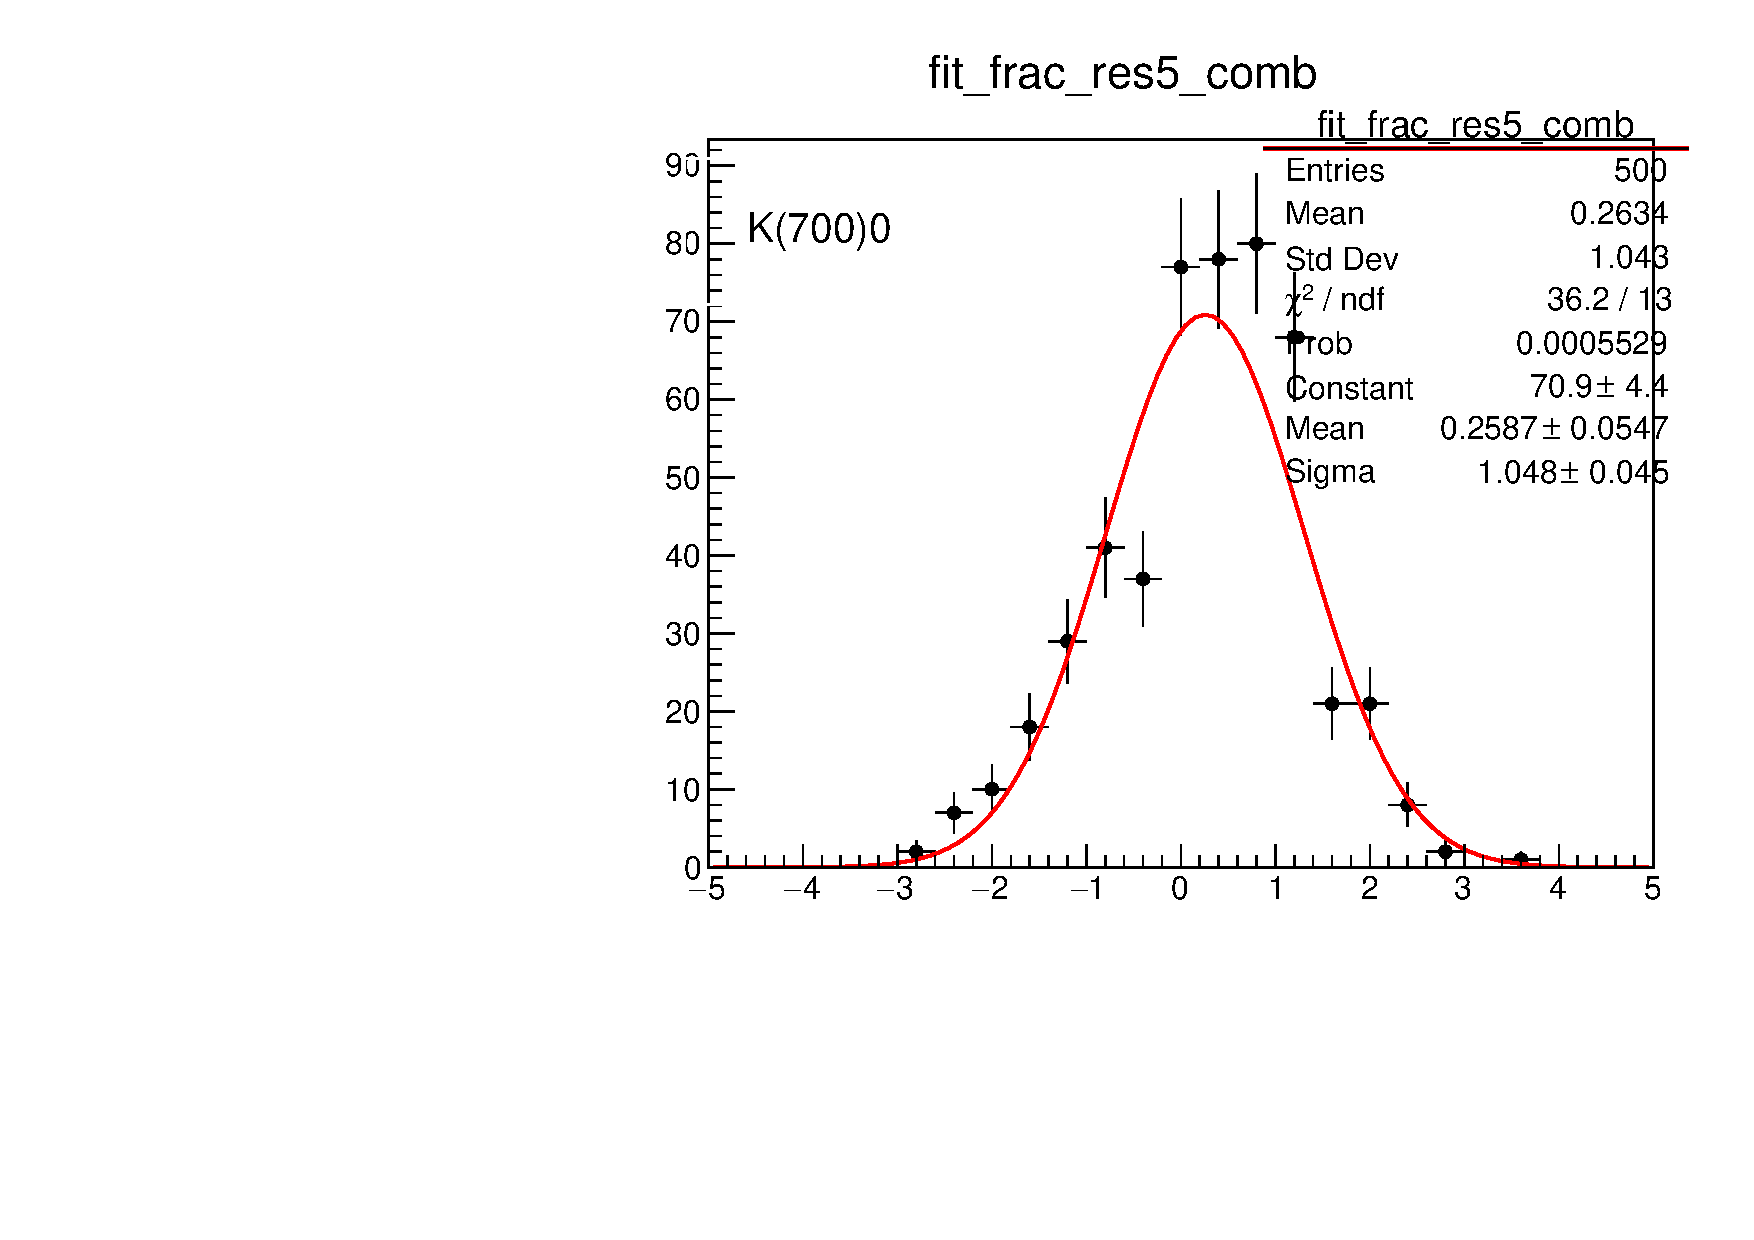
\includegraphics[width=0.24\textwidth]{figure/io_wo_bkg/fitfrac/pull_fitfrac_res5_comb.pdf}
    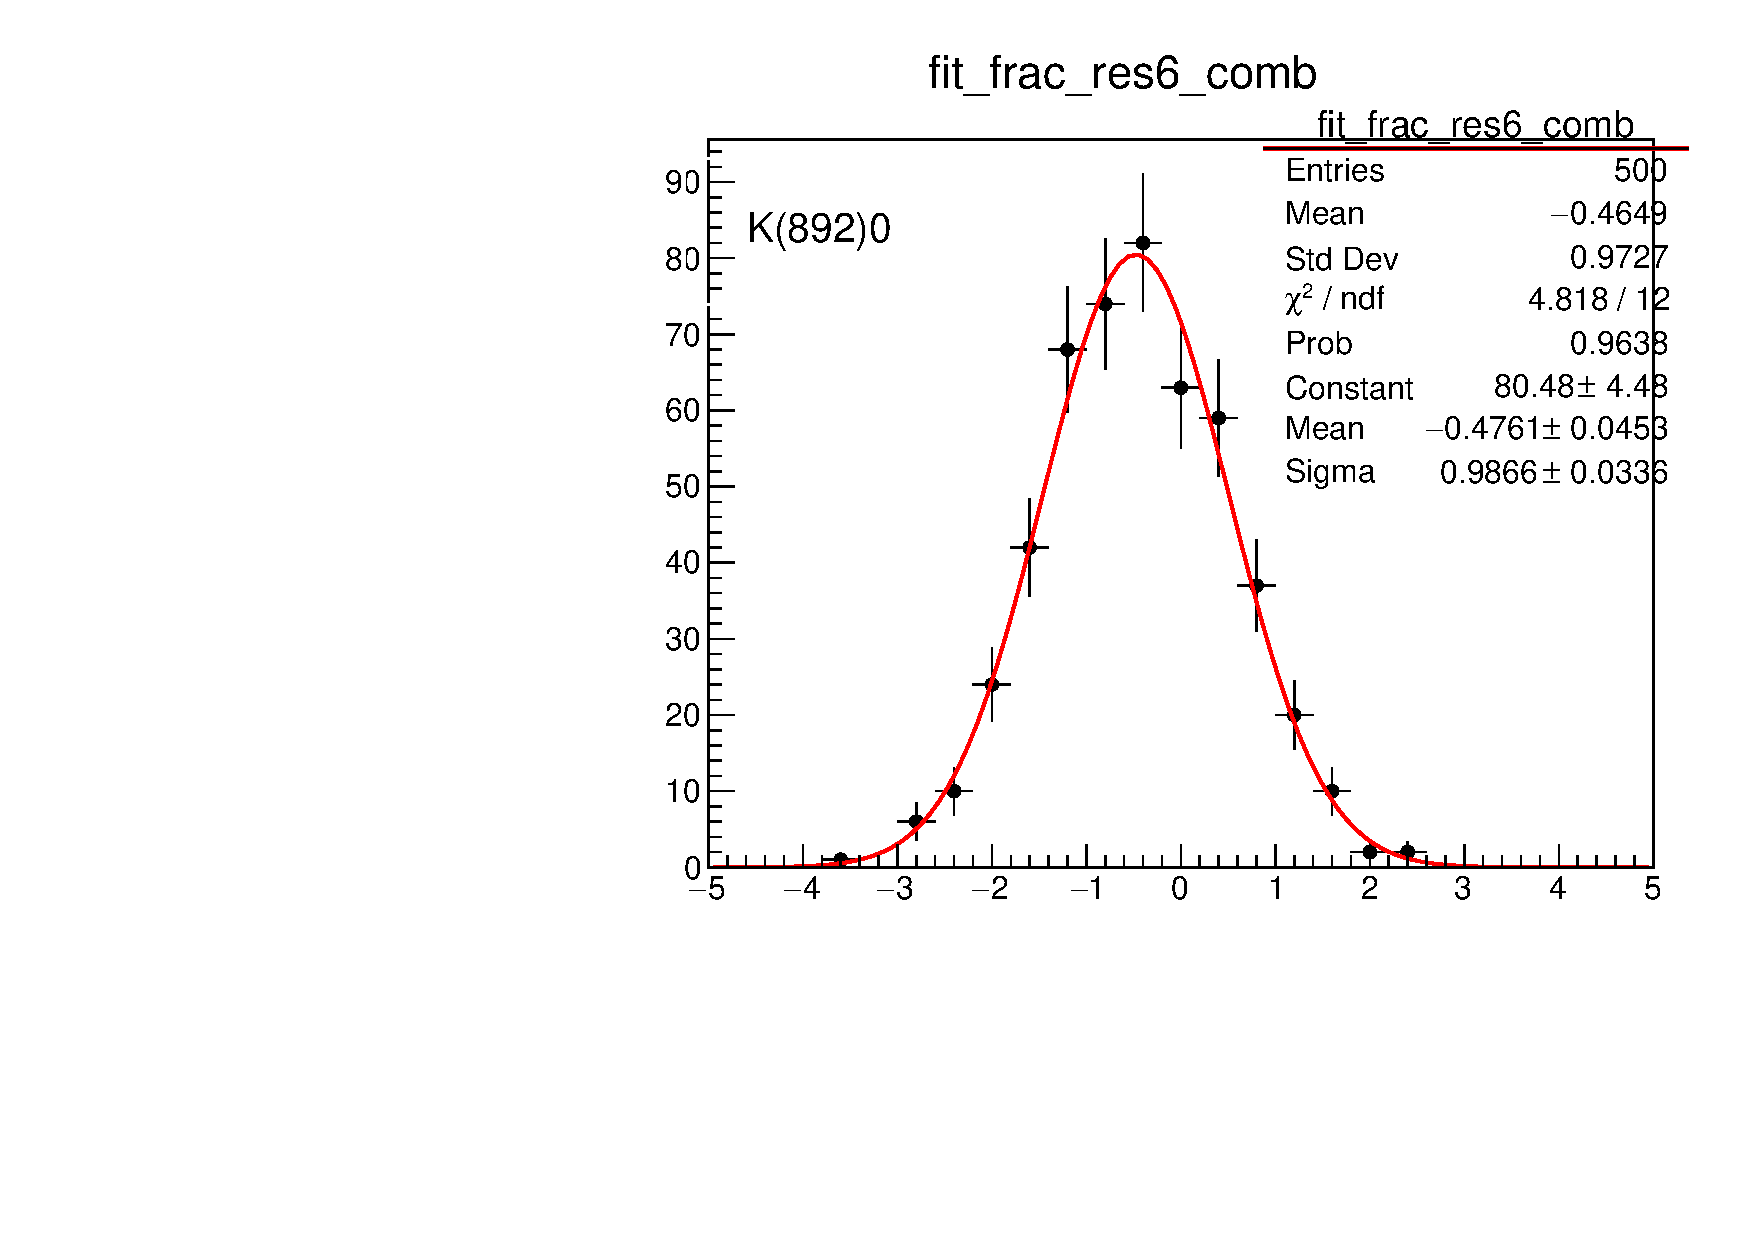
\includegraphics[width=0.24\textwidth]{figure/io_wo_bkg/fitfrac/pull_fitfrac_res6_comb.pdf}
    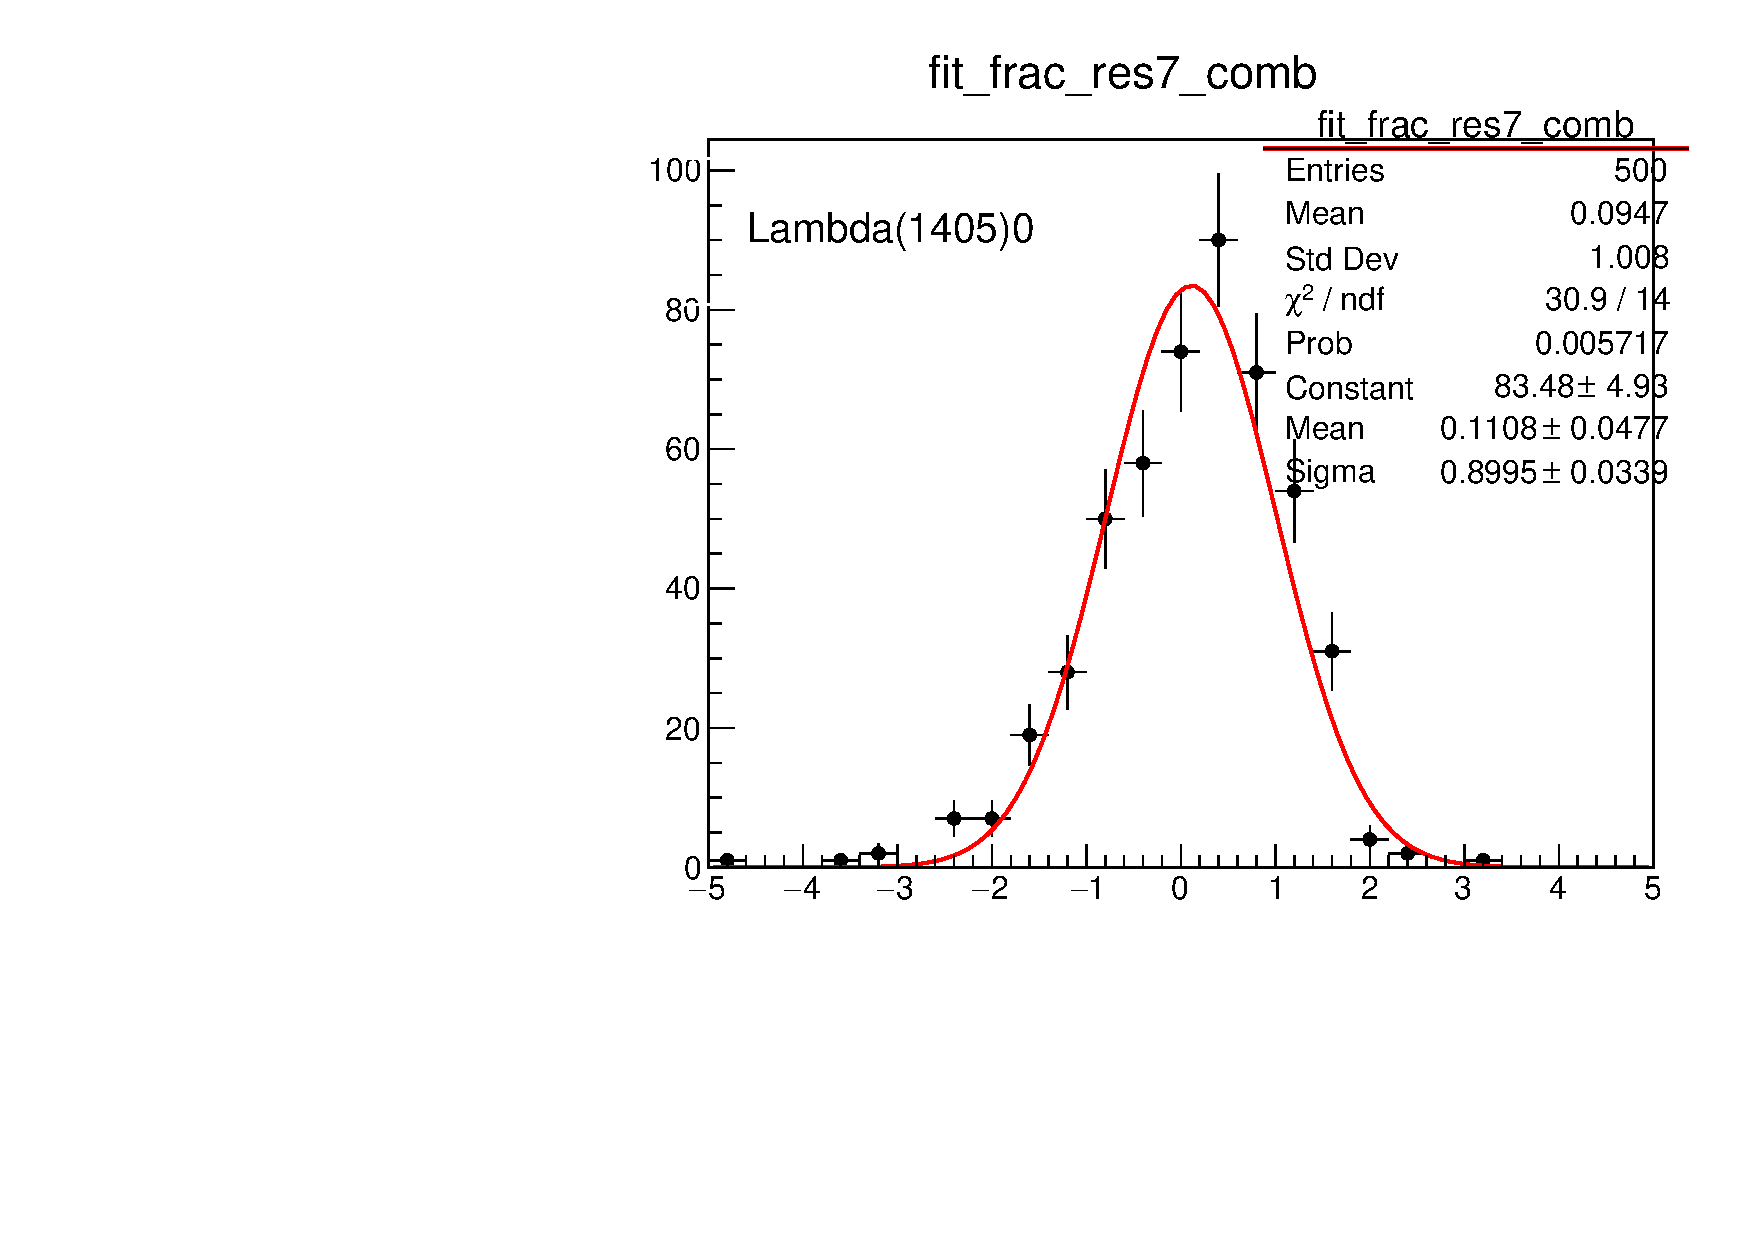
\includegraphics[width=0.24\textwidth]{figure/io_wo_bkg/fitfrac/pull_fitfrac_res7_comb.pdf}
    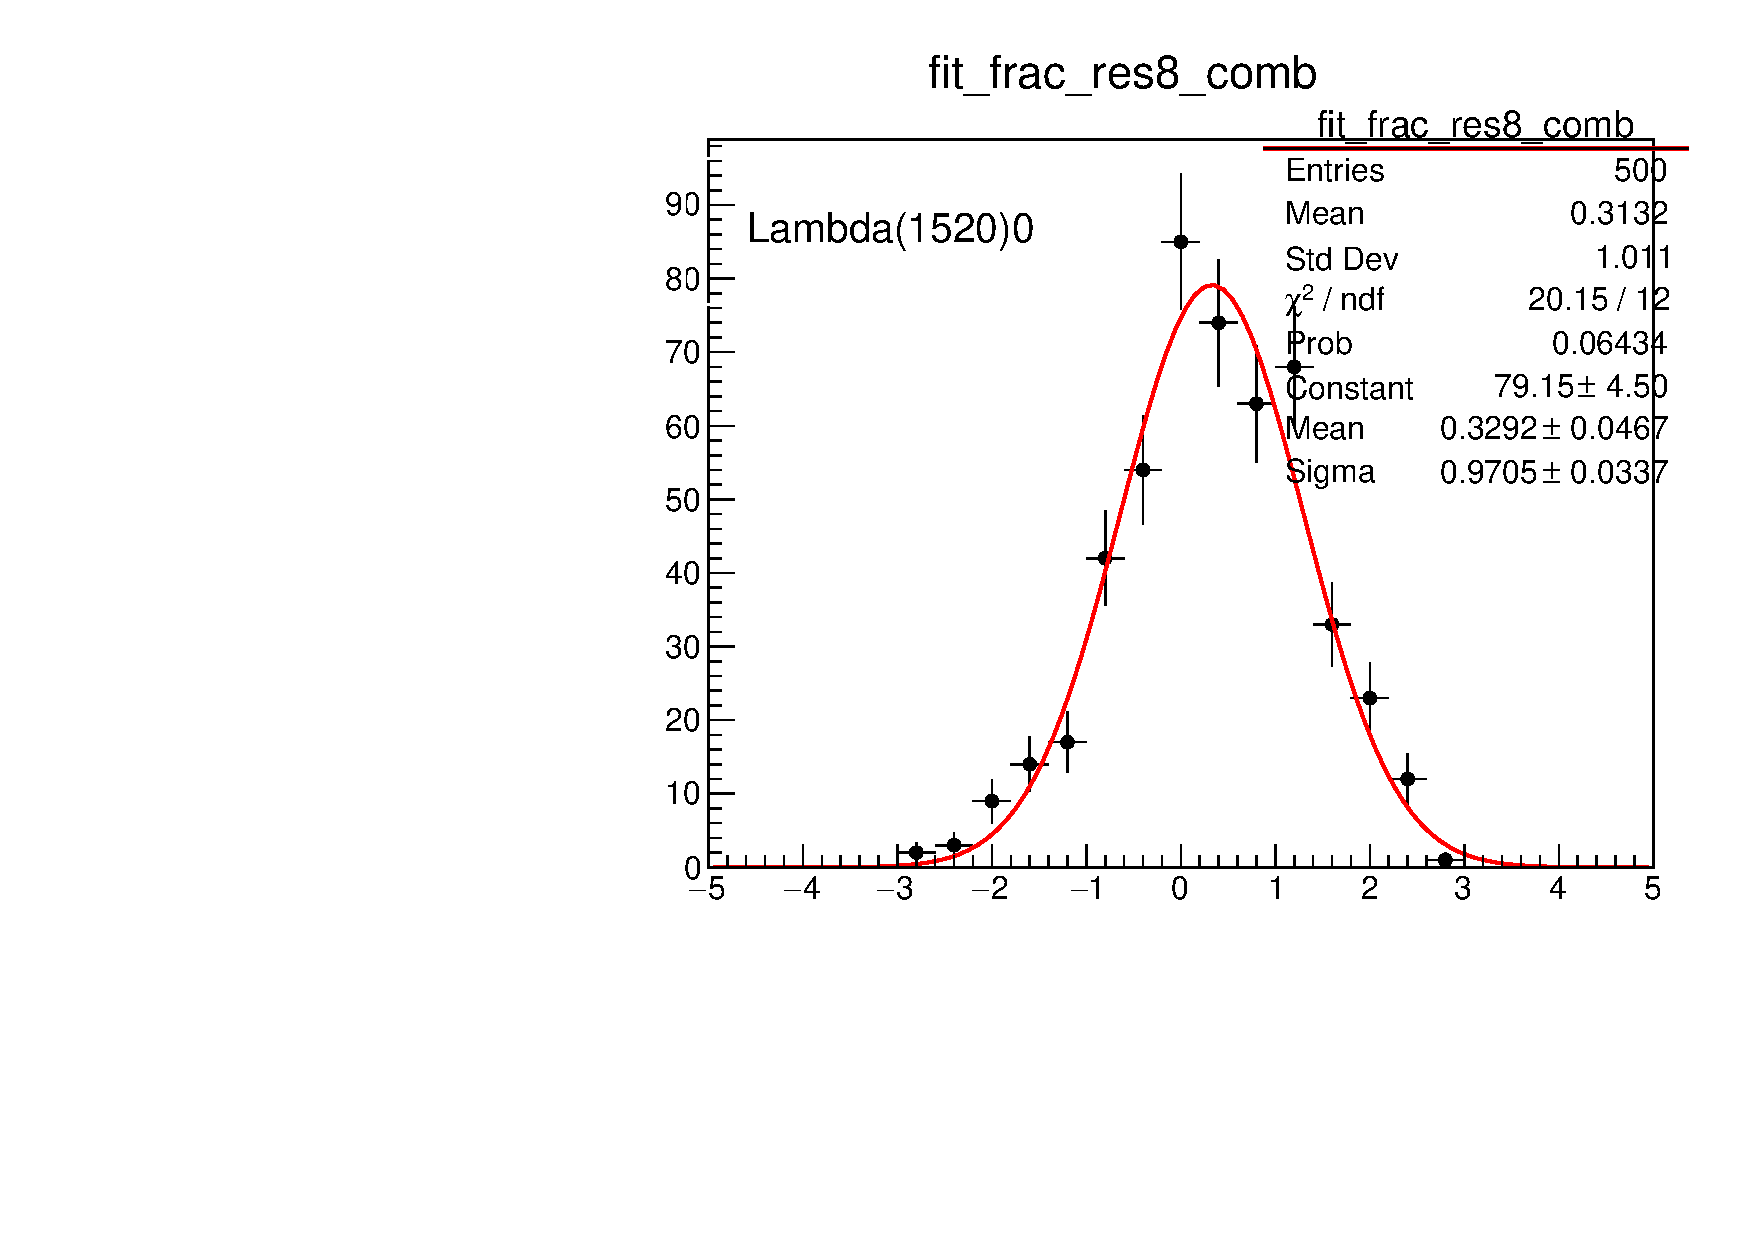
\includegraphics[width=0.24\textwidth]{figure/io_wo_bkg/fitfrac/pull_fitfrac_res8_comb.pdf}
    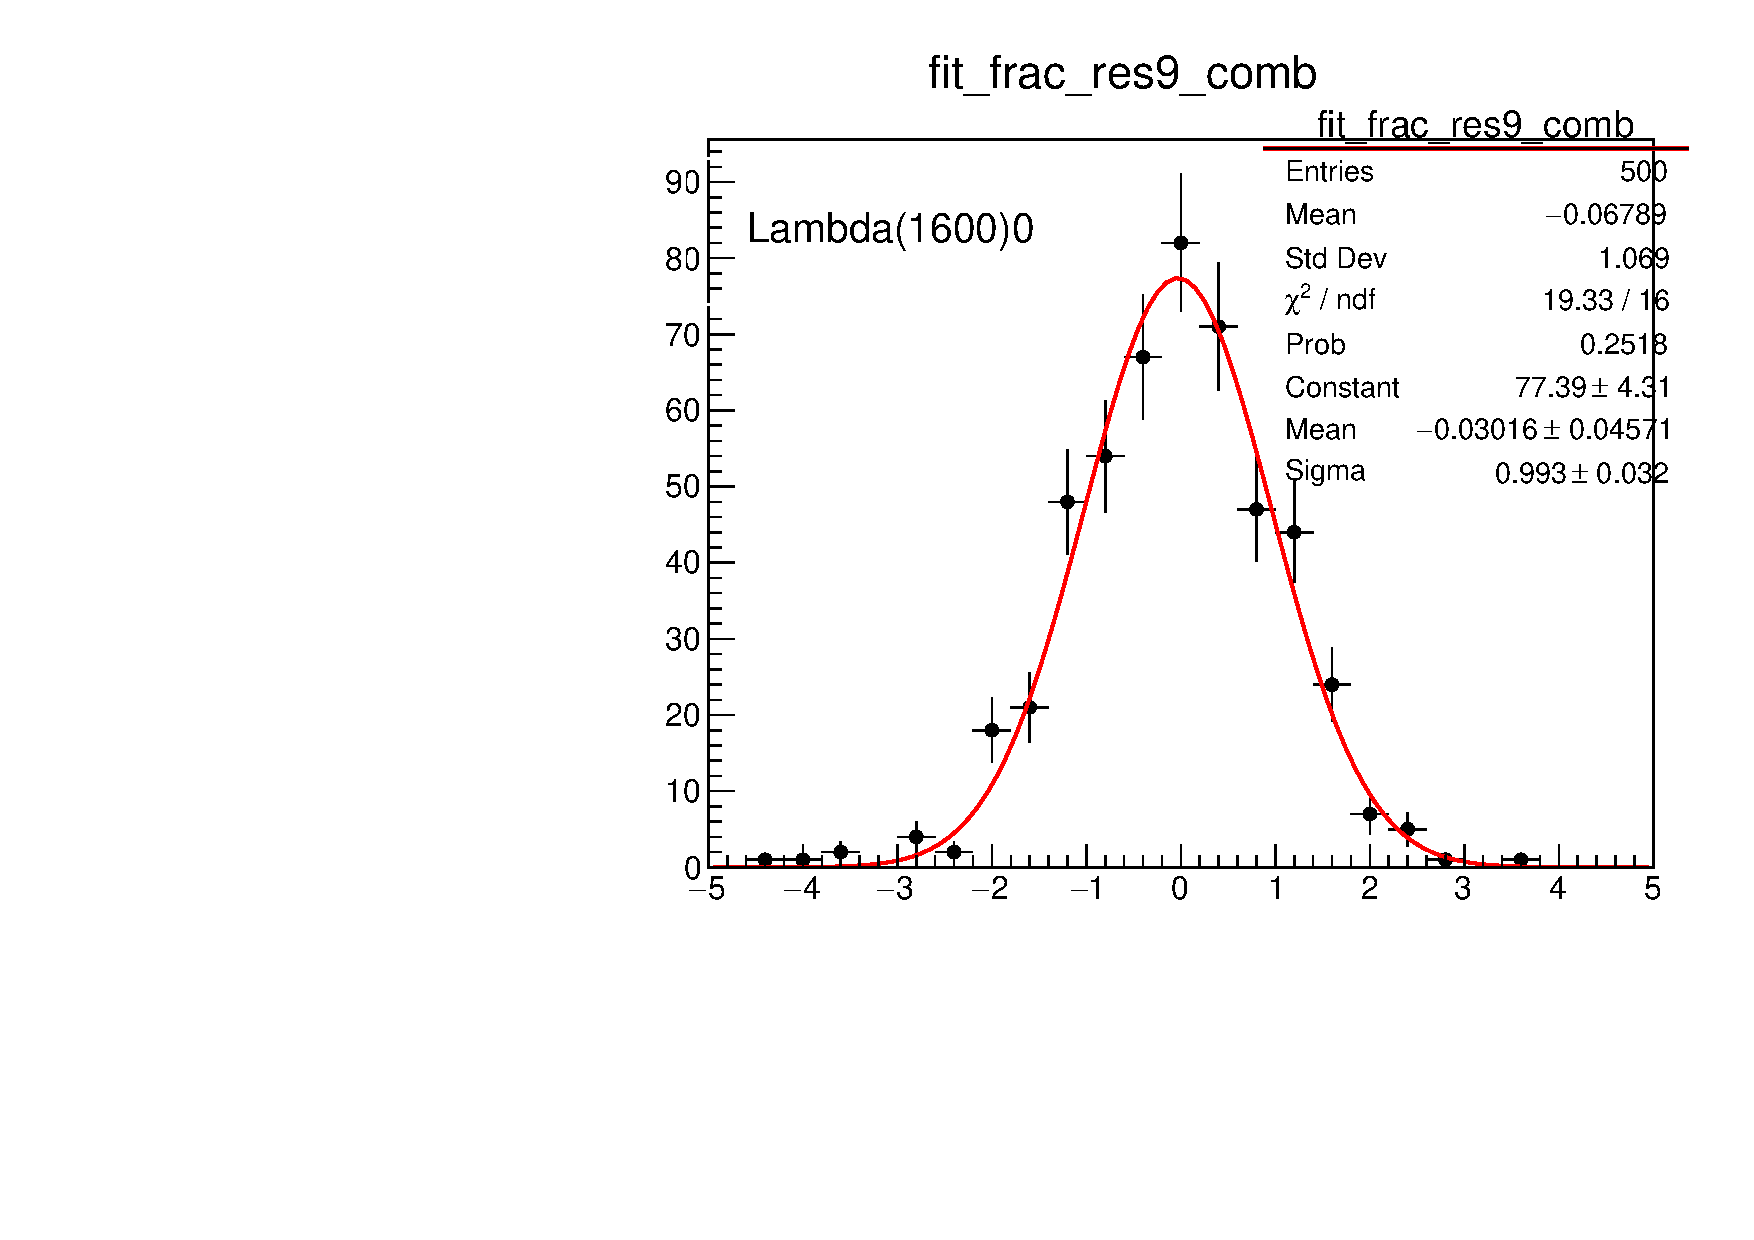
\includegraphics[width=0.24\textwidth]{figure/io_wo_bkg/fitfrac/pull_fitfrac_res9_comb.pdf}
    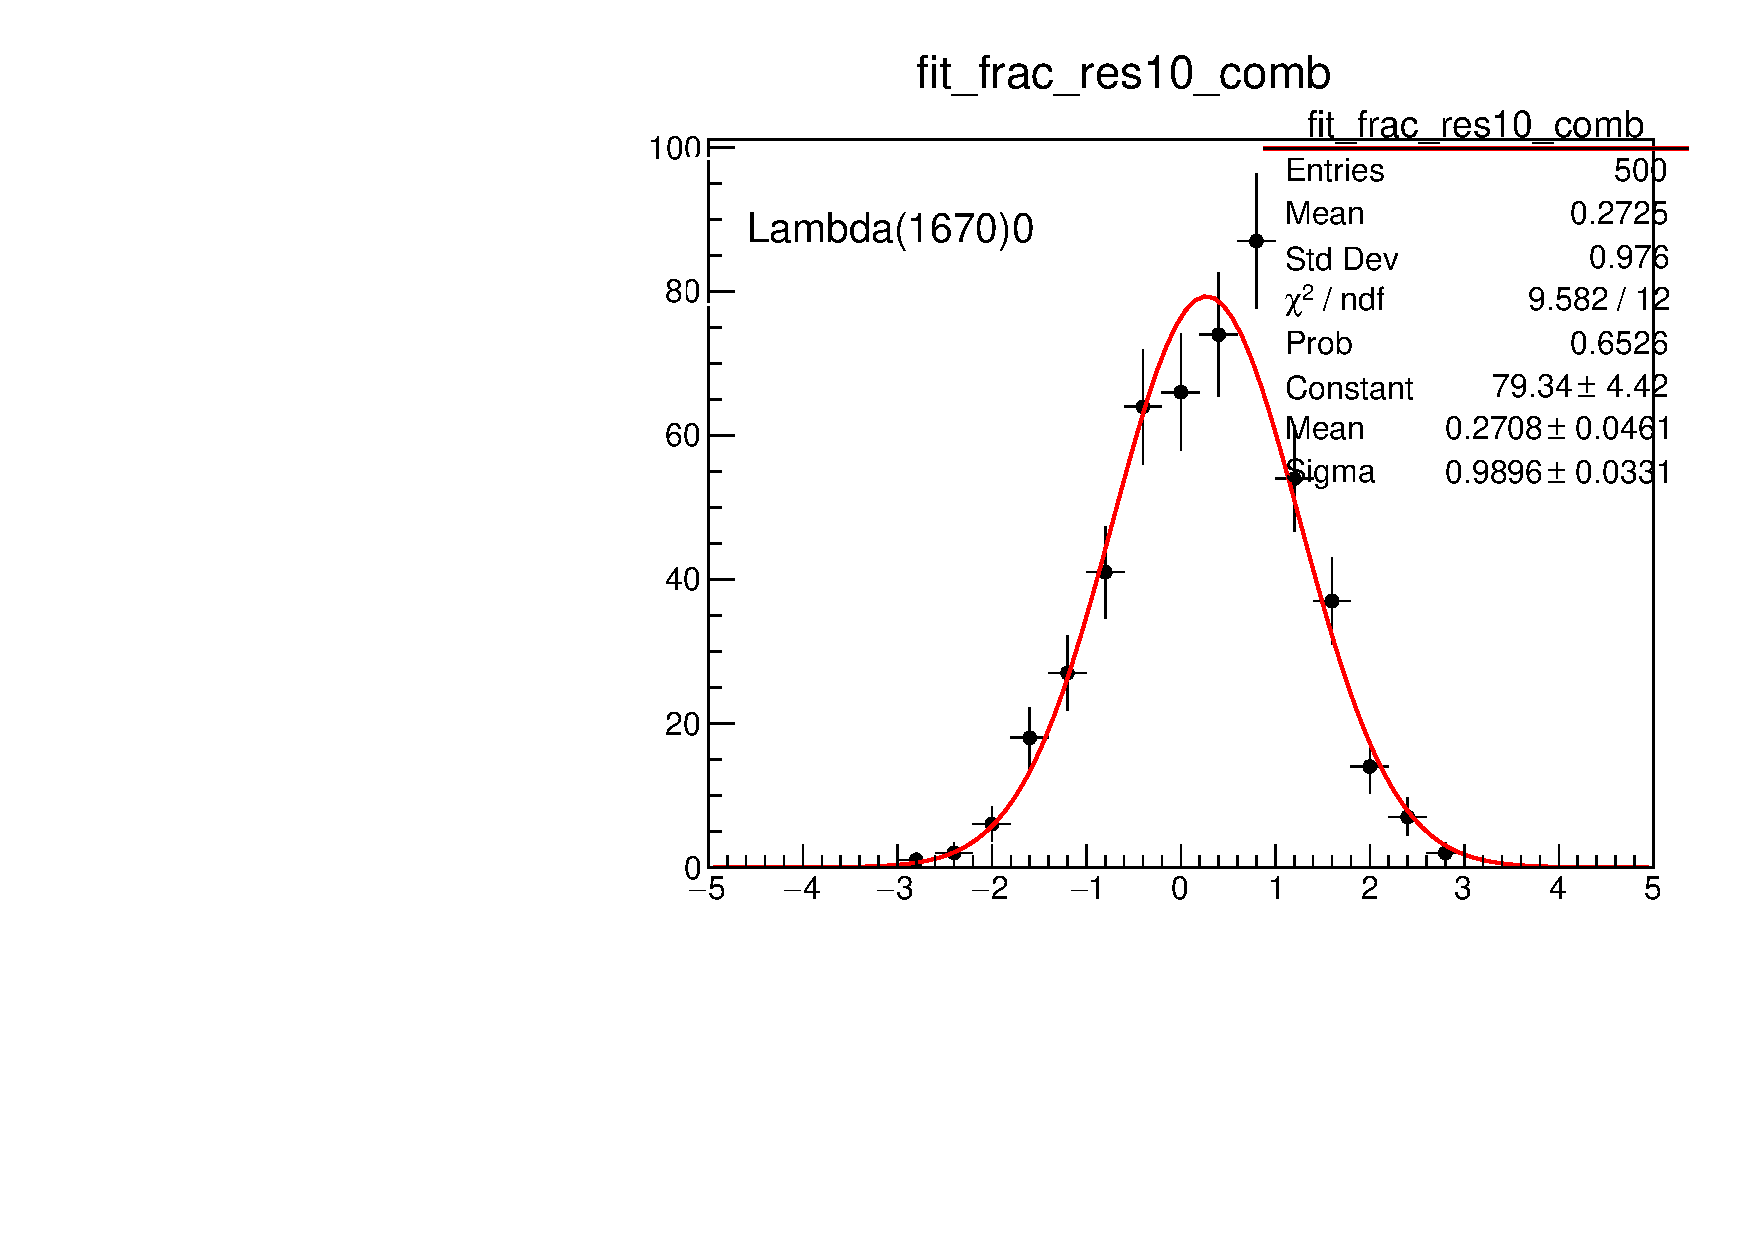
\includegraphics[width=0.24\textwidth]{figure/io_wo_bkg/fitfrac/pull_fitfrac_res10_comb.pdf}
    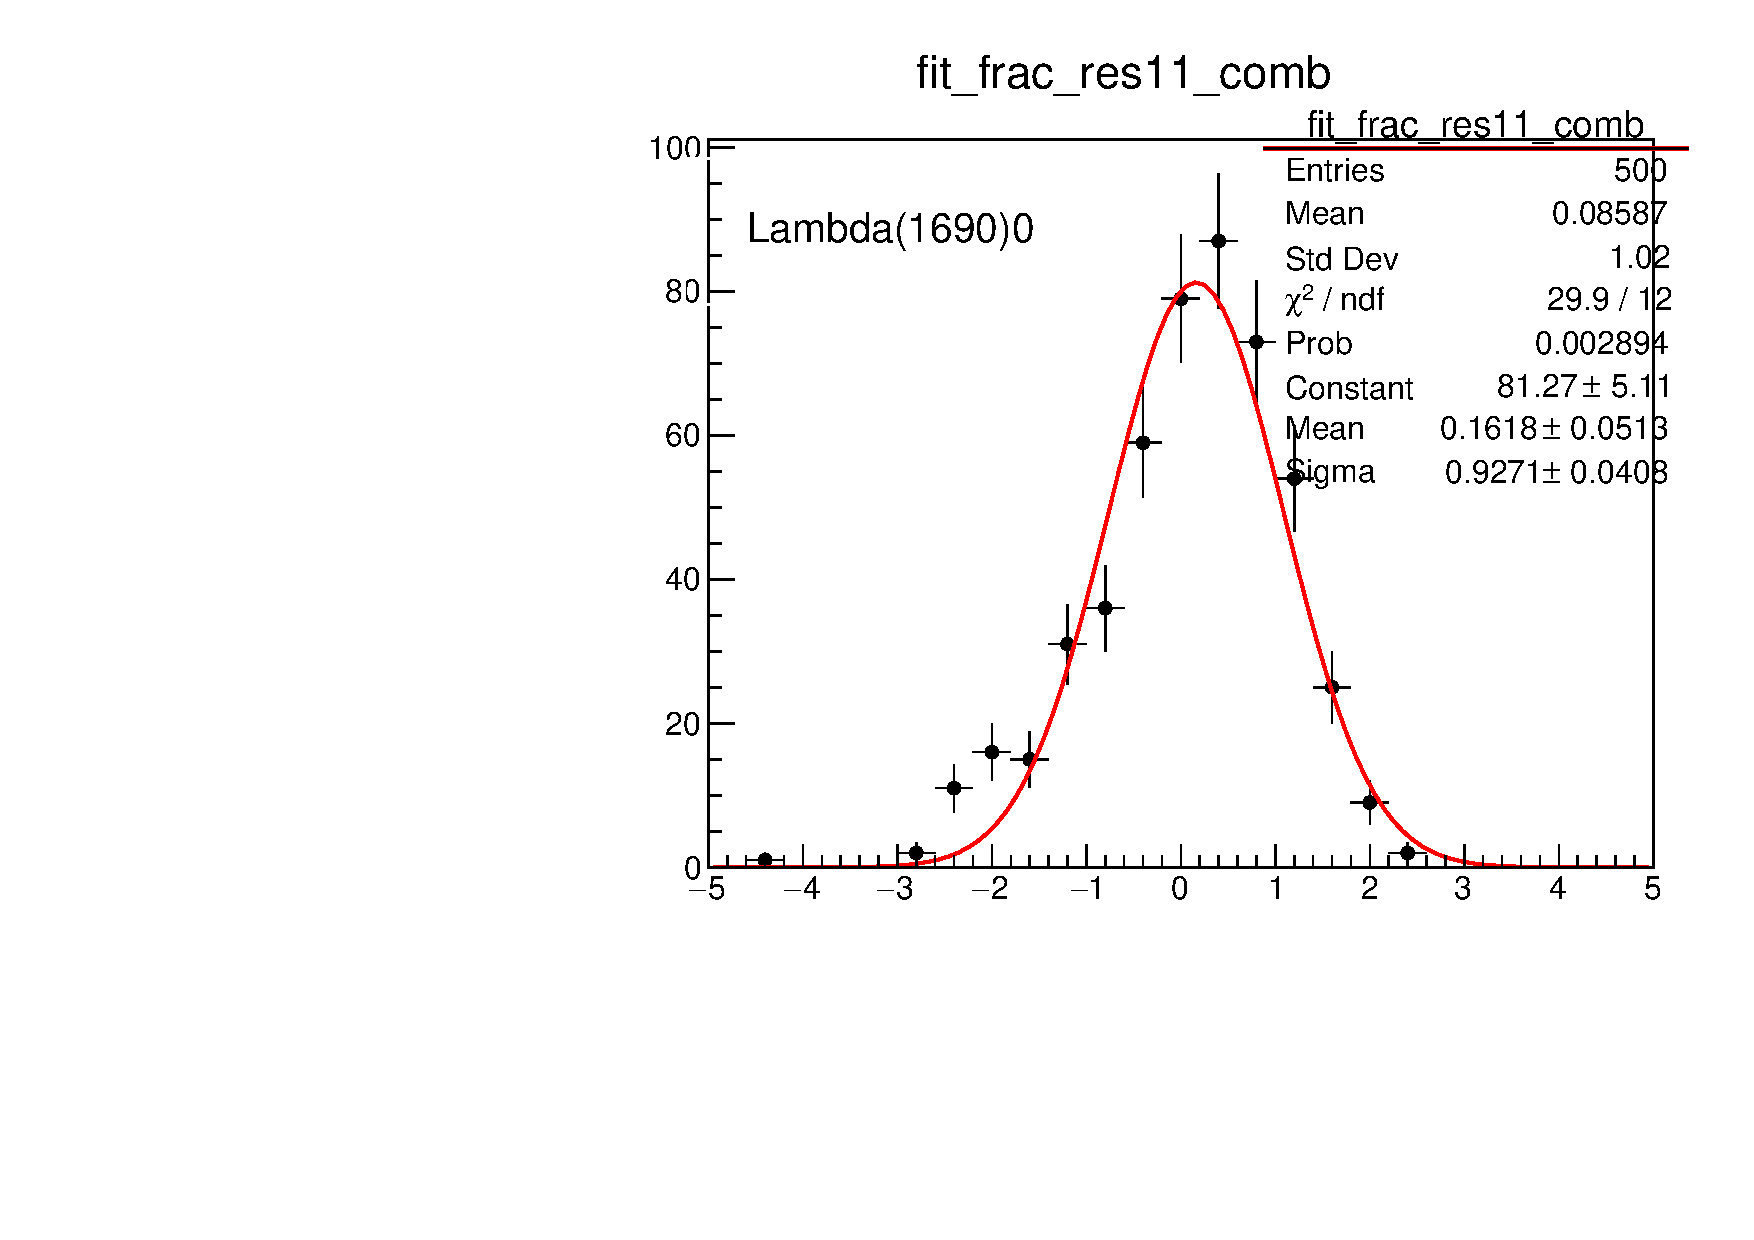
\includegraphics[width=0.24\textwidth]{figure/io_wo_bkg/fitfrac/pull_fitfrac_res11_comb.pdf}
    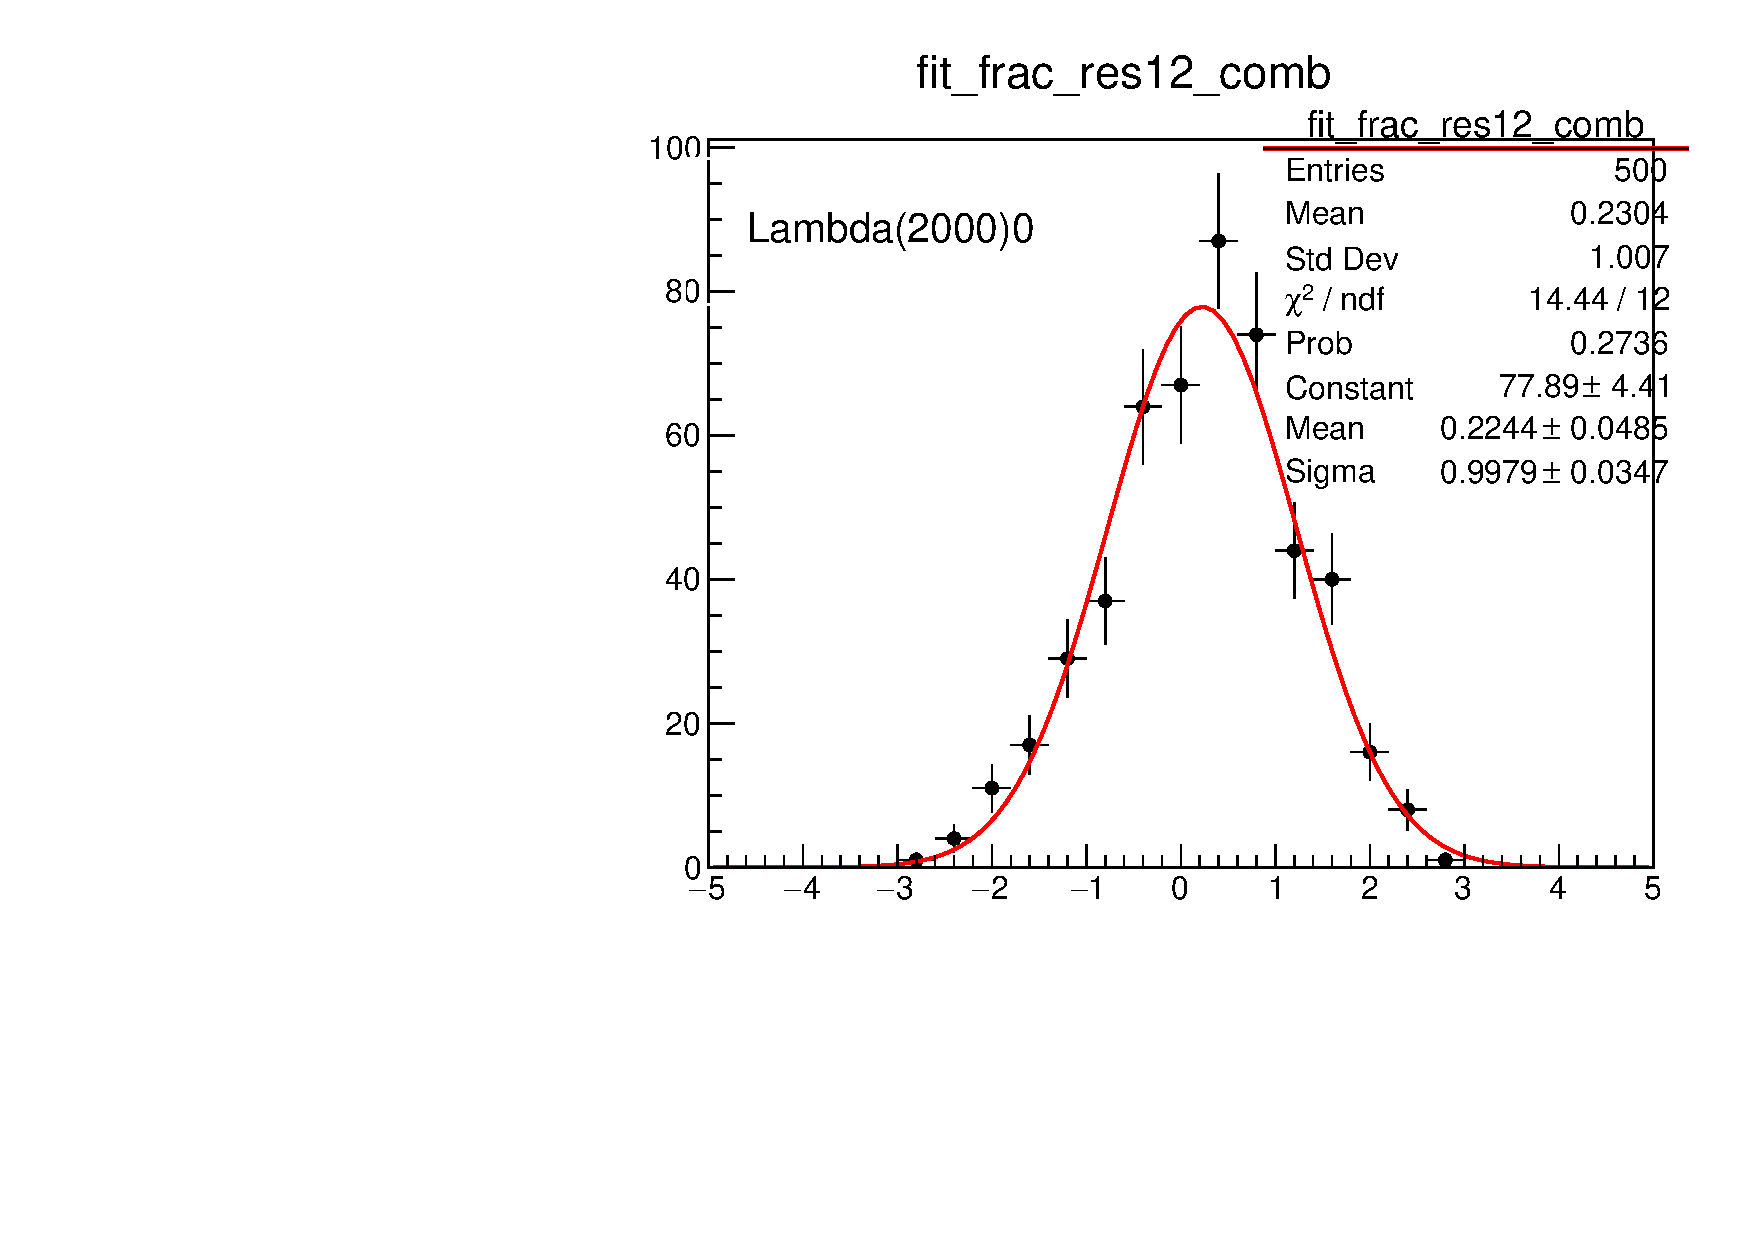
\includegraphics[width=0.24\textwidth]{figure/io_wo_bkg/fitfrac/pull_fitfrac_res12_comb.pdf}
    \caption{Pull distributions of FF for each resonance.}
\label{fig:io_wo_bkg_pull_ff}
\end{figure}

\begin{figure}[h]\centering
    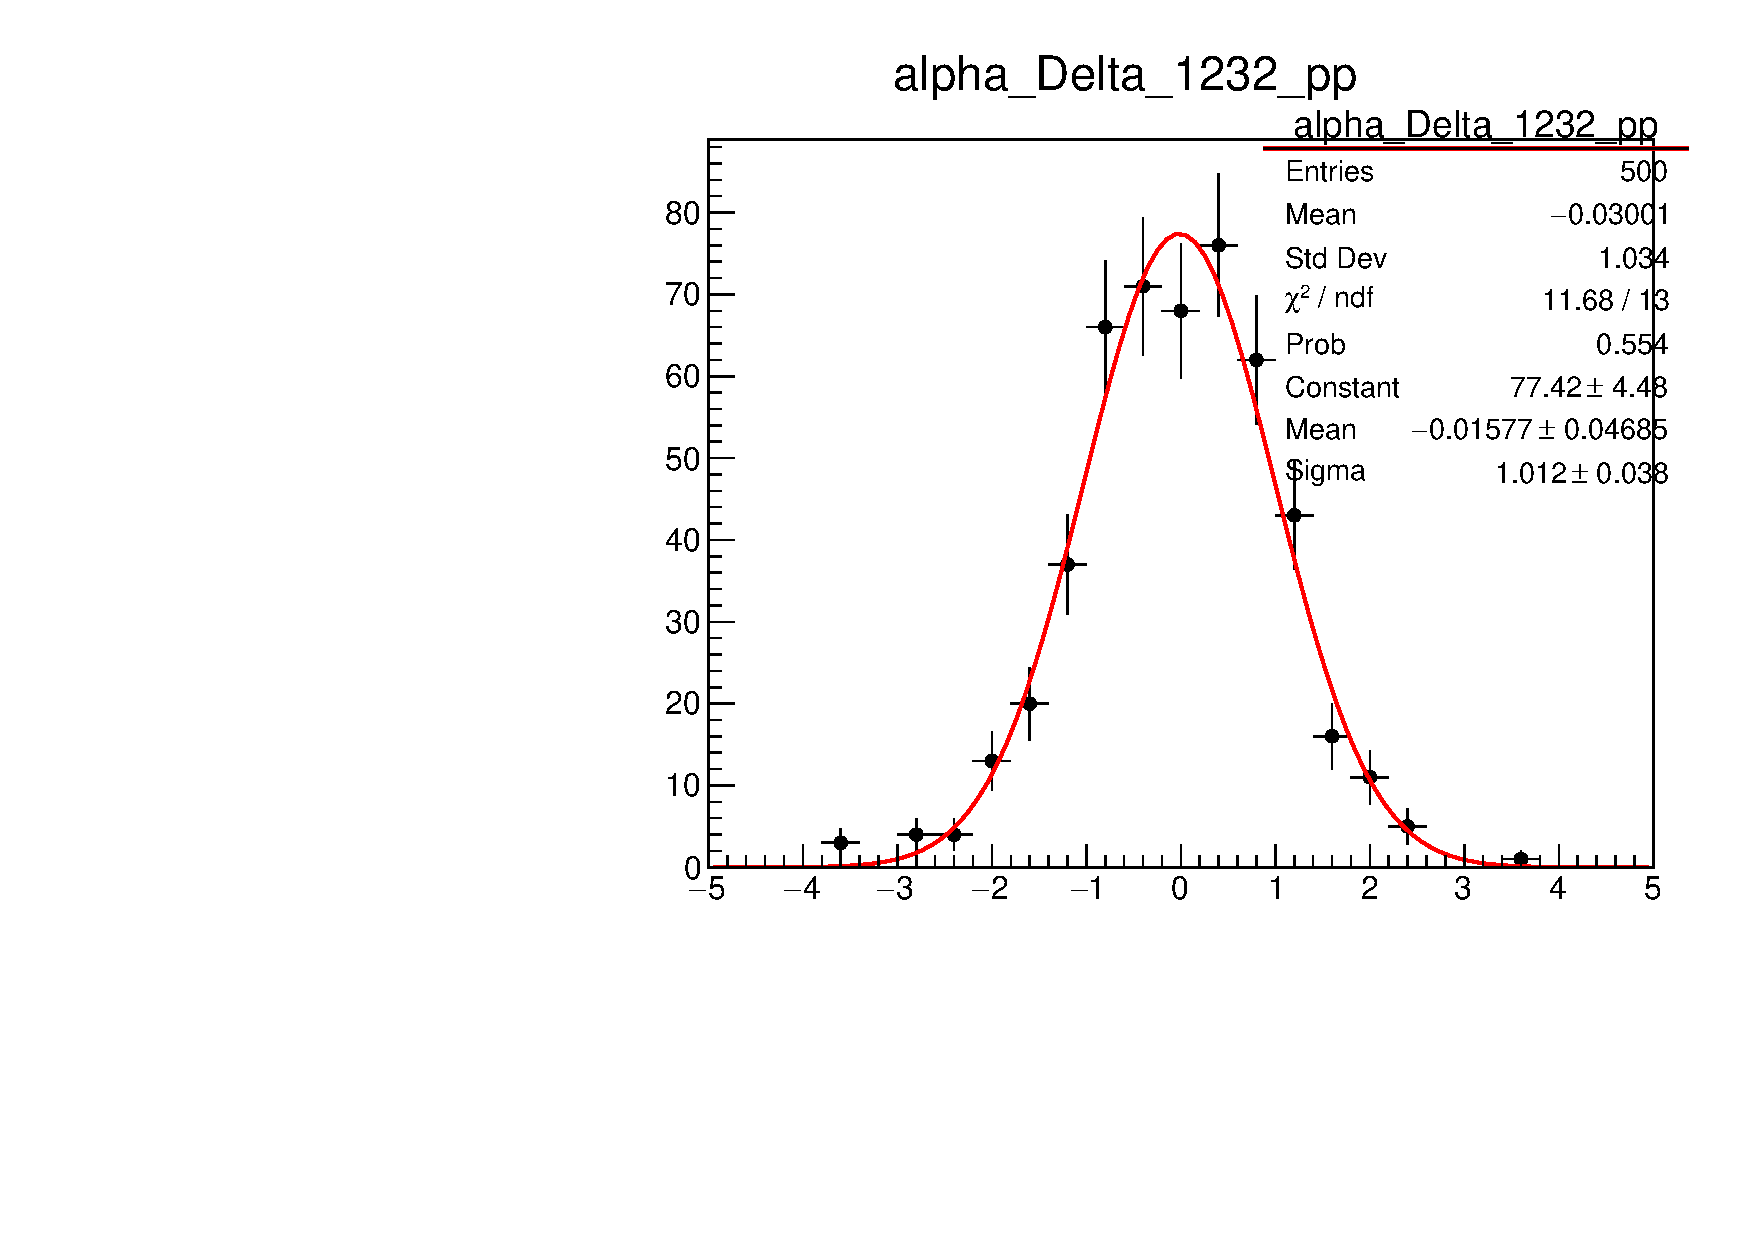
\includegraphics[width=0.24\textwidth]{figure/io_wo_bkg/alpha/pull_alpha_Delta_1232_pp.pdf}
    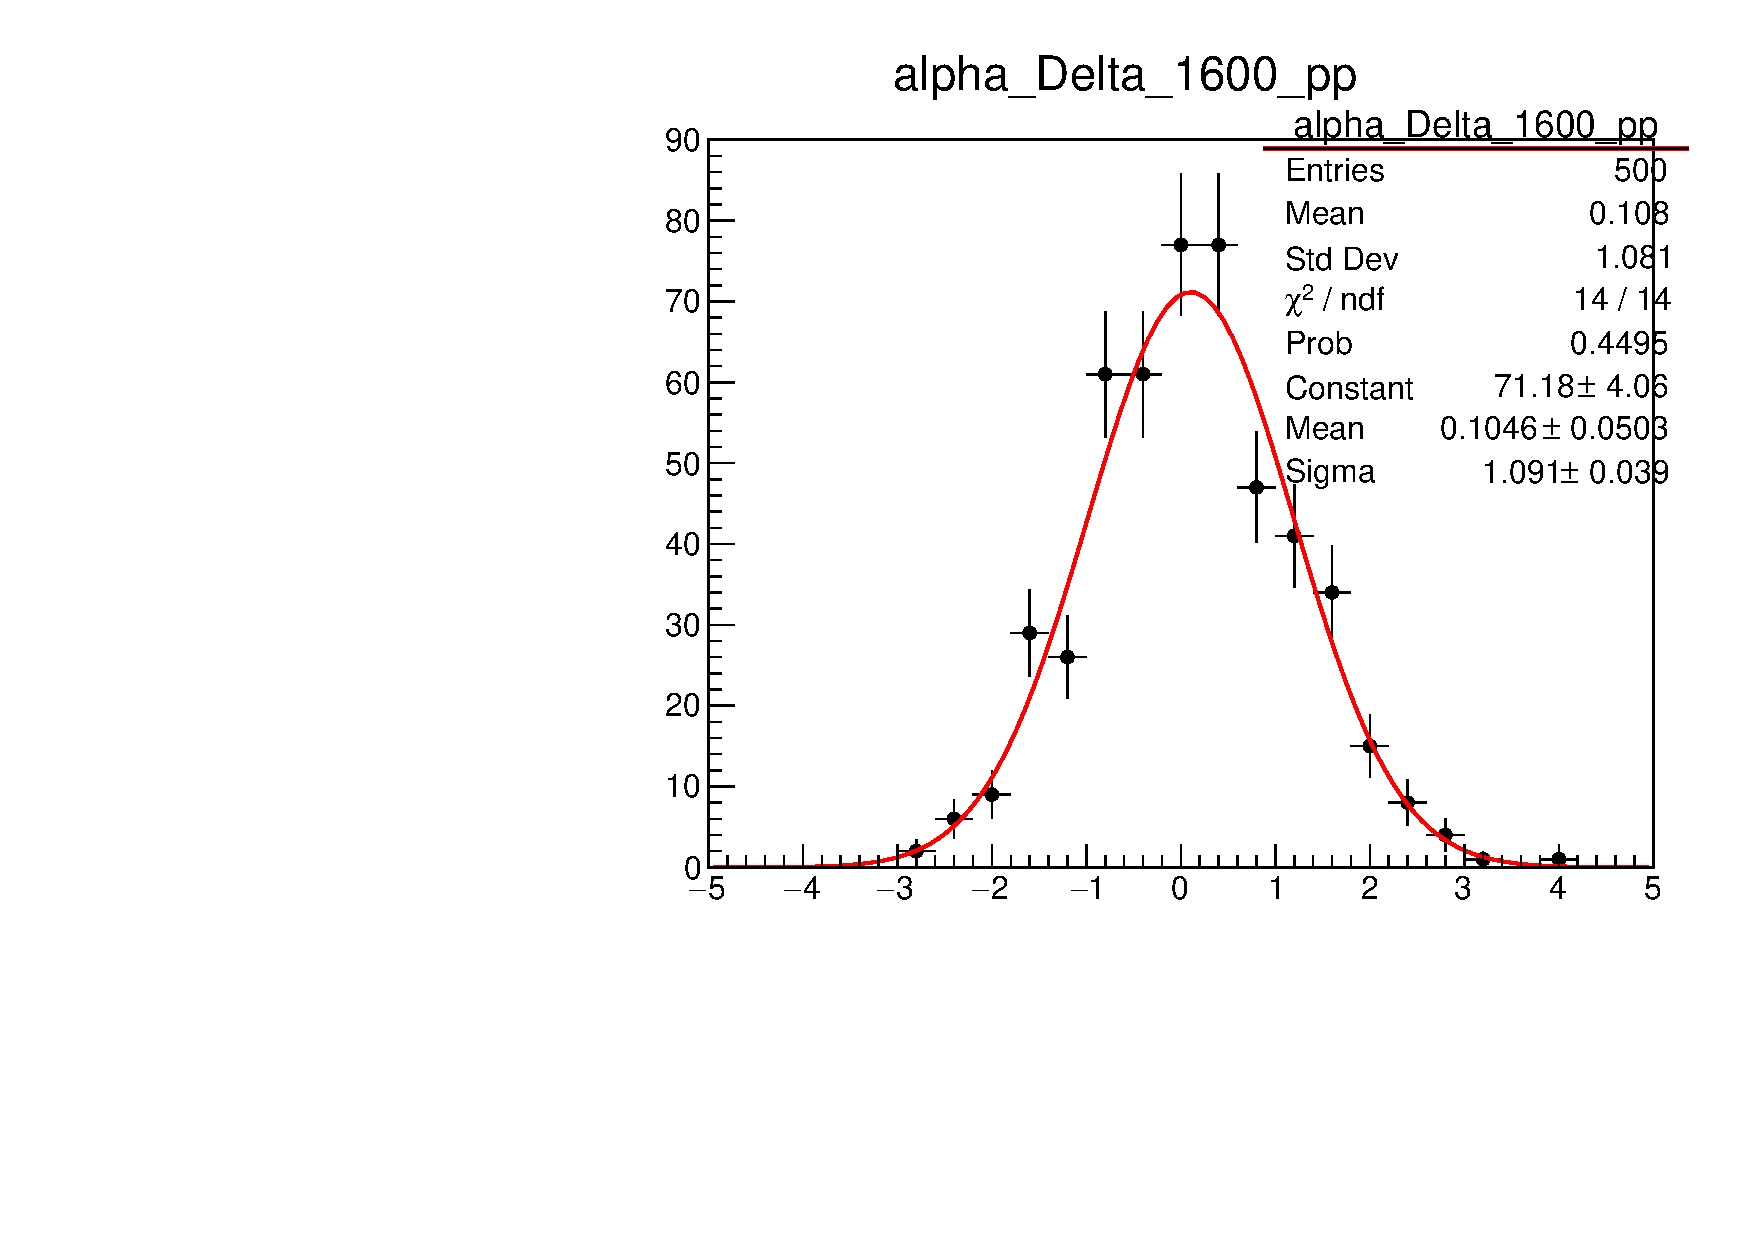
\includegraphics[width=0.24\textwidth]{figure/io_wo_bkg/alpha/pull_alpha_Delta_1600_pp.pdf}
    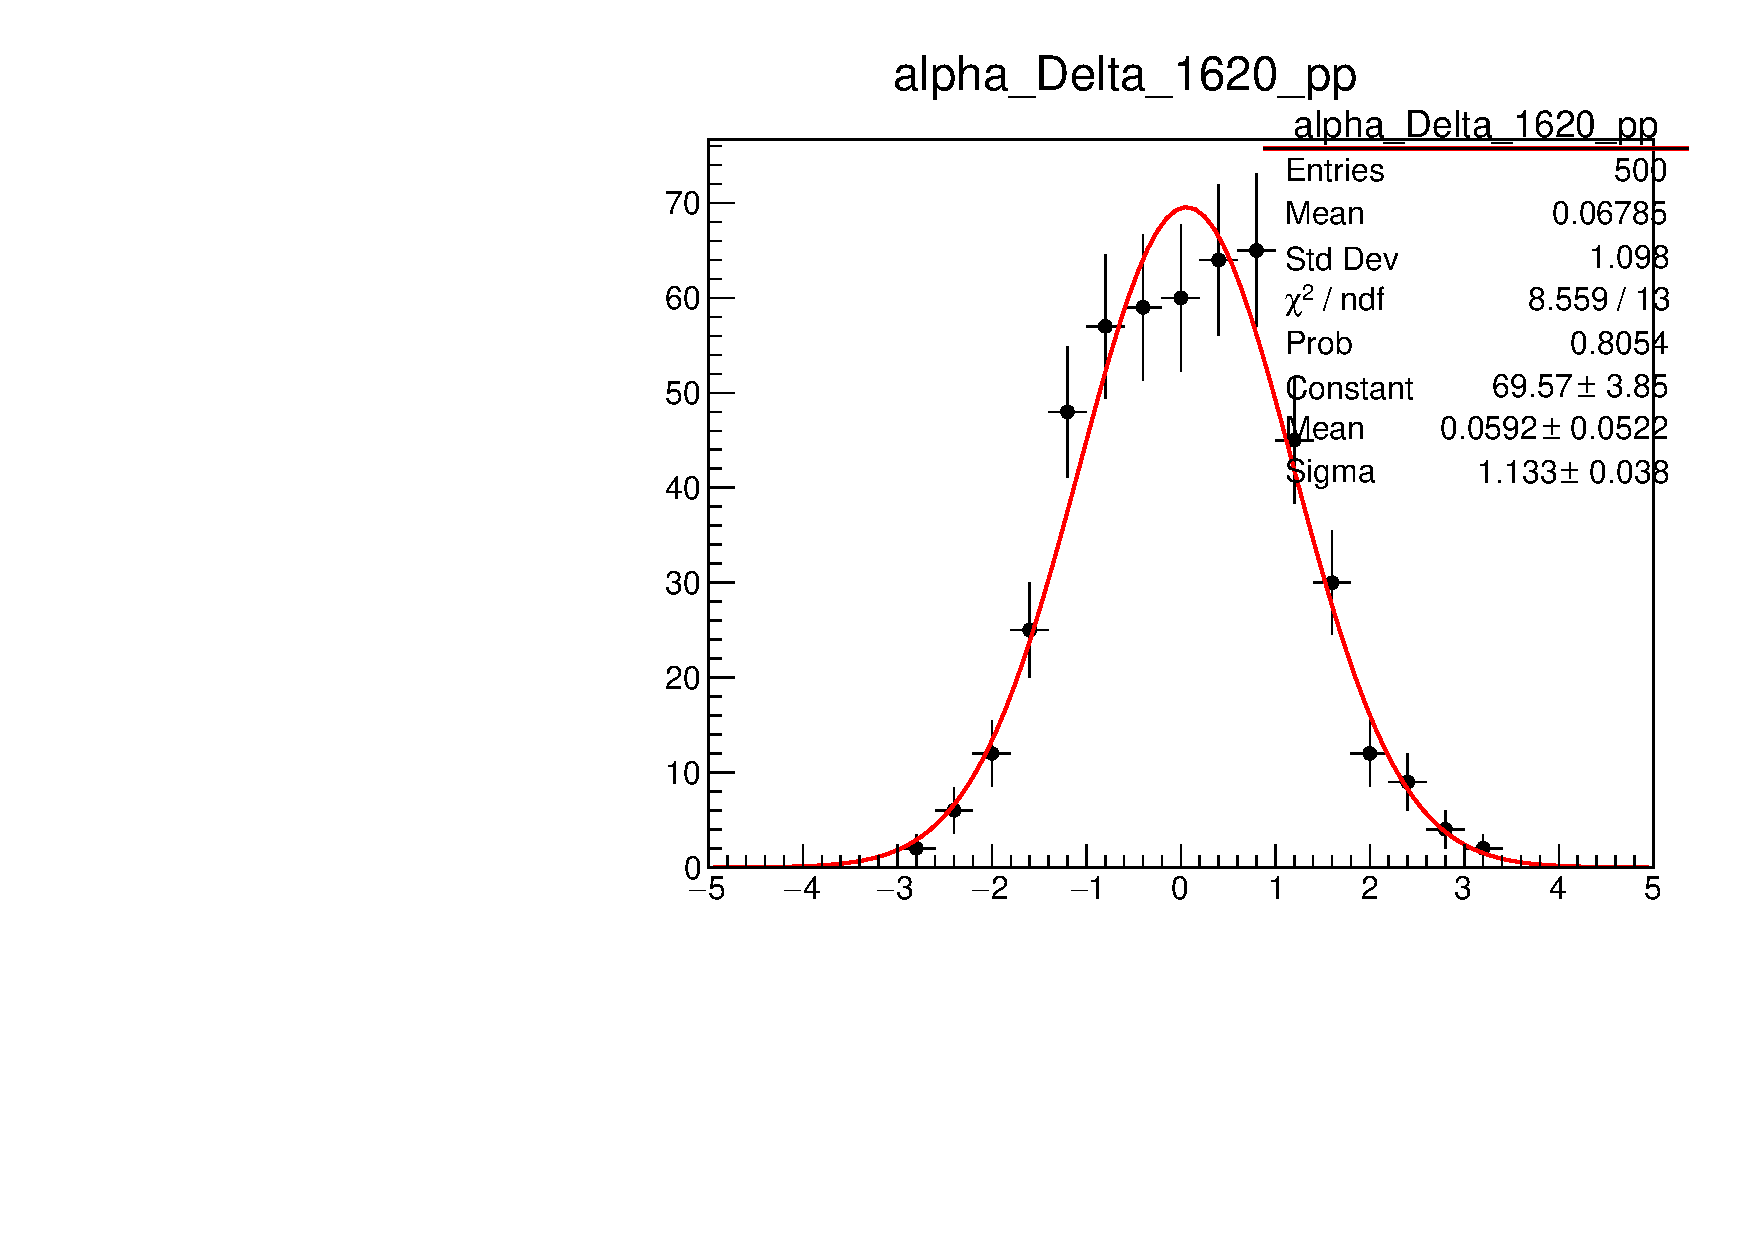
\includegraphics[width=0.24\textwidth]{figure/io_wo_bkg/alpha/pull_alpha_Delta_1620_pp.pdf}
    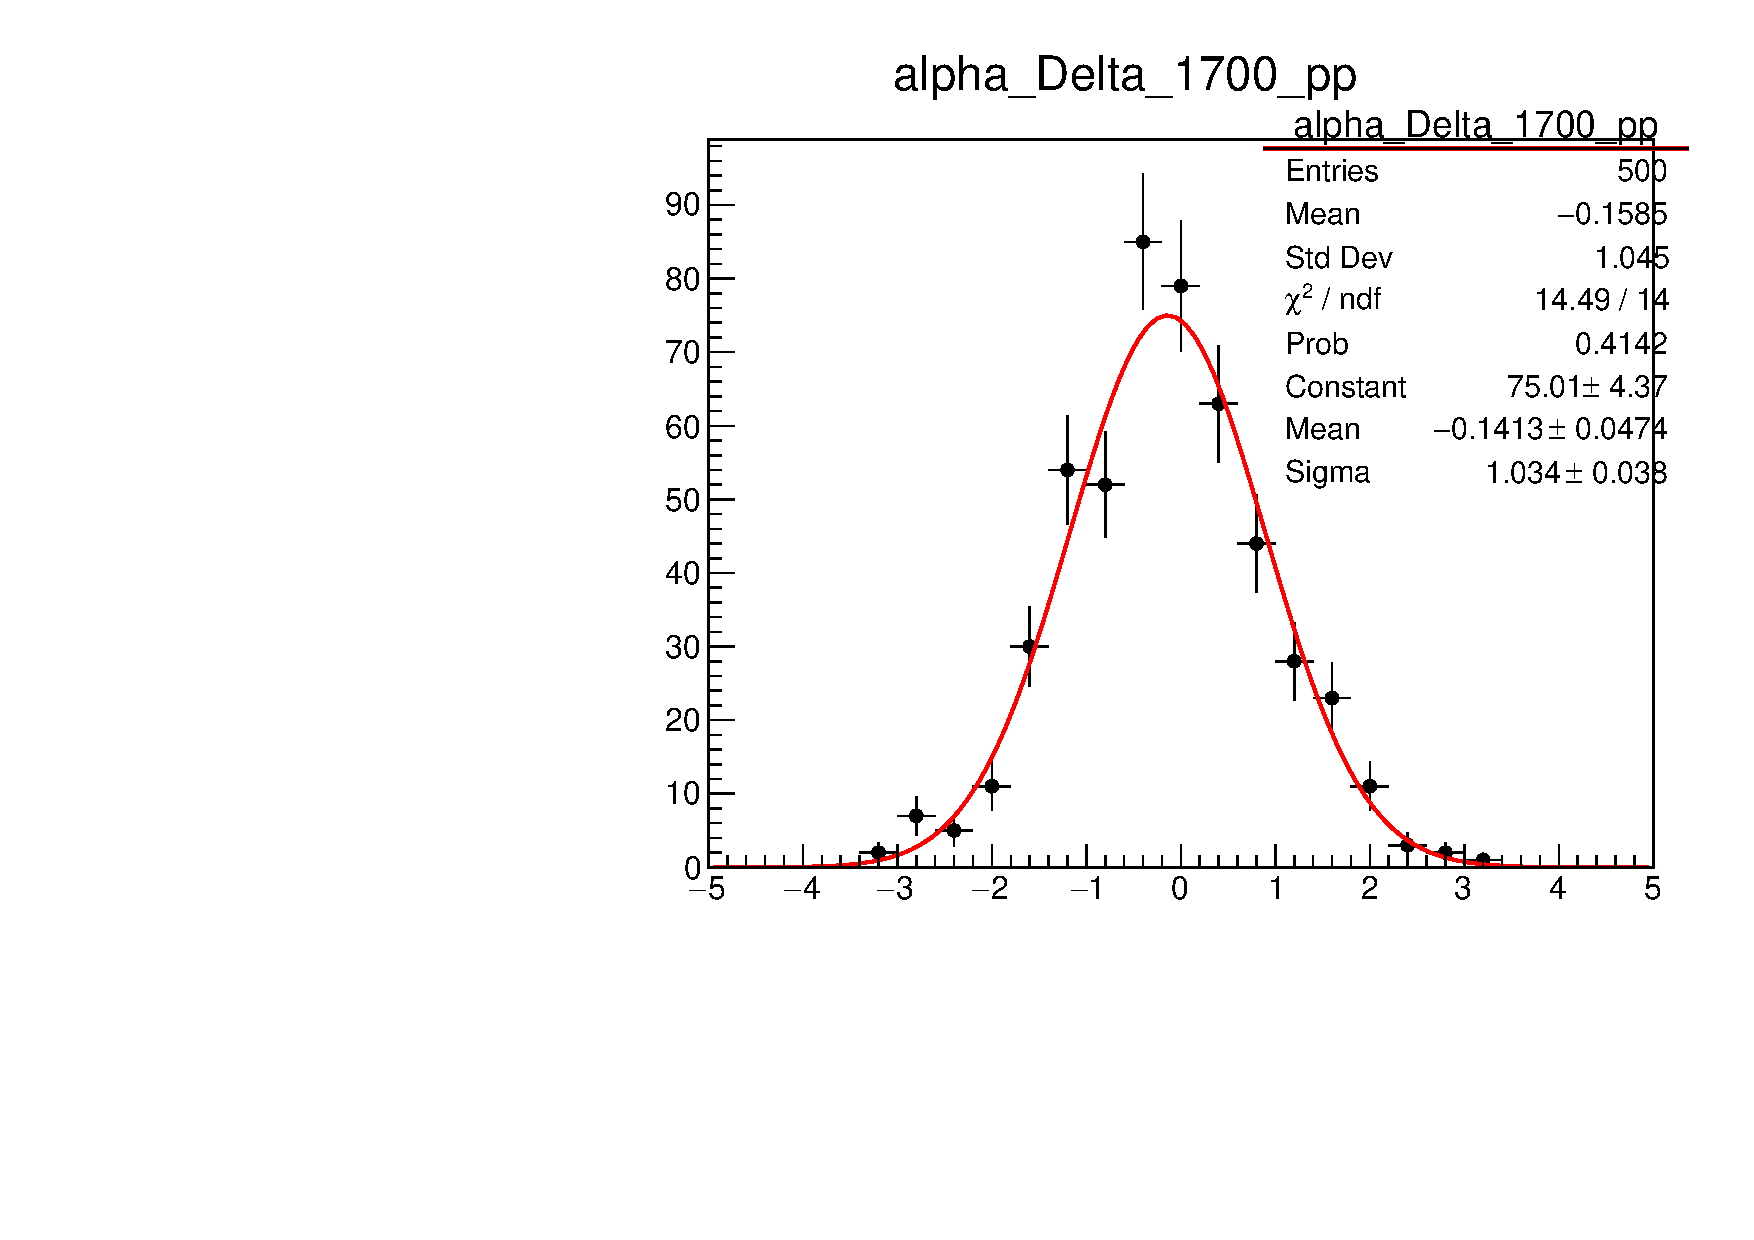
\includegraphics[width=0.24\textwidth]{figure/io_wo_bkg/alpha/pull_alpha_Delta_1700_pp.pdf}
    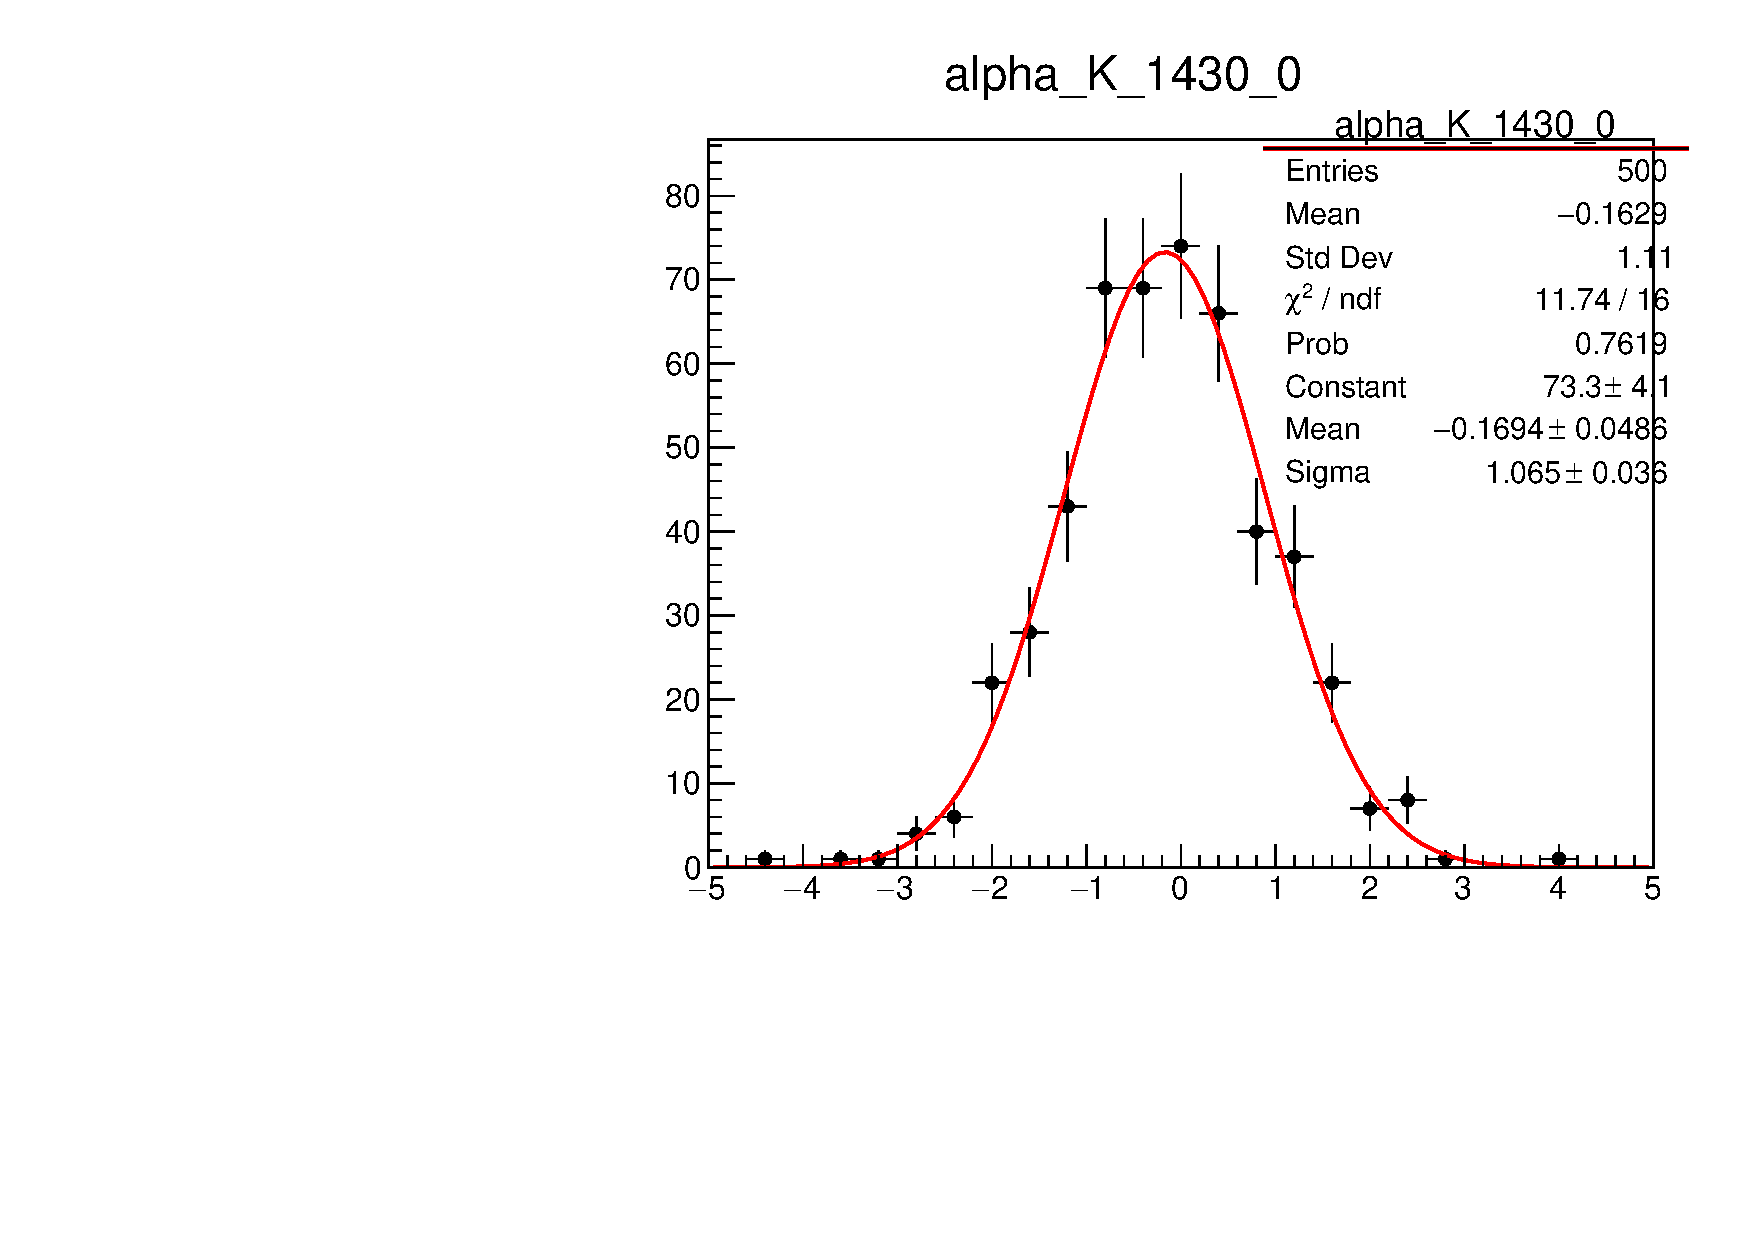
\includegraphics[width=0.24\textwidth]{figure/io_wo_bkg/alpha/pull_alpha_K_1430_0.pdf}
    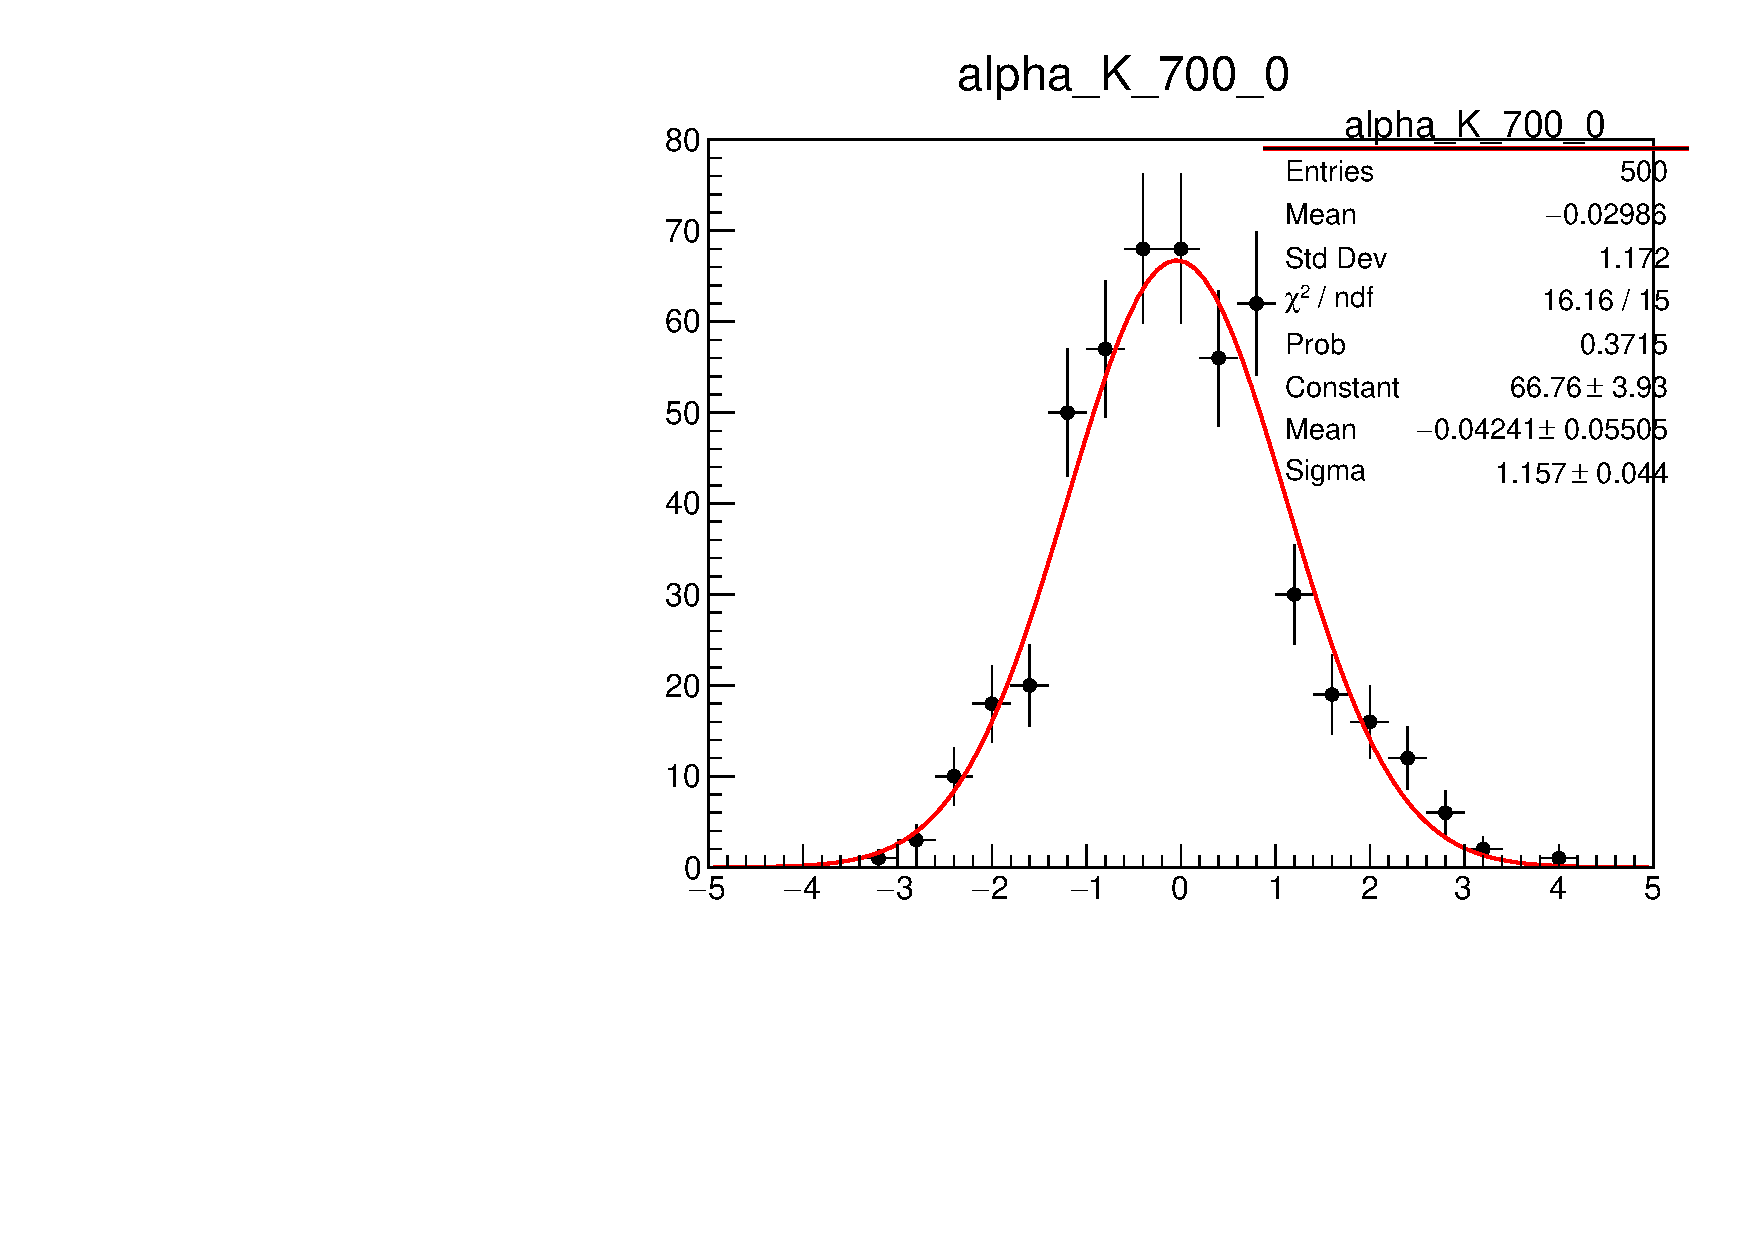
\includegraphics[width=0.24\textwidth]{figure/io_wo_bkg/alpha/pull_alpha_K_700_0.pdf}
    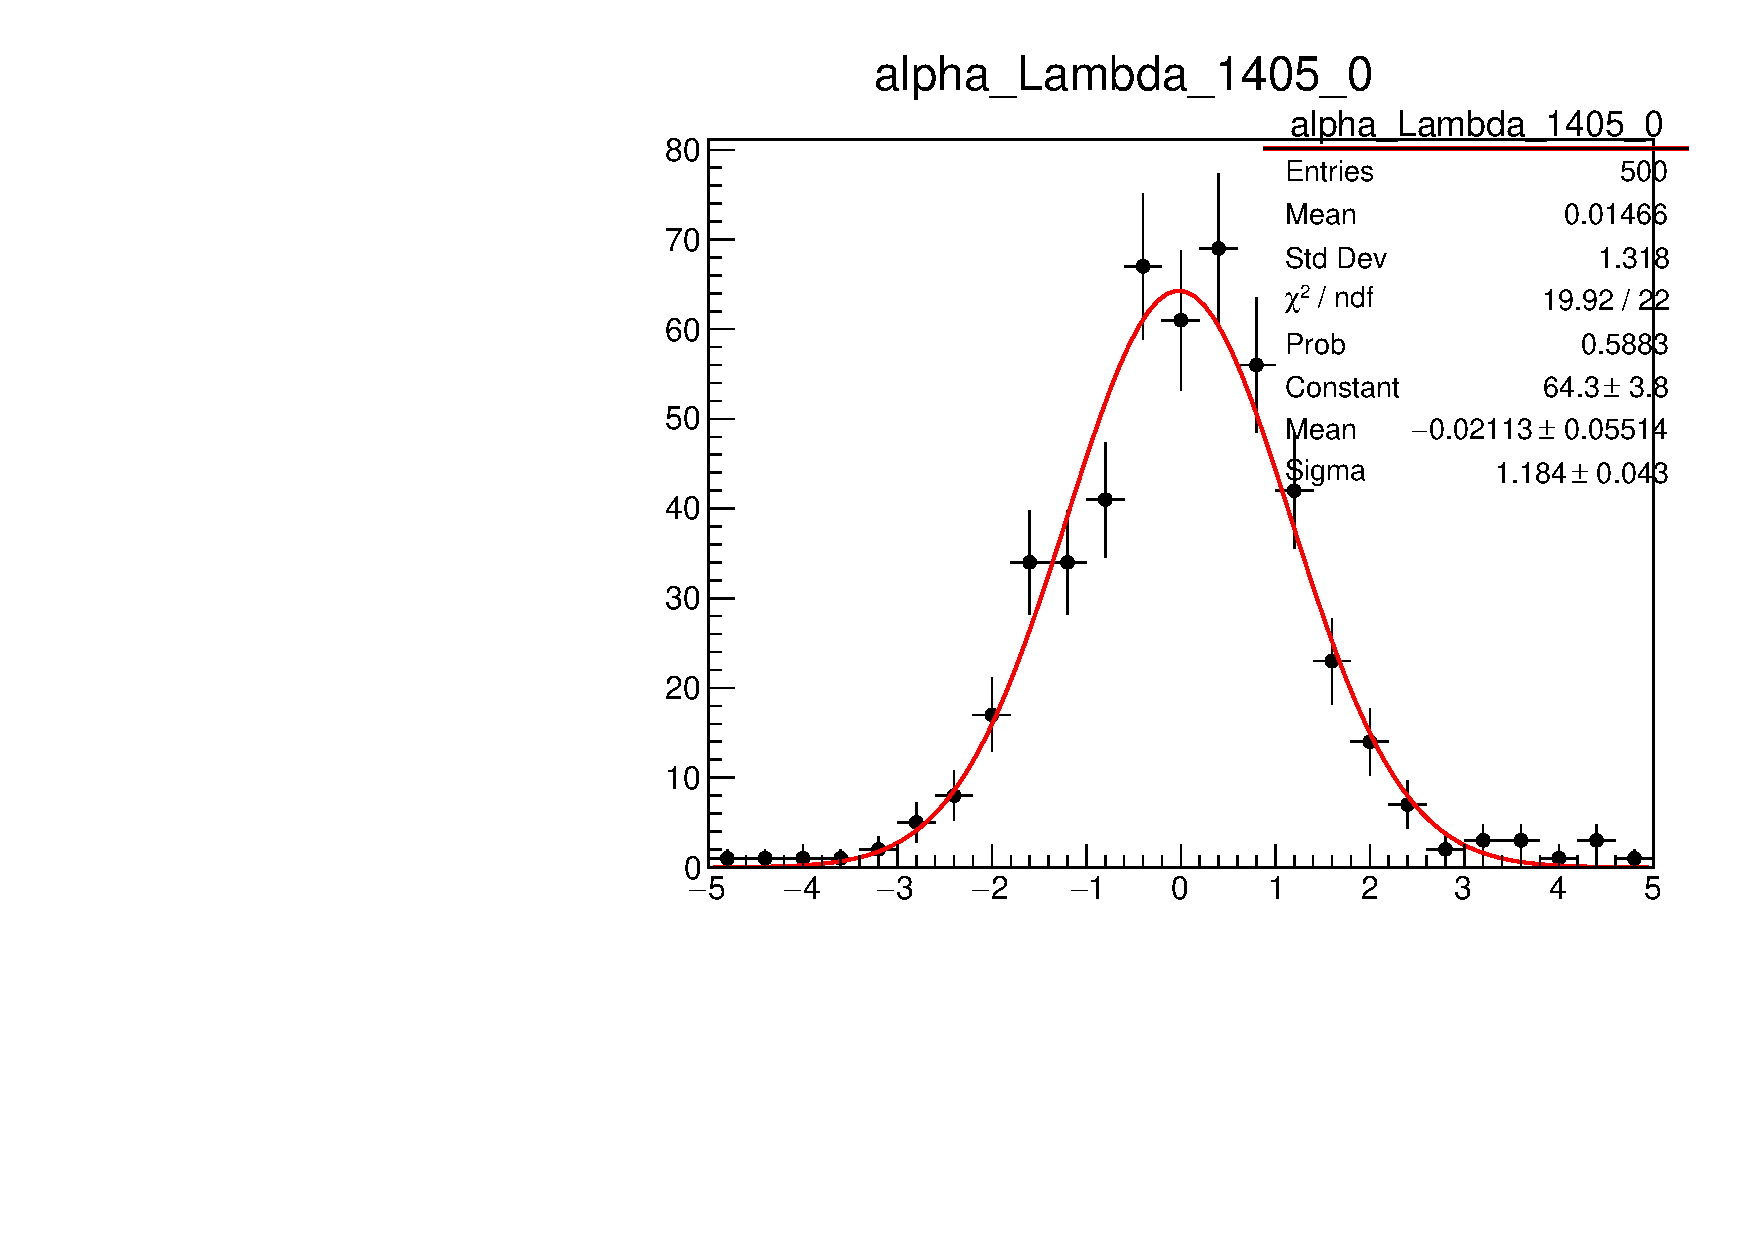
\includegraphics[width=0.24\textwidth]{figure/io_wo_bkg/alpha/pull_alpha_Lambda_1405_0.pdf}
    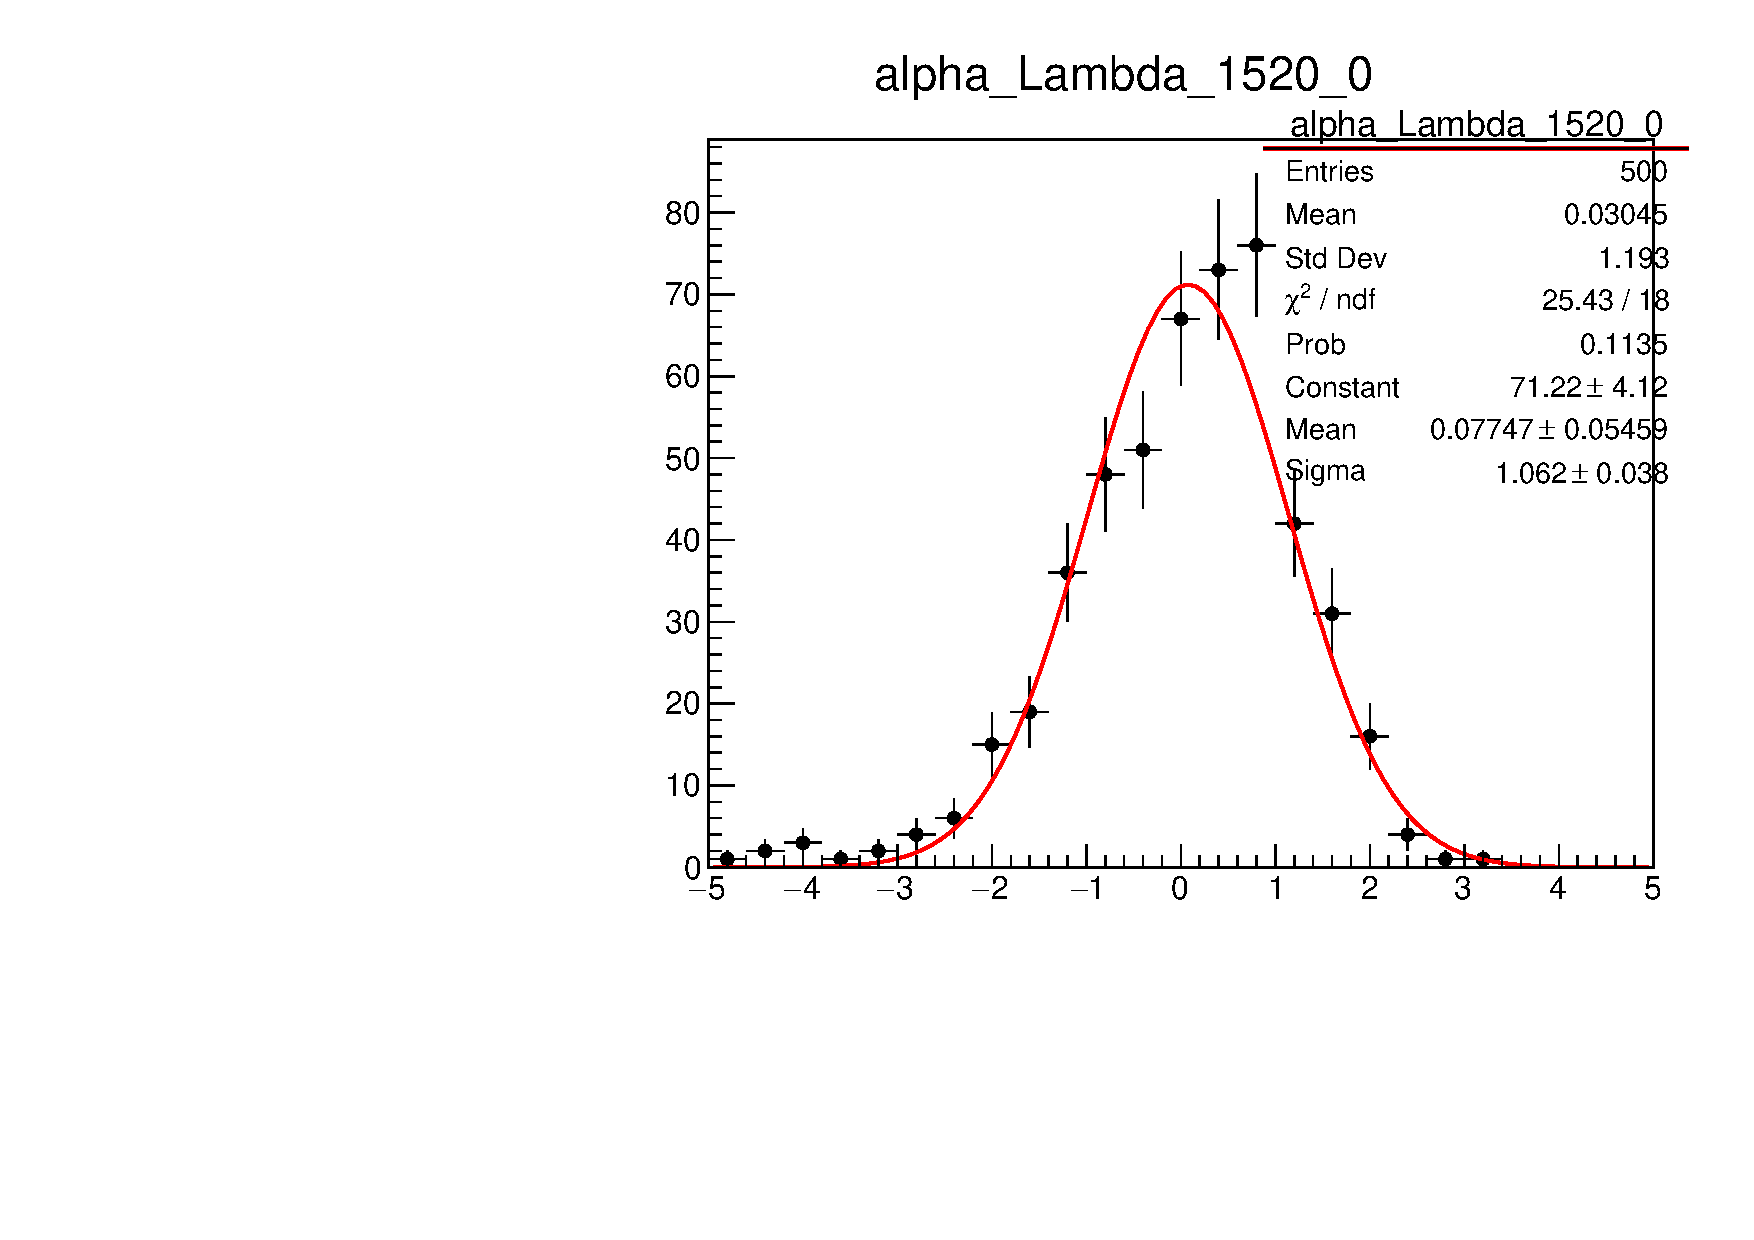
\includegraphics[width=0.24\textwidth]{figure/io_wo_bkg/alpha/pull_alpha_Lambda_1520_0.pdf}
    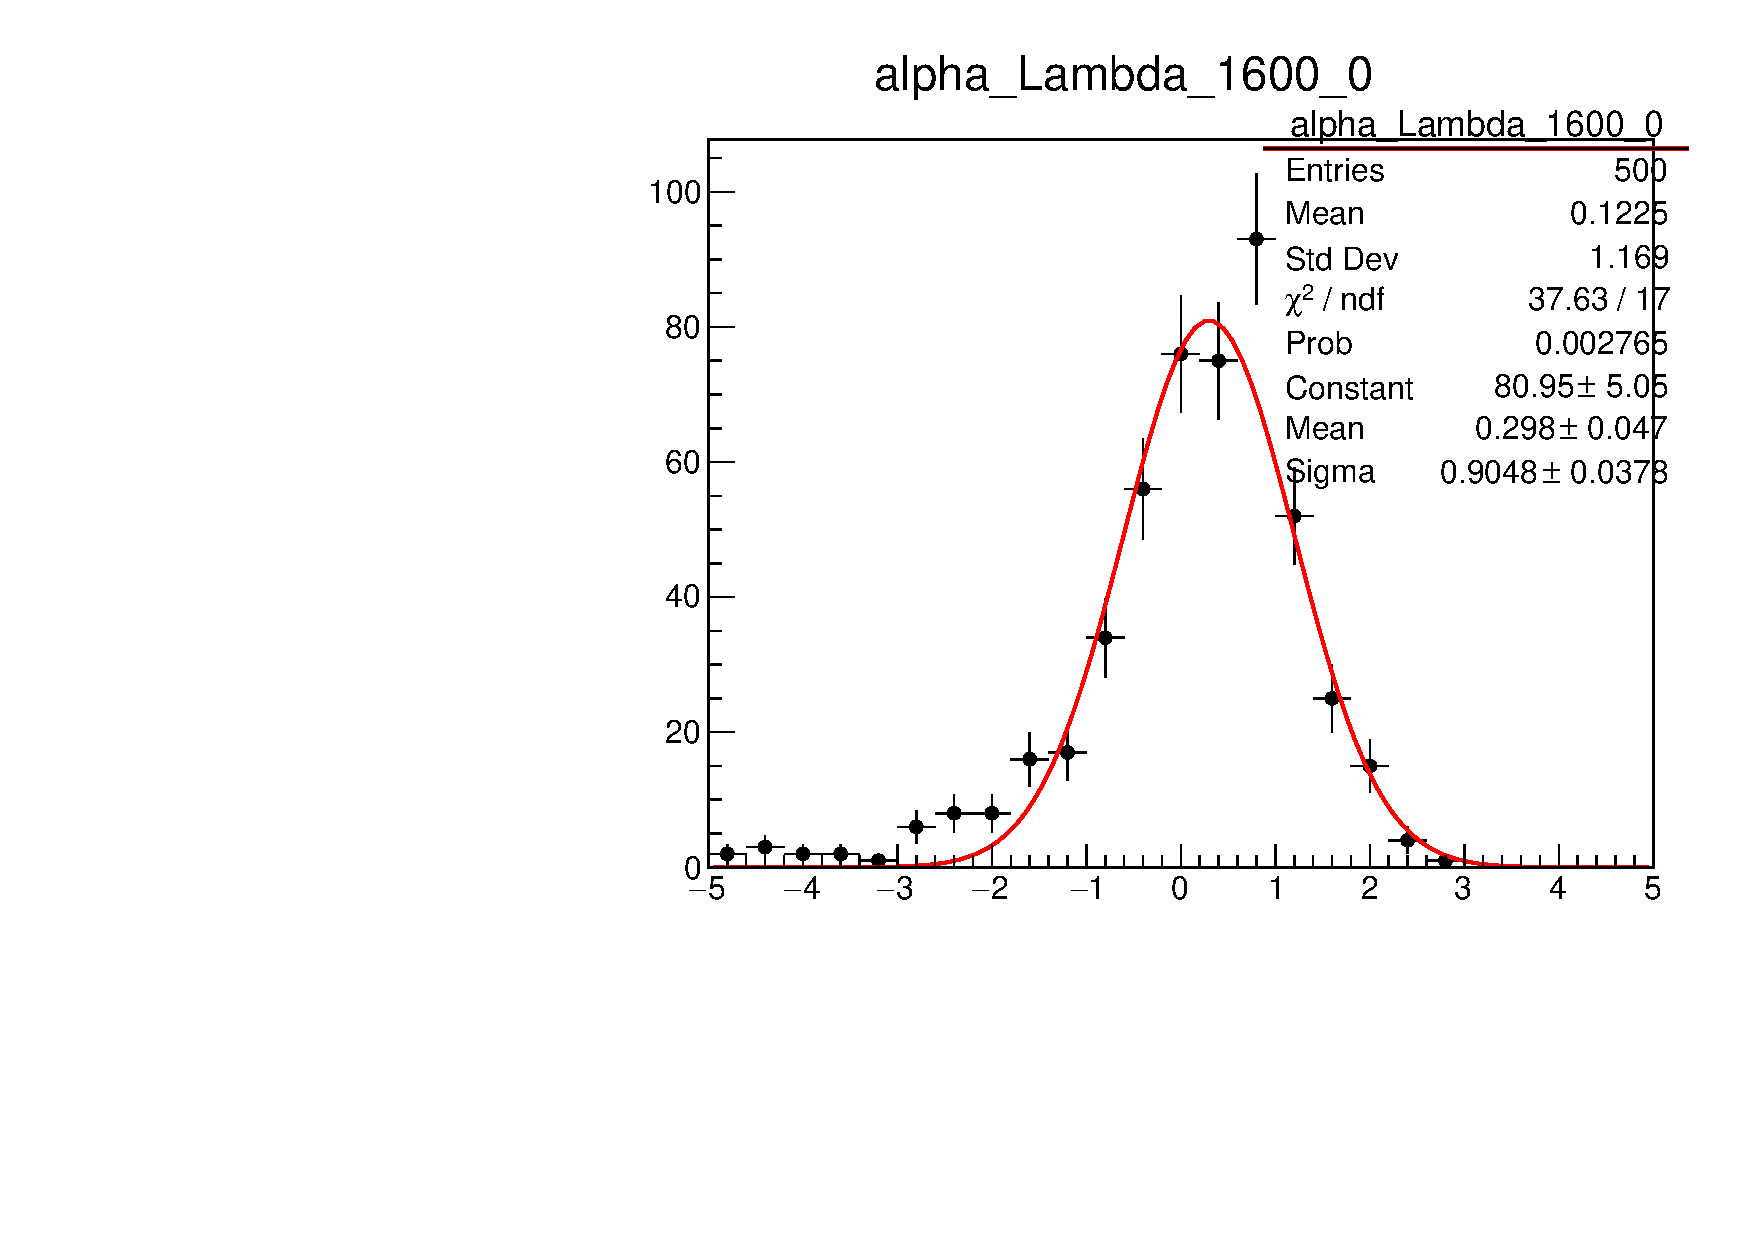
\includegraphics[width=0.24\textwidth]{figure/io_wo_bkg/alpha/pull_alpha_Lambda_1600_0.pdf}
    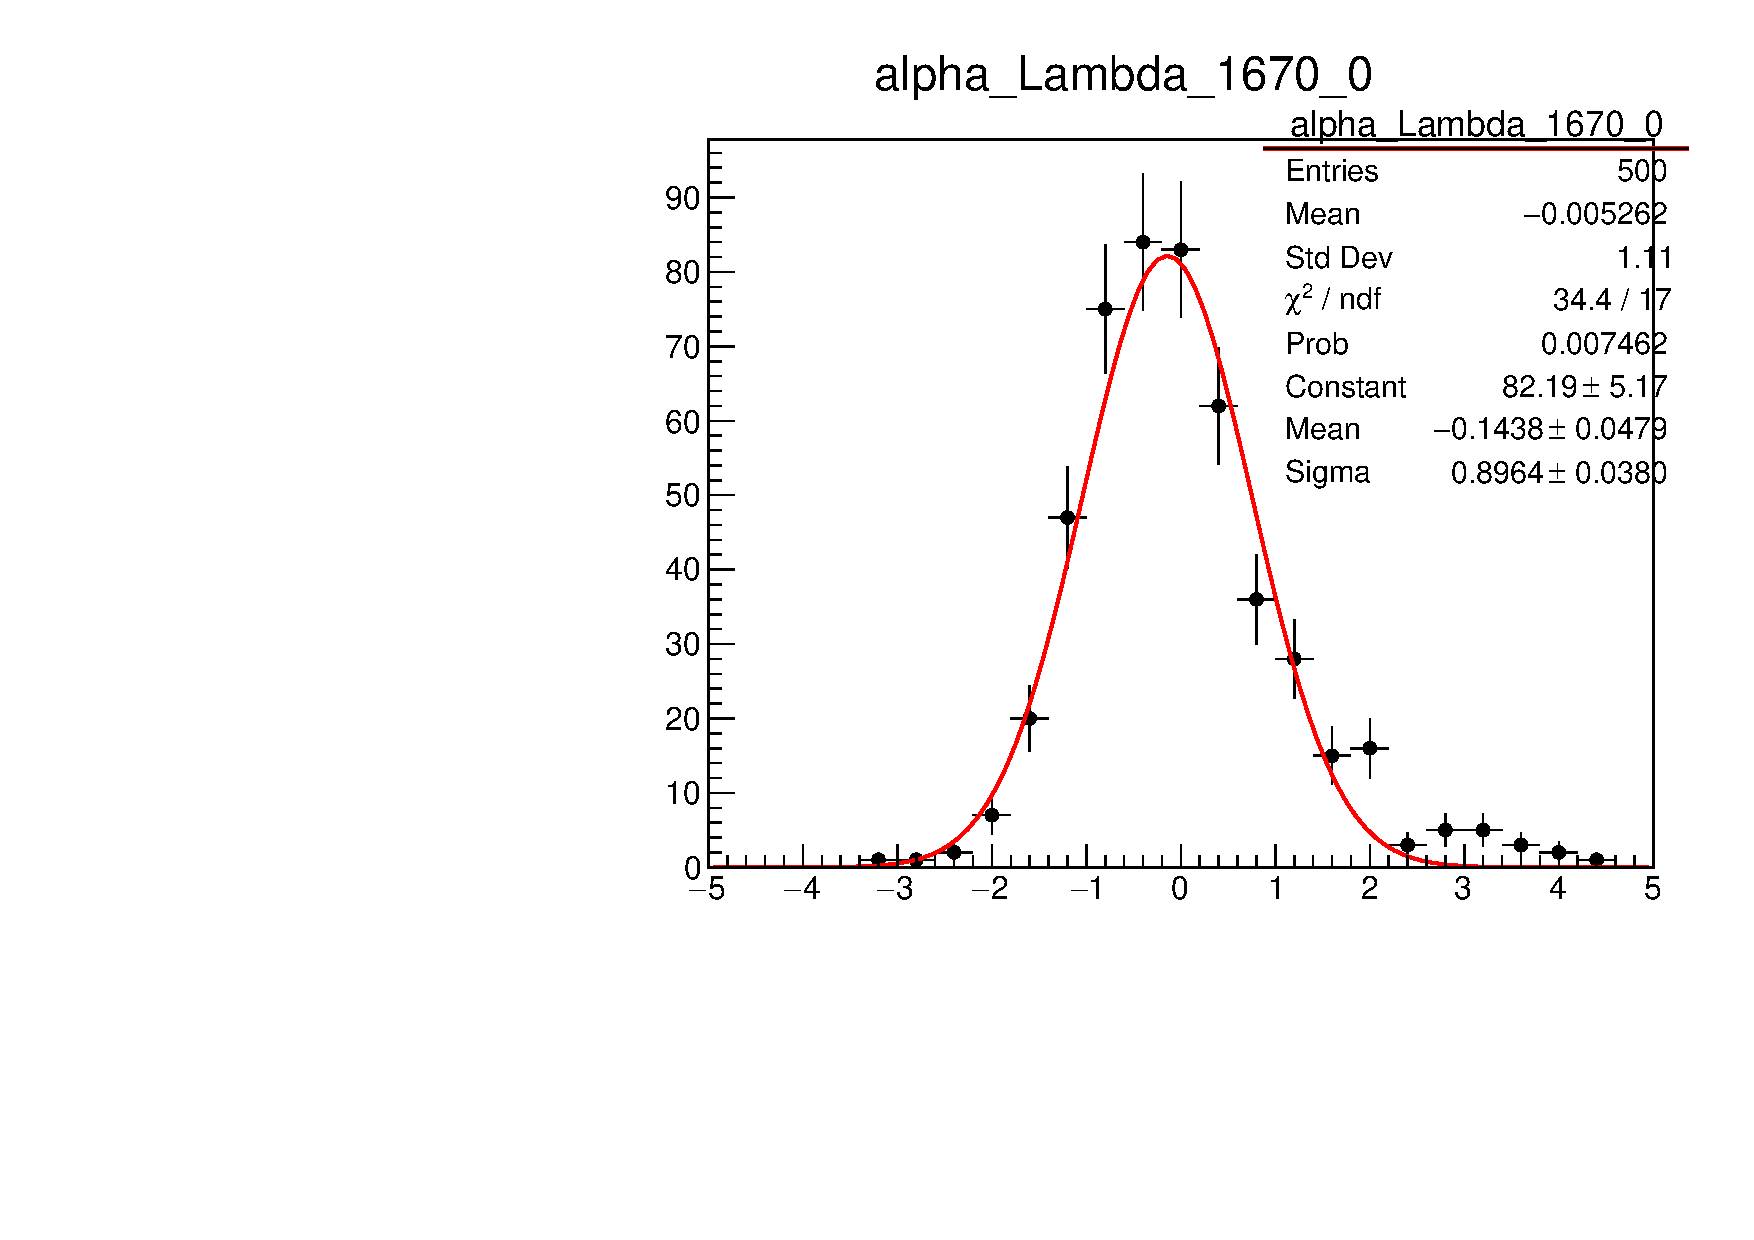
\includegraphics[width=0.24\textwidth]{figure/io_wo_bkg/alpha/pull_alpha_Lambda_1670_0.pdf}
    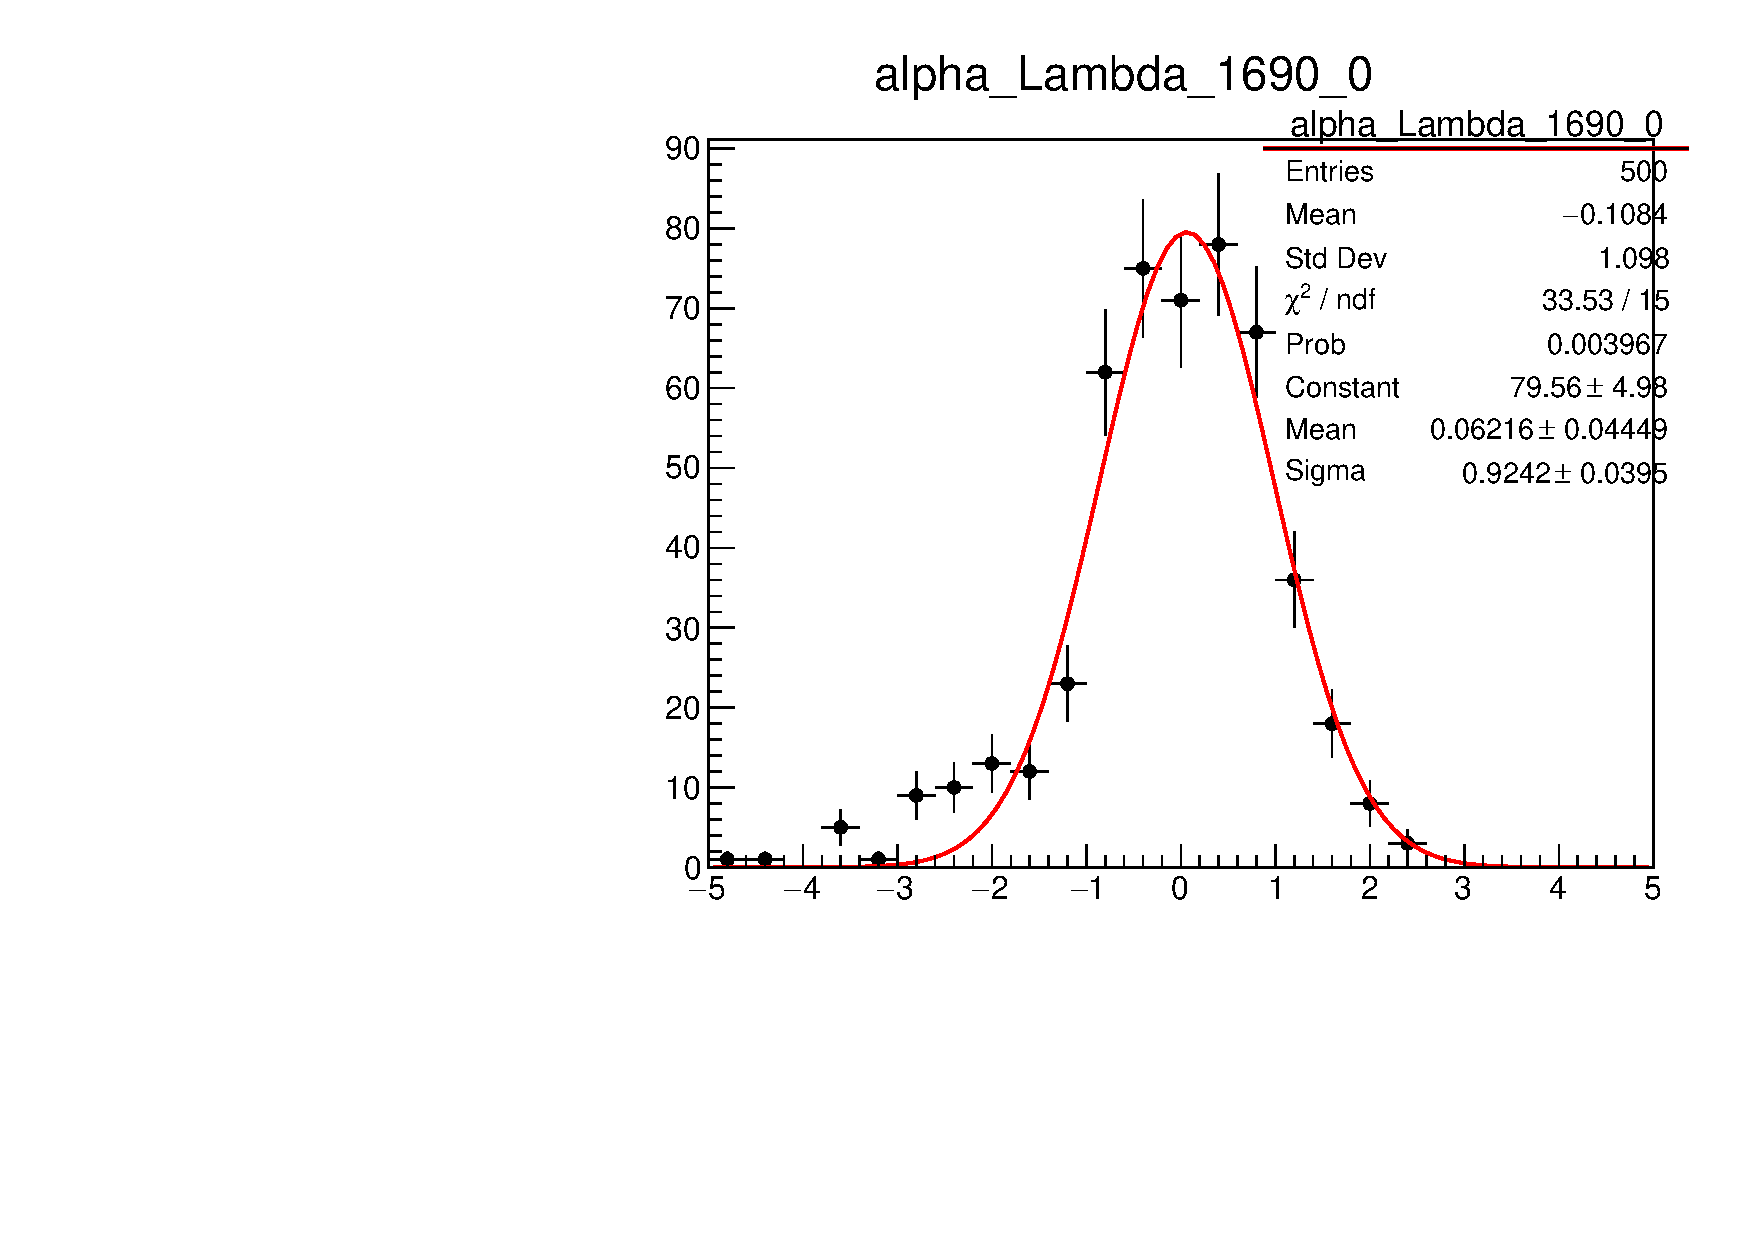
\includegraphics[width=0.24\textwidth]{figure/io_wo_bkg/alpha/pull_alpha_Lambda_1690_0.pdf}
    \includegraphics[width=0.24\textwidth]{figure/io_wo_bkg/alpha/pull_alpha_Lambda_2000_0.pdf}
    \includegraphics[width=0.24\textwidth]{figure/io_wo_bkg/alpha/pull_alpha_alpha_K_892_0.pdf}
    \includegraphics[width=0.24\textwidth]{figure/io_wo_bkg/alpha/pull_alpha_beta_K_892_0.pdf}
    \includegraphics[width=0.24\textwidth]{figure/io_wo_bkg/alpha/pull_alpha_gamma_K_892_0.pdf}
    \includegraphics[width=0.24\textwidth]{figure/io_wo_bkg/alpha/pull_alpha_lambda_K_892_0.pdf}
    \caption{Pull distributions for decay asymmetry parameters.}
\label{fig:io_wo_bkg_pull_asymmetry}
\end{figure}

\begin{figure}[h]\centering
    \includegraphics[width=0.24\textwidth]{figure/io_wo_bkg/gls/pull_gls_epem4600_Lmdc.aLmdc_g_ls_1r.pdf}
    \includegraphics[width=0.24\textwidth]{figure/io_wo_bkg/gls/pull_gls_epem4612_Lmdc.aLmdc_g_ls_1r.pdf}
    \includegraphics[width=0.24\textwidth]{figure/io_wo_bkg/gls/pull_gls_epem4626_Lmdc.aLmdc_g_ls_1r.pdf}
    \includegraphics[width=0.24\textwidth]{figure/io_wo_bkg/gls/pull_gls_epem4640_Lmdc.aLmdc_g_ls_1r.pdf}
    \includegraphics[width=0.24\textwidth]{figure/io_wo_bkg/gls/pull_gls_epem4660_Lmdc.aLmdc_g_ls_1r.pdf}
    \includegraphics[width=0.24\textwidth]{figure/io_wo_bkg/gls/pull_gls_epem4680_Lmdc.aLmdc_g_ls_1r.pdf}
    \includegraphics[width=0.24\textwidth]{figure/io_wo_bkg/gls/pull_gls_epem4700_Lmdc.aLmdc_g_ls_1r.pdf}
    \includegraphics[width=0.24\textwidth]{figure/io_wo_bkg/gls/pull_gls_epem4740_Lmdc.aLmdc_g_ls_1r.pdf}
    \includegraphics[width=0.24\textwidth]{figure/io_wo_bkg/gls/pull_gls_epem4750_Lmdc.aLmdc_g_ls_1r.pdf}
    \includegraphics[width=0.24\textwidth]{figure/io_wo_bkg/gls/pull_gls_epem4780_Lmdc.aLmdc_g_ls_1r.pdf}
    \includegraphics[width=0.24\textwidth]{figure/io_wo_bkg/gls/pull_gls_epem4840_Lmdc.aLmdc_g_ls_1r.pdf}
    \includegraphics[width=0.24\textwidth]{figure/io_wo_bkg/gls/pull_gls_epem4914_Lmdc.aLmdc_g_ls_1r.pdf}
    \includegraphics[width=0.24\textwidth]{figure/io_wo_bkg/gls/pull_gls_epem4946_Lmdc.aLmdc_g_ls_1r.pdf}
    \caption{Pull distributions for amplitude magnitudes of $e^+e^-\to\lcp\lcm$.}
\label{fig:io_wo_bkg_pull_magnitudes}
\end{figure}

\begin{figure}[h]\centering
    \includegraphics[width=0.24\textwidth]{figure/io_wo_bkg/gls/pull_gls_epem4600_Lmdc.aLmdc_g_ls_1i.pdf}
    \includegraphics[width=0.24\textwidth]{figure/io_wo_bkg/gls/pull_gls_epem4612_Lmdc.aLmdc_g_ls_1i.pdf}
    \includegraphics[width=0.24\textwidth]{figure/io_wo_bkg/gls/pull_gls_epem4626_Lmdc.aLmdc_g_ls_1i.pdf}
    \includegraphics[width=0.24\textwidth]{figure/io_wo_bkg/gls/pull_gls_epem4640_Lmdc.aLmdc_g_ls_1i.pdf}
    \includegraphics[width=0.24\textwidth]{figure/io_wo_bkg/gls/pull_gls_epem4660_Lmdc.aLmdc_g_ls_1i.pdf}
    \includegraphics[width=0.24\textwidth]{figure/io_wo_bkg/gls/pull_gls_epem4680_Lmdc.aLmdc_g_ls_1i.pdf}
    \includegraphics[width=0.24\textwidth]{figure/io_wo_bkg/gls/pull_gls_epem4700_Lmdc.aLmdc_g_ls_1i.pdf}
    \includegraphics[width=0.24\textwidth]{figure/io_wo_bkg/gls/pull_gls_epem4740_Lmdc.aLmdc_g_ls_1i.pdf}
    \includegraphics[width=0.24\textwidth]{figure/io_wo_bkg/gls/pull_gls_epem4750_Lmdc.aLmdc_g_ls_1i.pdf}
    \includegraphics[width=0.24\textwidth]{figure/io_wo_bkg/gls/pull_gls_epem4780_Lmdc.aLmdc_g_ls_1i.pdf}
    \includegraphics[width=0.24\textwidth]{figure/io_wo_bkg/gls/pull_gls_epem4840_Lmdc.aLmdc_g_ls_1i.pdf}
    \includegraphics[width=0.24\textwidth]{figure/io_wo_bkg/gls/pull_gls_epem4914_Lmdc.aLmdc_g_ls_1i.pdf}
    \includegraphics[width=0.24\textwidth]{figure/io_wo_bkg/gls/pull_gls_epem4946_Lmdc.aLmdc_g_ls_1i.pdf}
    \caption{Pull distributions for amplitude phases of $e^+e^-\to\lcp\lcm$.}
\label{fig:io_wo_bkg_pull_phase}
\end{figure}

\begin{table}[h]
    \caption{Fit results of pull distributions for $\alpha_0$ and $\Delta_0$ for each energy point.}
    \label{tab:fit_io_wo_bkg_pull_polarization}
    \resizebox{\textwidth}{!}{
        \begin{tabular}{cccccc}
            \hline\hline
        dataSet & $\mu_{\rm pull}$ & $\sigma_{\rm pull}$ & Nominal & Corrected & Difference \\\hline
        \multicolumn{6}{c}{$\alpha_0$} \\\hline
        4600 & -0.072 $\pm$ 0.046 & 1.021 $\pm$ 0.032 & -0.249 $\pm$ 0.036 & -0.252 $\pm$ 0.037 & 0.003\\
        4612 & -0.095 $\pm$ 0.046 & 1.021 $\pm$ 0.032 & -0.243 $\pm$ 0.092 & -0.252 $\pm$ 0.094 & 0.009\\
        4626 & -0.150 $\pm$ 0.045 & 1.005 $\pm$ 0.032 & -0.191 $\pm$ 0.042 & -0.197 $\pm$ 0.042 & 0.006\\
        4640 & -0.034 $\pm$ 0.046 & 1.035 $\pm$ 0.033 & -0.083 $\pm$ 0.045 & -0.085 $\pm$ 0.047 & 0.002\\
        4660 & 0.031 $\pm$ 0.048 & 1.069 $\pm$ 0.034 & -0.009 $\pm$ 0.050 & -0.008 $\pm$ 0.053 & 0.002\\
        4680 & -0.042 $\pm$ 0.048 & 1.078 $\pm$ 0.034 & 0.116 $\pm$ 0.032 & 0.114 $\pm$ 0.035 & 0.001\\
        4700 & -0.047 $\pm$ 0.045 & 1.016 $\pm$ 0.032 & 0.318 $\pm$ 0.069 & 0.315 $\pm$ 0.070 & 0.003\\
        4740 & -0.067 $\pm$ 0.047 & 1.057 $\pm$ 0.033 & 0.421 $\pm$ 0.159 & 0.409 $\pm$ 0.169 & 0.011\\
        4750 & -0.058 $\pm$ 0.046 & 1.030 $\pm$ 0.033 & 0.421 $\pm$ 0.104 & 0.415 $\pm$ 0.107 & 0.006\\
        4780 & -0.052 $\pm$ 0.046 & 1.021 $\pm$ 0.032 & 0.167 $\pm$ 0.077 & 0.163 $\pm$ 0.078 & 0.004\\
        4840 & 0.024 $\pm$ 0.044 & 0.978 $\pm$ 0.031 & 0.334 $\pm$ 0.107 & 0.337 $\pm$ 0.104 & 0.002\\
        4920 & -0.061 $\pm$ 0.053 & 1.167 $\pm$ 0.037 & 0.697 $\pm$ 0.196 & 0.683 $\pm$ 0.229 & 0.014\\
        4950 & -0.038 $\pm$ 0.046 & 1.020 $\pm$ 0.032 & 0.447 $\pm$ 0.215 & 0.439 $\pm$ 0.220 & 0.008\\\hline
        \multicolumn{6}{c}{$\sin\Delta_0$} \\\hline
        4600 & -0.116 $\pm$ 0.049 & 1.093 $\pm$ 0.035 & -0.224 $\pm$ 0.084 & -0.235 $\pm$ 0.092 & 0.011\\
        4612 & -0.070 $\pm$ 0.044 & 0.991 $\pm$ 0.031 & -0.463 $\pm$ 0.211 & -0.478 $\pm$ 0.209 & 0.015\\
        4626 & -0.016 $\pm$ 0.046 & 1.030 $\pm$ 0.033 & -0.244 $\pm$ 0.099 & -0.246 $\pm$ 0.102 & 0.002\\
        4640 & -0.103 $\pm$ 0.048 & 1.083 $\pm$ 0.034 & -0.438 $\pm$ 0.096 & -0.449 $\pm$ 0.104 & 0.011\\
        4660 & -0.065 $\pm$ 0.048 & 1.067 $\pm$ 0.034 & -0.515 $\pm$ 0.099 & -0.522 $\pm$ 0.106 & 0.007\\
        4680 & -0.088 $\pm$ 0.048 & 1.082 $\pm$ 0.034 & -0.425 $\pm$ 0.064 & -0.432 $\pm$ 0.069 & 0.006\\
        4700 & -0.099 $\pm$ 0.047 & 1.045 $\pm$ 0.033 & -0.585 $\pm$ 0.135 & -0.599 $\pm$ 0.142 & 0.014\\
        4740 & 0.032 $\pm$ 0.044 & 0.977 $\pm$ 0.031 & 0.281 $\pm$ 0.298 & 0.290 $\pm$ 0.291 & 0.009\\
        4750 & -0.052 $\pm$ 0.046 & 1.032 $\pm$ 0.033 & -0.424 $\pm$ 0.210 & -0.436 $\pm$ 0.216 & 0.011\\
        4780 & -0.119 $\pm$ 0.048 & 1.084 $\pm$ 0.034 & -0.433 $\pm$ 0.149 & -0.453 $\pm$ 0.162 & 0.019\\
        4840 & -0.020 $\pm$ 0.046 & 1.031 $\pm$ 0.033 & -0.429 $\pm$ 0.217 & -0.433 $\pm$ 0.223 & 0.004\\
        4920 & -0.220 $\pm$ 0.041 & 0.841 $\pm$ 0.029 & 0.351 $\pm$ 0.446 & 0.268 $\pm$ 0.375 & 0.082\\
        4950 & 0.096 $\pm$ 0.044 & 0.952 $\pm$ 0.031 & -0.223 $\pm$ 0.405 & -0.186 $\pm$ 0.385 & 0.037\\
        \hline\hline
        \end{tabular}
        }
\end{table}

\begin{table}[h]
    \caption{Fit results of pull distributions for FF of each resonance.}
    \label{tab:fit_io_wo_bkg_pull_ff}
    \resizebox{\textwidth}{!}{
        \begin{tabular}{cccccc}
            \hline\hline
            Resonance & $\mu_{\text{pull}}$ & $\sigma_{\text{pull}}$ & Nominal FF (\%) & Corrected FF (\%) & Difference (\%)\\\hline
            $\Delta(1232)^{++}$ & -0.11$\pm$0.05 & 1.06$\pm$0.03 & 27.34$\pm$1.03 & 27.46$\pm$1.10 & -0.12\\
            $\Delta(1600)^{++}$ & -0.03$\pm$0.05 & 1.08$\pm$0.05 & 7.68$\pm$2.02 & 7.74$\pm$2.17 & -0.05\\
            $\Delta(1600)^{++}$ & 0.10$\pm$0.05 & 1.04$\pm$0.04 & 5.42$\pm$1.89 & 5.23$\pm$1.97 & 0.19\\
            $\Delta(1700)^{++}$ & -0.26$\pm$0.05 & 1.04$\pm$0.04 & 12.74$\pm$1.42 & 13.12$\pm$1.47 & -0.38\\
            $K_{0}^{*}(1430)$ & 0.07$\pm$0.05 & 1.09$\pm$0.04 & 13.67$\pm$2.61 & 13.46$\pm$2.84 & 0.21\\
            $K_{0}^{*}(700)$ & 0.26$\pm$0.05 & 1.05$\pm$0.05 & 2.90$\pm$0.67 & 2.72$\pm$0.70 & 0.18\\
            $K^{*}(892)$ & -0.48$\pm$0.05 & 0.99$\pm$0.03 & 24.98$\pm$0.99 & 25.45$\pm$0.98 & -0.47\\
            $\Lambda(1405)$ & 0.11$\pm$0.05 & 0.90$\pm$0.03 & 4.35$\pm$1.09 & 4.24$\pm$0.98 & 0.11\\
            $\Lambda(1520)$ & 0.33$\pm$0.05 & 0.97$\pm$0.03 & 1.10$\pm$0.17 & 1.05$\pm$0.16 & 0.05\\
            $\Lambda(1600)$ & -0.03$\pm$0.05 & 0.99$\pm$0.03 & 5.56$\pm$1.15 & 5.59$\pm$1.14 & -0.03\\
            $\Lambda(1670)$ & 0.27$\pm$0.05 & 0.99$\pm$0.03 & 1.68$\pm$0.26 & 1.61$\pm$0.26 & 0.07\\
            $\Lambda(1690)$ & 0.16$\pm$0.05 & 0.93$\pm$0.04 & 1.07$\pm$0.26 & 1.03$\pm$0.24 & 0.04\\
            $\Lambda(2000)$ & 0.22$\pm$0.05 & 1.00$\pm$0.03 & 5.94$\pm$0.51 & 5.83$\pm$0.51 & 0.11\\\hline
            Sum& & & 114.45$\pm$4.68 & 114.53$\pm$4.91 & \\
        \hline\hline
        \end{tabular}
        }
\end{table}


\begin{table}[h]
    \caption{Fit results of pull distributions for decay asymmetry parameters.}
    \label{tab:fit_io_wo_bkg_pull_alpha}
    \resizebox{\textwidth}{!}{
        \begin{tabular}{cccccc}
            \hline\hline
            Parameters & $\mu_{\text{pull}}$ & $\sigma_{\text{pull}}$ & Nominal & Corrected & Difference\\\hline
            $\alpha_{\Lambda_c^+}^{\pi^{+}\Lambda(1520)}$ & 0.077$\pm$0.055 & 1.062$\pm$0.038 & -0.551$\pm$0.243 & -0.531$\pm$0.259 & 0.020\\
            $\alpha_{\Lambda_c^+}^{\pi^{+}\Lambda(1690)}$ & 0.062$\pm$0.044 & 0.924$\pm$0.039 & -0.802$\pm$0.160 & -0.793$\pm$0.148 & 0.009\\
            $\alpha_{\Lambda_c^+}^{K^{-}\Delta(1232)^{++}}$ & -0.016$\pm$0.047 & 1.012$\pm$0.038 & -0.669$\pm$0.099 & -0.671$\pm$0.100 & 0.002\\
            $\alpha_{\Lambda_c^+}^{K^{-}\Delta(1600)^{++}}$ & 0.105$\pm$0.050 & 1.091$\pm$0.039 & -0.027$\pm$0.223 & -0.002$\pm$0.243 & 0.025\\
            $\alpha_{\Lambda_c^+}^{K^{-}\Delta(1700)^{++}}$ & -0.141$\pm$0.047 & 1.034$\pm$0.038 & -0.159$\pm$0.075 & -0.170$\pm$0.077 & 0.011\\
            $\alpha_{\Lambda_c^+}^{\pi^{+}\Lambda(1405)}$ & -0.021$\pm$0.055 & 1.184$\pm$0.043 & 0.000$\pm$0.458 & -0.011$\pm$0.543 & 0.011\\
            $\alpha_{\Lambda_c^+}^{\pi^{+}\Lambda(1600)}$ & 0.298$\pm$0.047 & 0.905$\pm$0.038 & -0.834$\pm$0.106 & -0.805$\pm$0.096 & 0.029\\
            $\alpha_{\Lambda_c^+}^{\pi^{+}\Lambda(1670)}$ & -0.144$\pm$0.048 & 0.896$\pm$0.038 & 0.803$\pm$0.199 & 0.778$\pm$0.178 & 0.026\\
            $\alpha_{\Lambda_c^+}^{\pi^{+}\Lambda(2000)}$ & 0.035$\pm$0.055 & 0.969$\pm$0.038 & -0.833$\pm$0.094 & -0.830$\pm$0.091 & 0.003\\
            $\alpha_{\Lambda_c^+}^{K^{-}\Delta(1620)^{++}}$ & 0.059$\pm$0.052 & 1.133$\pm$0.038 & -0.028$\pm$0.302 & -0.008$\pm$0.342 & 0.020\\
            $\alpha_{\Lambda_c^+}^{p\overline{K}^*_0(700)}$ & -0.042$\pm$0.055 & 1.157$\pm$0.044 & 0.216$\pm$0.270 & 0.203$\pm$0.313 & 0.013\\
            $\alpha_{\Lambda_c^+}^{p\overline{K}^*_0(1430)}$ & -0.169$\pm$0.049 & 1.065$\pm$0.036 & -0.202$\pm$0.072 & -0.215$\pm$0.076 & 0.013\\
            $\alpha_{\Lambda_c^+}^{p\overline{K}^*(892)}$ & 0.204$\pm$0.048 & 1.020$\pm$0.036 & -0.773$\pm$0.091 & -0.754$\pm$0.093 & 0.019\\
            $\beta_{\Lambda_c^+}^{p\overline{K}^*(892)}$ & -0.124$\pm$0.051 & 1.090$\pm$0.045 & -0.402$\pm$0.206 & -0.430$\pm$0.224 & 0.028\\
            $\gamma_{\Lambda_c^+}^{p\overline{K}^*(892)}$ & 0.004$\pm$0.048 & 1.021$\pm$0.042 & 1.503$\pm$0.159 & 1.503$\pm$0.162 & 0.001\\
            $\Lambda_{\Lambda_c^+}^{p\overline{K}^*(892)}$ & 0.102$\pm$0.046 & 0.969$\pm$0.038 & -0.625$\pm$0.083 & -0.617$\pm$0.081 & 0.008\\
        \hline\hline
        \end{tabular}
        }
\end{table}

\begin{table}[h]
    \caption{Fit results of pull distributions for amplitude magnitudes and phases of $e^+e^-\to\lcp\lcm$.}
    \label{tab:fit_io_wo_bkg_pull_gls}
    \resizebox{\textwidth}{!}{
        \begin{tabular}{cccccc}
        \hline\hline
        Parameters & $\mu_{\text{pull}}$ & $\sigma_{\text{pull}}$ & Nominal & Corrected & Difference (\%)\\\hline
epem4600$->$Lmdc.aLmdc$\_$g$\_$ls$\_$1i & 0.11$\pm$0.06 & 1.06$\pm$0.06 & -2.39$\pm$0.22 & -2.41$\pm$0.23 & 0.03 \\
epem4600$->$Lmdc.aLmdc$\_$g$\_$ls$\_$1r & 0.19$\pm$0.05 & 0.96$\pm$0.04 & 0.17$\pm$0.03 & 0.16$\pm$0.03 & 0.01 \\
epem4612$->$Lmdc.aLmdc$\_$g$\_$ls$\_$1i & 0.23$\pm$0.05 & 0.87$\pm$0.04 & -1.98$\pm$0.29 & -2.04$\pm$0.26 & 0.06 \\
epem4612$->$Lmdc.aLmdc$\_$g$\_$ls$\_$1r & -0.04$\pm$0.04 & 0.78$\pm$0.03 & 0.27$\pm$0.11 & 0.27$\pm$0.09 & -0.00 \\
epem4626$->$Lmdc.aLmdc$\_$g$\_$ls$\_$1i & -0.08$\pm$0.05 & 1.05$\pm$0.04 & -0.48$\pm$0.18 & -0.47$\pm$0.18 & -0.01 \\
epem4626$->$Lmdc.aLmdc$\_$g$\_$ls$\_$1r & -0.04$\pm$0.05 & 1.00$\pm$0.03 & 3.55$\pm$0.40 & 3.56$\pm$0.40 & -0.02 \\
epem4640$->$Lmdc.aLmdc$\_$g$\_$ls$\_$1i & -0.15$\pm$0.05 & 1.07$\pm$0.04 & -0.67$\pm$0.12 & -0.65$\pm$0.13 & -0.02 \\
epem4640$->$Lmdc.aLmdc$\_$g$\_$ls$\_$1r & -0.17$\pm$0.05 & 1.01$\pm$0.03 & 2.55$\pm$0.28 & 2.60$\pm$0.28 & -0.05 \\
epem4660$->$Lmdc.aLmdc$\_$g$\_$ls$\_$1i & 0.15$\pm$0.05 & 1.09$\pm$0.03 & -1.50$\pm$0.10 & -1.51$\pm$0.11 & 0.02 \\
epem4660$->$Lmdc.aLmdc$\_$g$\_$ls$\_$1r & 0.08$\pm$0.05 & 1.10$\pm$0.04 & 0.26$\pm$0.06 & 0.26$\pm$0.06 & 0.01 \\
epem4680$->$Lmdc.aLmdc$\_$g$\_$ls$\_$1i & -0.10$\pm$0.05 & 1.06$\pm$0.04 & -0.51$\pm$0.07 & -0.51$\pm$0.07 & -0.01 \\
epem4680$->$Lmdc.aLmdc$\_$g$\_$ls$\_$1r & -0.07$\pm$0.05 & 1.03$\pm$0.04 & 2.08$\pm$0.12 & 2.09$\pm$0.12 & -0.01 \\
epem4700$->$Lmdc.aLmdc$\_$g$\_$ls$\_$1i & -0.14$\pm$0.05 & 1.05$\pm$0.03 & -0.55$\pm$0.12 & -0.53$\pm$0.12 & -0.02 \\
epem4700$->$Lmdc.aLmdc$\_$g$\_$ls$\_$1r & -0.06$\pm$0.04 & 0.93$\pm$0.03 & 1.57$\pm$0.18 & 1.58$\pm$0.17 & -0.01 \\
epem4740$->$Lmdc.aLmdc$\_$g$\_$ls$\_$1i & 0.13$\pm$0.06 & 1.15$\pm$0.05 & 0.50$\pm$0.45 & 0.44$\pm$0.51 & 0.07 \\
epem4740$->$Lmdc.aLmdc$\_$g$\_$ls$\_$1r & 0.14$\pm$0.04 & 0.70$\pm$0.03 & 0.23$\pm$0.10 & 0.22$\pm$0.07 & 0.01 \\
epem4750$->$Lmdc.aLmdc$\_$g$\_$ls$\_$1i & -0.08$\pm$0.05 & 1.03$\pm$0.03 & -0.36$\pm$0.17 & -0.34$\pm$0.18 & -0.01 \\
epem4750$->$Lmdc.aLmdc$\_$g$\_$ls$\_$1r & -0.09$\pm$0.05 & 0.96$\pm$0.03 & 1.56$\pm$0.21 & 1.58$\pm$0.20 & -0.02 \\
epem4780$->$Lmdc.aLmdc$\_$g$\_$ls$\_$1i & -0.11$\pm$0.05 & 1.03$\pm$0.04 & -0.49$\pm$0.16 & -0.47$\pm$0.16 & -0.02 \\
epem4780$->$Lmdc.aLmdc$\_$g$\_$ls$\_$1r & -0.14$\pm$0.05 & 1.05$\pm$0.04 & 1.97$\pm$0.24 & 2.01$\pm$0.26 & -0.04 \\
epem4840$->$Lmdc.aLmdc$\_$g$\_$ls$\_$1i & -0.02$\pm$0.05 & 1.02$\pm$0.04 & -0.81$\pm$0.25 & -0.81$\pm$0.26 & -0.00 \\
epem4840$->$Lmdc.aLmdc$\_$g$\_$ls$\_$1r & -0.02$\pm$0.05 & 0.93$\pm$0.04 & 0.25$\pm$0.09 & 0.25$\pm$0.09 & -0.00 \\
epem4914$->$Lmdc.aLmdc$\_$g$\_$ls$\_$1i & -0.02$\pm$0.05 & 0.99$\pm$0.04 & 0.20$\pm$0.24 & 0.20$\pm$0.24 & -0.01 \\
epem4914$->$Lmdc.aLmdc$\_$g$\_$ls$\_$1r & -0.01$\pm$0.04 & 0.85$\pm$0.03 & 1.23$\pm$0.30 & 1.23$\pm$0.25 & -0.00 \\
epem4946$->$Lmdc.aLmdc$\_$g$\_$ls$\_$1i & 0.05$\pm$0.05 & 1.06$\pm$0.04 & -0.18$\pm$0.33 & -0.20$\pm$0.35 & 0.02 \\
epem4946$->$Lmdc.aLmdc$\_$g$\_$ls$\_$1r & -0.21$\pm$0.04 & 0.83$\pm$0.03 & 1.62$\pm$0.39 & 1.69$\pm$0.32 & -0.07 \\
        \hline\hline
        \end{tabular}
        }
\end{table}

\clearpage
\subsection{IO check with full simulation signal MC samples}

The previous two IO checks use truth signal MC samples without considering the detector response. Although the resolution have been studied to have negligible effects on the final results in Appendix~\ref{app:resolution}, it is also worth to using full simulation signal MC samples to perform an IO check. The signal MC samples at $\sqrt{s} = 4.682\gev/c^2$ are generated and reconstructed by the BesEvtGen package. The amplitude analysis is repeated and pull distributions are shown in Figure~\ref{fig:io_full_sim_pull_alpha0}-\ref{fig:io_full_sim_pull_gls}. The fit results of pull distributions are listed in Table~\ref{tab:fit_io_full_sim_pull_polarization}-\ref{tab:fit_io_full_sim_pull_gls}.


\begin{figure}[h]\centering
    \includegraphics[width=0.45\textwidth]{figure/io_full_sim/polarization/pull_polarization_alpha0_4680.pdf}
    \includegraphics[width=0.45\textwidth]{figure/io_full_sim/polarization/pull_polarization_delta0_4680.pdf}
    \caption{Pull distributions of $\alpha_0$ and $\sin(\Delta_0)$ at $\sqrt{s} = 4.682\gev/c^2$.}
\label{fig:io_full_sim_pull_alpha0}
\end{figure}

\begin{figure}[h]\centering
    \includegraphics[width=0.24\textwidth]{figure/io_full_sim/fitfrac/pull_fitfrac_res0_comb.pdf}
    \includegraphics[width=0.24\textwidth]{figure/io_full_sim/fitfrac/pull_fitfrac_res1_comb.pdf}
    \includegraphics[width=0.24\textwidth]{figure/io_full_sim/fitfrac/pull_fitfrac_res2_comb.pdf}
    \includegraphics[width=0.24\textwidth]{figure/io_full_sim/fitfrac/pull_fitfrac_res3_comb.pdf}
    \includegraphics[width=0.24\textwidth]{figure/io_full_sim/fitfrac/pull_fitfrac_res4_comb.pdf}
    \includegraphics[width=0.24\textwidth]{figure/io_full_sim/fitfrac/pull_fitfrac_res5_comb.pdf}
    \includegraphics[width=0.24\textwidth]{figure/io_full_sim/fitfrac/pull_fitfrac_res6_comb.pdf}
    \includegraphics[width=0.24\textwidth]{figure/io_full_sim/fitfrac/pull_fitfrac_res7_comb.pdf}
    \includegraphics[width=0.24\textwidth]{figure/io_full_sim/fitfrac/pull_fitfrac_res8_comb.pdf}
    \includegraphics[width=0.24\textwidth]{figure/io_full_sim/fitfrac/pull_fitfrac_res9_comb.pdf}
    \includegraphics[width=0.24\textwidth]{figure/io_full_sim/fitfrac/pull_fitfrac_res10_comb.pdf}
    \includegraphics[width=0.24\textwidth]{figure/io_full_sim/fitfrac/pull_fitfrac_res11_comb.pdf}
    \includegraphics[width=0.24\textwidth]{figure/io_full_sim/fitfrac/pull_fitfrac_res12_comb.pdf}
    \caption{Pull distributions of FF for each resonance at $\sqrt{s} = 4.682\gev/c^2$.}
\label{fig:io_full_sim_pull_ff}
\end{figure}

\begin{figure}[h]\centering
    \includegraphics[width=0.24\textwidth]{figure/io_full_sim/alpha/pull_alpha_Delta_1232_pp.pdf}
    \includegraphics[width=0.24\textwidth]{figure/io_full_sim/alpha/pull_alpha_Delta_1600_pp.pdf}
    \includegraphics[width=0.24\textwidth]{figure/io_full_sim/alpha/pull_alpha_Delta_1620_pp.pdf}
    \includegraphics[width=0.24\textwidth]{figure/io_full_sim/alpha/pull_alpha_Delta_1700_pp.pdf}
    \includegraphics[width=0.24\textwidth]{figure/io_full_sim/alpha/pull_alpha_K_1430_0.pdf}
    \includegraphics[width=0.24\textwidth]{figure/io_full_sim/alpha/pull_alpha_K_700_0.pdf}
    \includegraphics[width=0.24\textwidth]{figure/io_full_sim/alpha/pull_alpha_Lambda_1405_0.pdf}
    \includegraphics[width=0.24\textwidth]{figure/io_full_sim/alpha/pull_alpha_Lambda_1520_0.pdf}
    \includegraphics[width=0.24\textwidth]{figure/io_full_sim/alpha/pull_alpha_Lambda_1600_0.pdf}
    \includegraphics[width=0.24\textwidth]{figure/io_full_sim/alpha/pull_alpha_Lambda_1670_0.pdf}
    \includegraphics[width=0.24\textwidth]{figure/io_full_sim/alpha/pull_alpha_Lambda_1690_0.pdf}
    \includegraphics[width=0.24\textwidth]{figure/io_full_sim/alpha/pull_alpha_Lambda_2000_0.pdf}
    \includegraphics[width=0.24\textwidth]{figure/io_full_sim/alpha/pull_alpha_alpha_K_892_0.pdf}
    \includegraphics[width=0.24\textwidth]{figure/io_full_sim/alpha/pull_alpha_beta_K_892_0.pdf}
    \includegraphics[width=0.24\textwidth]{figure/io_full_sim/alpha/pull_alpha_gamma_K_892_0.pdf}
    \includegraphics[width=0.24\textwidth]{figure/io_full_sim/alpha/pull_alpha_lambda_K_892_0.pdf}
    \caption{Pull distributions for decay asymmetry parameters at $\sqrt{s} = 4.682\gev/c^2$.}
\label{fig:io_full_sim_pull_asymmetry}
\end{figure}

\begin{figure}[h]\centering
    \includegraphics[width=0.45\textwidth]{figure/io_full_sim/gls/pull_gls_epem4680_Lmdc.aLmdc_g_ls_1r.pdf}
    \includegraphics[width=0.45\textwidth]{figure/io_full_sim/gls/pull_gls_epem4680_Lmdc.aLmdc_g_ls_1i.pdf}
    \caption{Pull distributions for amplitude magnitudes and phases of $e^+e^-\to\lcp\lcm$ at $\sqrt{s} = 4.682\gev/c^2$.}
\label{fig:io_full_sim_pull_gls}
\end{figure}

\begin{table}[h]
    \caption{Fit results of pull distributions for $\alpha_0$ and $\Delta_0$ for each energy point.}
    \label{tab:fit_io_full_sim_pull_polarization}
    \resizebox{\textwidth}{!}{
        \begin{tabular}{cccccc}
            \hline\hline
        dataSet & $\mu_{\rm pull}$ & $\sigma_{\rm pull}$ & Nominal & Corrected & Difference \\\hline
        \multicolumn{6}{c}{$\alpha_0$} \\\hline
        4680 & -0.307 $\pm$ 0.089 & 1.081 $\pm$ 0.063 & 0.116 $\pm$ 0.032 & 0.105 $\pm$ 0.035 & 0.011\\\hline
        \multicolumn{6}{c}{$\sin\Delta_0$} \\\hline
        4680 & -0.118 $\pm$ 0.088 & 1.060 $\pm$ 0.062 & -0.425 $\pm$ 0.064 & -0.433 $\pm$ 0.068 & 0.008\\
        \hline\hline
        \end{tabular}
        }
\end{table}

\begin{table}[h]
    \caption{Fit results of pull distributions for FF of each resonance.}
    \label{tab:fit_io_full_sim_pull_ff}
    \resizebox{\textwidth}{!}{
        \begin{tabular}{cccccc}
            \hline\hline
            Resonance & $\mu_{\text{pull}}$ & $\sigma_{\text{pull}}$ & Nominal FF (\%) & Corrected FF (\%) & Difference (\%)\\\hline
            $\Delta(1232)^{++}$ & -0.08$\pm$0.08 & 0.98$\pm$0.07 & 27.46$\pm$1.03 & 27.54$\pm$1.01 & -0.08\\
            $\Delta(1600)^{++}$ & 0.28$\pm$0.09 & 1.01$\pm$0.08 & 7.69$\pm$2.01 & 7.11$\pm$2.04 & 0.58\\
            $\Delta(1600)^{++}$ & 0.37$\pm$0.08 & 0.98$\pm$0.08 & 5.42$\pm$1.88 & 4.73$\pm$1.85 & 0.69\\
            $\Delta(1700)^{++}$ & -0.17$\pm$0.07 & 0.84$\pm$0.06 & 12.73$\pm$1.41 & 12.93$\pm$1.18 & -0.20\\
            $K_{0}^{*}(1430)$ & 0.08$\pm$0.07 & 0.92$\pm$0.07 & 13.69$\pm$2.61 & 13.50$\pm$2.39 & 0.20\\
            $K_{0}^{*}(700)$ & 0.61$\pm$0.06 & 0.74$\pm$0.08 & 2.91$\pm$0.67 & 2.61$\pm$0.49 & 0.30\\
            $K^{*}(892)$ & -0.81$\pm$0.09 & 0.98$\pm$0.07 & 24.93$\pm$0.99 & 25.72$\pm$0.97 & -0.78\\
            $\Lambda(1405)$ & -0.15$\pm$0.08 & 0.92$\pm$0.07 & 4.34$\pm$1.08 & 4.48$\pm$0.99 & -0.15\\
            $\Lambda(1520)$ & -0.02$\pm$0.08 & 1.01$\pm$0.08 & 1.10$\pm$0.17 & 1.10$\pm$0.17 & -0.00\\
            $\Lambda(1600)$ & -0.17$\pm$0.10 & 1.15$\pm$0.12 & 5.56$\pm$1.15 & 5.78$\pm$1.32 & -0.22\\
            $\Lambda(1670)$ & 0.34$\pm$0.05 & 0.70$\pm$0.04 & 1.67$\pm$0.26 & 1.61$\pm$0.18 & 0.06\\
            $\Lambda(1690)$ & 0.26$\pm$0.07 & 0.90$\pm$0.07 & 1.07$\pm$0.26 & 1.01$\pm$0.24 & 0.06\\
            $\Lambda(2000)$ & 0.47$\pm$0.08 & 0.91$\pm$0.07 & 5.95$\pm$0.51 & 5.73$\pm$0.47 & 0.22\\\hline
            Sum& & & 114.53$\pm$4.67 & 113.86$\pm$4.47 & \\
        \hline\hline
        \end{tabular}
        }
\end{table}


\begin{table}[h]
    \caption{Fit results of pull distributions for decay asymmetry parameters.}
    \label{tab:fit_io_full_sim_pull_alpha}
    \resizebox{\textwidth}{!}{
        \begin{tabular}{cccccc}
            \hline\hline
            Parameters & $\mu_{\text{pull}}$ & $\sigma_{\text{pull}}$ & Nominal & Corrected & Difference\\\hline
            $\alpha_{\Lambda_c^+}^{\pi^{+}\Lambda(1520)}$ & -0.115$\pm$0.087 & 0.850$\pm$0.101 & -0.551$\pm$0.243 & -0.575$\pm$0.207 & 0.024\\
            $\alpha_{\Lambda_c^+}^{\pi^{+}\Lambda(1690)}$ & 0.267$\pm$0.067 & 0.784$\pm$0.048 & -0.802$\pm$0.160 & -0.769$\pm$0.126 & 0.034\\
            $\alpha_{\Lambda_c^+}^{K^{-}\Delta(1232)^{++}}$ & 0.332$\pm$0.076 & 0.832$\pm$0.059 & -0.669$\pm$0.099 & -0.642$\pm$0.083 & 0.027\\
            $\alpha_{\Lambda_c^+}^{K^{-}\Delta(1600)^{++}}$ & 0.297$\pm$0.115 & 1.301$\pm$0.102 & -0.027$\pm$0.223 & 0.059$\pm$0.290 & 0.086\\
            $\alpha_{\Lambda_c^+}^{K^{-}\Delta(1700)^{++}}$ & -0.715$\pm$0.107 & 1.141$\pm$0.085 & -0.159$\pm$0.075 & -0.220$\pm$0.085 & 0.061\\
            $\alpha_{\Lambda_c^+}^{\pi^{+}\Lambda(1405)}$ & 0.216$\pm$0.090 & 0.997$\pm$0.080 & 0.000$\pm$0.458 & 0.099$\pm$0.457 & 0.099\\
            $\alpha_{\Lambda_c^+}^{\pi^{+}\Lambda(1600)}$ & 0.140$\pm$0.058 & 0.610$\pm$0.051 & -0.834$\pm$0.106 & -0.825$\pm$0.065 & 0.009\\
            $\alpha_{\Lambda_c^+}^{\pi^{+}\Lambda(1670)}$ & -0.469$\pm$0.077 & 0.847$\pm$0.080 & 0.803$\pm$0.199 & 0.725$\pm$0.168 & 0.079\\
            $\alpha_{\Lambda_c^+}^{\pi^{+}\Lambda(2000)}$ & 0.283$\pm$0.075 & 0.837$\pm$0.063 & -0.833$\pm$0.094 & -0.811$\pm$0.079 & 0.022\\
            $\alpha_{\Lambda_c^+}^{K^{-}\Delta(1620)^{++}}$ & 0.014$\pm$0.122 & 1.231$\pm$0.179 & -0.028$\pm$0.302 & -0.023$\pm$0.372 & 0.005\\
            $\alpha_{\Lambda_c^+}^{p\overline{K}^*_0(700)}$ & 0.129$\pm$0.089 & 0.998$\pm$0.082 & 0.216$\pm$0.270 & 0.250$\pm$0.270 & 0.035\\
            $\alpha_{\Lambda_c^+}^{p\overline{K}^*_0(1430)}$ & -0.178$\pm$0.075 & 0.810$\pm$0.066 & -0.202$\pm$0.072 & -0.213$\pm$0.058 & 0.010\\
            $\alpha_{\Lambda_c^+}^{p\overline{K}^*(892)}$ & 0.175$\pm$0.093 & 0.986$\pm$0.081 & -0.773$\pm$0.091 & -0.757$\pm$0.090 & 0.016\\
            $\beta_{\Lambda_c^+}^{p\overline{K}^*(892)}$ & 0.228$\pm$0.095 & 0.980$\pm$0.083 & -0.402$\pm$0.206 & -0.356$\pm$0.201 & 0.046\\
            $\gamma_{\Lambda_c^+}^{p\overline{K}^*(892)}$ & -0.279$\pm$0.097 & 1.059$\pm$0.088 & 1.503$\pm$0.159 & 1.456$\pm$0.168 & 0.047\\
            $\Lambda_{\Lambda_c^+}^{p\overline{K}^*(892)}$ & 0.425$\pm$0.088 & 1.018$\pm$0.079 & -0.625$\pm$0.083 & -0.589$\pm$0.085 & 0.036\\
        \hline\hline
        \end{tabular}
        }
\end{table}

\begin{table}[h]
    \caption{Fit results of pull distributions for amplitude magnitudes and phases of $e^+e^-\to\lcp\lcm$.}
    \label{tab:fit_io_full_sim_pull_gls}
    \resizebox{\textwidth}{!}{
        \begin{tabular}{cccccc}
        \hline\hline
        Parameters & $\mu_{\text{pull}}$ & $\sigma_{\text{pull}}$ & Nominal & Corrected & Difference (\%)\\\hline
        epem4680$->$Lmdc.aLmdc$\_$g$\_$ls$\_$1r & 0.05$\pm$0.11 & 1.16$\pm$0.11 & 2.08$\pm$0.12 & 2.08$\pm$0.14 & 0.01 \\
        epem4680$->$Lmdc.aLmdc$\_$g$\_$ls$\_$1i & -0.27$\pm$0.09 & 0.97$\pm$0.07 & -0.51$\pm$0.07 & -0.50$\pm$0.07 & -0.02 \\
        \hline\hline
        \end{tabular}
        }
\end{table}